\newpage
\appendix
\section{Convolution With Global Average Pooling}\label{sec:conv}
In this section, we define NPFs and NPV in the presence of convolution with pooling. This requires three key steps (i) treating pooling layers like gates/masks (see \Cref{def:pooling}) (ii) bundling together the paths that share the same path value
(due to weight sharing in convolutions, see \Cref{def:bundle}),  and (iii) re-defining the NPF and NPV for bundles (see \Cref{def:convnps}). Weight sharing due to convolutions and pooling makes the NPK rotationally invariant \Cref{lm:cnnnpk}. We begin by describing the architecture.

\textbf{Architecture:} We consider (for sake of brevity) a $1$-dimensional\footnote{The results follow in a direct manner to any form of circular convolutions.} convolutional neural network with circular convolutions, with $\dc$ convolutional layers ($l=1,\ldots,\dc$), followed by a \emph{global-average-pooling} layer ($l=\dc+1$) and $\dfc$ ($l=\dc+2,\ldots,\dc+\dfc+1$) fully connected  layers. The convolutional window size is $\wconv<\din$, the number of filters per convolutional layer as well as the width of the FC is $w$. 

\textbf{Indexing:} Here $\iin/\iout$ are the indices (taking values in $[w]$) of the input/output filters. $\icin$ denotes the indices of the convolutional window taking values in $[\wconv]$. $\ifout$ denotes the indices (taking values in $[\din]$, the dimension of input features) of individual nodes in a given output filter. The weights of layers $l\in[\dc]$ are denoted by $\Theta(\icin,\iin,\iout,l)$ and for layers $l\in[\dfc]+\dc$ are denoted by $\Theta(\iin,\iout,l)$. The pre-activations, gating and hidden unit outputs are denoted by $q_{x,\Theta}(\ifout,\iout,l)$,  $G_{x,\Theta}(\ifout,\iout,l)$, and $z_{x,\Theta}(\ifout,\iout,l)$ for layers $l=1,\ldots, \dc$.

\begin{definition}[Circular Convolution]
For $x\in\R^{\din}$, $i\in[\din]$ and $r\in\{0,\ldots,\din-1\}$, define :

(i) $i\oplus r = i+r$, for $i+r \leq \din$ and $i\oplus r =i+r-\din$, for $i+r>\din$.

(ii) $rot(x,r)(i)=x(i\oplus r), i\in[\din]$.

(iii) $q_{x,\Theta}(\ifout,\iout,l)=\sum_{\icin,\iin}\Theta(\icin,\iin,\iout,l)\cdot z_{x,\Theta}(\ifout\oplus (\icin-1),\iin,l-1)$. 
\end{definition}
\begin{definition}[Pooling]\label{def:pooling}
Let $G^{\text{pool}}_{x,\Theta}(\ifout,\iout,\dc+1)$ denote the pooling mask, then we have
\centerline{
$z_{x,\Theta}(\iout, \dc+1) =\sum_{\ifout} z_{x,\Theta}(\ifout,\iout,\dc)\cdot G^{\text{pool}}_{x,\Theta}(\ifout,\iout,\dc+1),$
}
where in the case of \emph{global-average-pooling} $G^{\text{pool}}_{x,\Theta}(\ifout,\iout,\dc+1)=\frac{1}{\din},\forall \iout\in[w], \ifout\in[\din]$.
\end{definition}
\FloatBarrier
\begin{table}[!h]
\centering
\resizebox{1.0\columnwidth}{!}{
\begin{tabular}{|c l lll|}\hline
Input Layer&: &$z_{x,\Theta}(\cdot,1,0)$ &$=$ &$x$ \\\hline
\multicolumn{5}{l}{\quad }\\
\multicolumn{5}{l}{\quad \quad \quad \quad \quad \quad \quad \quad \quad \quad \quad \quad \quad \quad \quad \quad Convolutional Layers, $l\in[\dc]$}\\\hline
%\multicolumn{5}{l}{\quad }\\\hline
Pre-Activation&: & $q_{x,\Theta}(\ifout,\iout,l)$& $=$ & $\sum_{\icin,\iin}\Theta(\icin,\iin,\iout,l)\cdot z_{x,\Theta}(\ifout\oplus (\icin-1),\iin,l-1)$\\
Gating Values&: &$G_{x,\Theta}(\ifout,\iout,l)$& $=$ & $\mathbf{1}_{\{q_{x,\Theta}(\ifout,\iout,l)>0\}}$\\
Hidden Unit Output&: &$z_{x,\Theta}(\ifout,\iout,l)$ & $=$ & $q_{x,\Theta}(\ifout,\iout,l)\cdot G_{x,\Theta}(\ifout,\iout,l)$\\\hline
\multicolumn{5}{l}{\quad }\\
\multicolumn{5}{l}{\quad \quad \quad \quad \quad \quad \quad \quad \quad \quad \quad \quad \quad \quad \quad \quad GAP Layer, $l=\dc+1$}\\\hline
%HUO&: &${z}_{x,\Theta}(\iout,l)$ & $=$ & $\frac{1}{\din}\sum_{i\in [\din]} z_{x,\Theta}(i,\iout,l-1)$\\\hline\hline
Hidden Unit Output&: &$z_{x,\Theta}(\iout, \dc+1)$ & $=$ &$\sum_{\ifout} z_{x,\Theta}(\ifout,\iout,\dc)\cdot G^{\text{pool}}_{x,\Theta}(\ifout,\iout,\dc+1)$\\\hline
\multicolumn{5}{l}{\quad }\\
\multicolumn{5}{l}{\quad \quad \quad \quad \quad \quad \quad \quad \quad \quad \quad \quad \quad \quad \quad \quad Fully Connected Layers, $l\in[\dfc]+(\dc+1)$}\\\hline
Pre-Activation&: & $q_{x,\Theta}(\iout,l)$& $=$ & $\sum_{\iin}\Theta(\iin,\iout,l) \cdot z_{x,\Theta}(\iin,l-1) $\\
Gating Values&: &$G_{x,\Theta}(\iout,l)$& $=$ & $\mathbf{1}_{\{(q_{x,\Theta}(\iout,l))>0\}}$\\
Hidden Unit Output&: &$z_{x,\Theta}(\iout,l)$ & $=$ & $q_{x,\Theta}(\iout,l)\cdot G_{x,\Theta}(\iout,l)$\\
Final Output&: & $\hat{y}_{\Theta}(x)$ & $=$ & $\sum_{\iin}\Theta(\iin,\iout, d)\cdot z_{x,\Theta}(\iin,d-1)$\\\hline
\end{tabular}
}
\caption{Shows the information flow in the convolutional architecture described at the beginning of \Cref{sec:conv}.}
\label{tb:cconv}
\end{table}




\subsection{Neural Path Features, Neural Path Value}

\begin{proposition}
The total number of paths in a CNN is given by  $\Pcnn=\din(\wconv w)^{\dc}w^{(\dfc-1)}$.
\end{proposition}

\begin{notation}[Index Maps]
The ranges of index maps $\Ifeat_l$,  $\Iconv_l$, $\I_l$ are $[\din]$, $[\wconv]$ and $[w]$ respectively. 
\end{notation}

\begin{definition}[Bundle Paths of Sharing Weights]\label{def:bundle}
Let $\hat{P}^{\text{cnn}}=\frac{\Pcnn}{\din}$, and $\{B_1,\ldots, B_{\hat{P}^{\text{cnn}}}\}$ be a collection of sets such that $\forall i,j\in [\hat{P}^{\text{cnn}}], i\neq j$ we have $B_i\cap B_j=\emptyset$ and $\cup_{i=1}^{\hat{P}^{\text{cnn}}}B_i =[\Pcnn]$. Further,  if paths $p,p' \in B_i$, then $\Iconv_l(p)=\Iconv_l(p'), \forall l=1,\ldots, \dc$ and $\I_l(p)=\I_l(p'), \forall l=0,\ldots, \dc$.
\end{definition}

\begin{proposition}\label{prop:bundle}
There are exactly $\din$ paths in a bundle.
\end{proposition}

\begin{definition}\label{def:convnps} Let $x\in\R^{\din}$ be the input to the CNN. For this input, 
\begin{tabular}{rlp{12cm}}
$A_{\Theta}(x,p)$&$\eqdef$&$\left(\Pi_{l=1}^{\dc+1} G_{x,\Theta}(\Ifeat_l(p),\I_l(p),l)\right)\cdot\left(\Pi_{l=\dc+2}^{\dc+\dfc+1} G_{x,\Theta}(\I_l(p),l)\right)$\\
$\phi_{x,\Theta}(\hat{p})$&$\eqdef$&$ \sum_{\hat{p}\in B_{\hat{p}}}x(\Ifeat_0(p))A_{\Theta}(x,p)$\\
$v_{\Theta}(B_{\hat{p}})$&$\eqdef$&$ \left(\Pi_{l=1}^{\dc} \Theta(\Iconv_{l}(p),\I_{l-1}(p),\I_{l}(p),l)\right) \cdot\left( \Pi_{l=\dc+2}^{\dc+\dfc+1} \Theta(\I_{l-1}(p),\I_l(p),l)\right)$ 
\end{tabular}
\begin{center}
\begin{tabular}{|c|c|}\hline
NPF &$\phi_{x,\Theta}\eqdef (\phi_{x,\Theta}(B_{\hat{p}}),\hat{p}\in [\hat{P}^{\text{cnn}}])\in\R^{\hat{P}^{\text{cnn}}}$\\\hline
NPV& $v_{\Theta}\eqdef (v_{\Theta}(B_{\hat{p}}),\hat{p}\in [\hat{P}^{\text{cnn}}])\in\R^{\hat{P}^{\text{cnn}}}$\\\hline
\end{tabular}
\end{center}
\end{definition}


\subsection{Rotational Invariant Kernel}
\begin{lemma}\label{lm:cnnnpk}
\begin{align*}
\text{NPK}^{\texttt{CONV}}_{\Theta}(x,x')&=\sum_{r=0}^{\din-1} \ip{x,rot(x',r)}_{\textbf{overlap}_{\Theta}(\cdot, x,rot(x',r))}\\&=\sum_{r=0}^{\din-1} \ip{rot(x,r),x'}_{\textbf{overlap}_{\Theta}(\cdot, rot(x,r),x')}
\end{align*}
\end{lemma}

\begin{proof}
For the CNN architecture considered in this paper, each bundle has exactly $\din$ number of paths, each one corresponding to a distinct input node. For a bundle $b_{\hat{p}}$, let $b_{\hat{p}}(i),i\in[\din]$ denote the path starting from input node $i$.
\begin{align*}
&\sum_{\hat{p}\in [\hat{P}]} \Bigg(\sum_{i,i'\in[\din]} x(i) x'(i') A_{\Theta}\left(x,b_{\hat{p}}(i)\right) A_{\Theta}\left(x',b_{\hat{p}}(i')\right) \Bigg)\\
=&\sum_{\hat{p}\in [\hat{P}]}\Bigg(\sum_{i\in[\din],i'=i\oplus r, r\in\{0,\ldots,\din-1\}} x(i) x'(i\oplus r) A_{\Theta}\left(x,b_{\hat{p}}(i)\right) A_{\Theta}\left(x',b_{\hat{p}}(i\oplus r)\right)\Bigg)\\
=&\sum_{\hat{p}\in [\hat{P}]}\Bigg(\sum_{i\in[\din], r\in\{0,\ldots,\din-1\}} x(i) rot(x',r)(i) A_{\Theta}\left(x,b_{\hat{p}}(i)\right) A_{\Theta}\left(rot(x',r),b_{\hat{p}}(i)\right)\Bigg)\\
=&\sum_{r=0}^{\din-1} \Bigg(\sum_{i\in[\din]} x(i) rot(x',r)(i) \sum_{\hat{p}\in [\hat{P}]}  A_{\Theta}\left(x,b_{\hat{p}}(i)\right) A_{\Theta}\left(rot(x',r),b_{\hat{p}}(i)\right)\Bigg)\\
=&\sum_{r=0}^{\din-1}\Bigg(\sum_{i\in[\din]} x(i) rot(x',r)(i) \textbf{overlap}_{\Theta}(i,x,rot(x',r))\Bigg)\\
=&\sum_{r=0}^{\din-1} \ip{x,rot(x',r)}_{\textbf{overlap}_{\Theta}(\cdot,x,rot(x',r))}
\end{align*}
\end{proof}


In what follows we re-state \Cref{th:conv}.

\begin{theorem} Let $\sigcnn=\frac{\cscale}{\sqrt{w\wconv}}$ for the convolutional layers and $\sigfc=\frac{\cscale}{\sqrt{w}}$ for FC layers. Under \Cref{assmp:main}, as $w\rightarrow\infty$, with  $\bcnn = \ \left(\dconv \sigcnn^{2(\dconv-1)}\sigfc^{2\dfc}+\dfc \sigcnn^{2\dconv}\sigfc^{2(\dfc-1)}\right)$ we have:
\begin{align*}
&\text{NTK}^{\texttt{CONV}}_{\Tdgn_0}\rightarrow\quad \frac{\bcnn}{{\din}^2} \cdot \text{NPK}^{\texttt{CONV}}_{\Tf_0}
\end{align*}
\end{theorem}

\begin{proof}
Follows from Theorem~5.1 in [\citenum{npk}].
\end{proof}

\section{Residual Networks with Skip connections}

As a consequence of the skip connections, within the ResNet architecture there are $2^b$ sub-FC networks (see \Cref{def:subfcdnn}). The total number of paths $\Pres$ in the ResNet is equal to the summation of the paths in these $2^b$ sub-FC networks (see \Cref{prop:resnetpath}). Now, The neural path features and the neural path value are $\Pres$ dimensional quantities, obtained as the concatenation of the NPFs and NPV of the $2^b$ sub-FC networks. 

\begin{proposition}\label{prop:resnetpath}
The total number of paths in the ResNet is  $\Pres = \din \cdot\sum_{i=0}^b \binom{b}{i} w^{(i+2)\dblock-1}$.
\end{proposition}

\begin{lemma}[Sum of Product Kernel]\label{lm:sumofproduct}
Let $\text{NPK}^{\texttt{RES}}_{\Theta}$ be the NPK of the ResNet, and $\text{NPK}^{\J}_{\Theta}$ be the NPK of the sub-FCNs within the ResNet obtained by ignoring those skip connections in the set $\J$. Then, \begin{align*}\text{NPK}^{\texttt{RES}}_{\Theta}=\sum_{\J\in 2^{[b]}}\text{NPK}^{\J}_{\Theta}\end{align*}
%\begin{align*}
%\end{align*}
\end{lemma}
\begin{proof}
Proof is complete by noting that the NPF of the ResNet is a concatenation of the NPFs of the $2^b$ distinct sub-FC-DNNs within the ResNet architecture.
\end{proof}

We re-state \Cref{th:res}
\begin{theorem} Let $\sigma=\frac{\cscale}{\sqrt{w}}$. Under \Cref{assmp:main}, as $w\rightarrow\infty$,  for $\bres^{\J} = (|\J| +2)\cdot\dblock\cdot \sigma^{2\big( (|\J|+2)\dblock-1\big)}$,
\begin{align*}
\text{NTK}^{\texttt{RES}}_{\Tdgn_0}\rightarrow \sum_{\J\in 2^{[b]}}  \bres^{\J} \text{NPK}^{\J}_{\Tf_0}
\end{align*}
\end{theorem}


\begin{proof}
Follows from Theorem~5.1 in [\citenum{npk}].
\end{proof}


\section{Numerical Experiments}
We now list the details related to the numerical experiments which have been left out in the main body of the paper.

\indent \quad $\bullet$ \textbf{Computational Resource.} The numerical experiments were run in Nvidia-RTX 2080 TI GPUs and Tesla V100 GPUs.

\indent \quad $\bullet$ All the models in \Cref{tb:permute} we used Adam [\citenum{adam}] with learning rate of $3\times 10^{-4}$, and batch size of 32.

\indent \quad $\bullet$ In \Cref{sec:dlgn}, the codes for experiments based on VGG-16 and Resnet-110  were refactored from following repository: ``https://github.com/gahaalt/resnets-in-tensorflow2".

\indent \quad $\bullet$ All the models in \Cref{tb:expresults} we used \emph{SGD} optimiser with momentum $0.9$ and the following learning rate schedule (as suggested in ``https://github.com/gahaalt/resnets-in-tensorflow2") : for iterations $[0, 400)$ learning rate was $0.01$,  for iterations $[400, 32000)$ the learning rate was $ 0.1$, for iterations $[32000, 48000)$ the learning rate was $0.01$, for iterations $[48000, 64000)$ the learning rate was $0.001$. The batch size was $128$. The models were trained till $32$ epochs.
\begin{comment}
\begin{figure}
\centering
\begin{minipage}{0.48\columnwidth}
\centering
\resizebox{0.99\columnwidth}{!}{
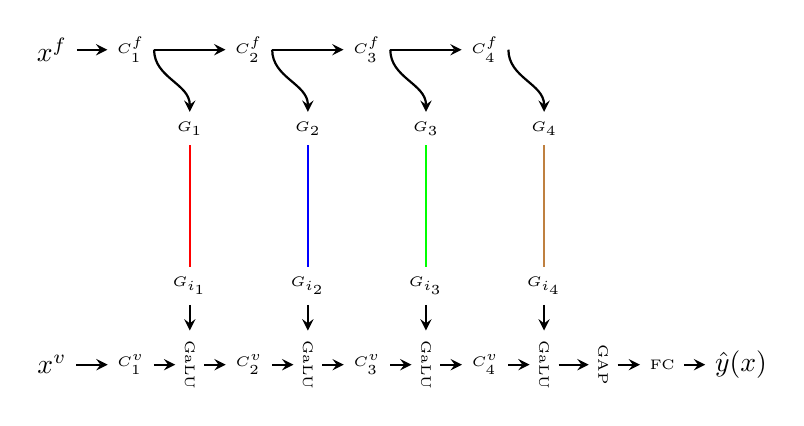
\begin{tikzpicture}
%\node []  (fntext)at (-4.625,-3.5) {CNN-GAP-DLGN};

%\node []  (output) at (7.5,1.5) {$\hat{y}(x)$};


\node [] (dgn1-f-c4) at (-3.5,1.5){\tiny{$C^{\text{f}}_4$}};
\node [] (dgn1-f-c3) at (-5,1.5){\tiny{$C^{\text{f}}_3$}};
\node [] (dgn1-f-c2) at (-6.5,1.5){\tiny{$C^{\text{f}}_2$}};
\node [] (dgn1-f-c1) at (-8,1.5){\tiny{$C^{\text{f}}_1$}};
\node [] (dgn1-input-f) at (-9,1.5){$x^{\text{f}}$};
\draw [-stealth,thick]   (dgn1-f-c3.east) -- (dgn1-f-c4.west);
\draw [-stealth,thick]   (dgn1-f-c2.east) -- (dgn1-f-c3.west);
\draw [-stealth,thick]   (dgn1-f-c1.east) -- (dgn1-f-c2.west);
\draw [-stealth,thick]   (dgn1-input-f.east) -- (dgn1-f-c1.west);



\node []  (dgn1-output) at (-0.25,-2.5) {$\hat{y}(x)$};

\node [] (dgn1-smax) at (-1.25,-2.5){\tiny{FC}};
\draw [-stealth,thick]   (dgn1-smax.east)--(dgn1-output.west);

\node [rotate=-90] (dgn1-gap) at (-2,-2.5){\tiny{GAP}};
\draw [-stealth,thick]   (dgn1-gap.north)--(dgn1-smax.west);


\node [rotate=-90] (dgn1-galu-4) at (-2.75,-2.5){\tiny{GaLU}};
\draw [-stealth,thick]   (dgn1-galu-4.north)--(dgn1-gap.south);

\node [] (dgn1-v-c4) at (-3.5,-2.5){\tiny{$C^{\text{v}}_4$}};
\draw [-stealth,thick]   (dgn1-v-c4.east) -- (dgn1-galu-4.south);


\node [rotate=-90] (dgn1-galu-3) at (-4.25,-2.5){\tiny{GaLU}};
\draw [-stealth,thick]   (dgn1-galu-3.north) -- (dgn1-v-c4.west);

\node [] (dgn1-v-c3) at (-5,-2.5){\tiny{$C^{\text{v}}_3$}};
\draw [-stealth,thick]   (dgn1-v-c3.east) -- (dgn1-galu-3.south);


\node [rotate=-90] (dgn1-galu-2) at (-5.75,-2.5){\tiny{GaLU}};
\draw [-stealth,thick]   (dgn1-galu-2.north) -- (dgn1-v-c3.west);

\node [] (dgn1-v-c2) at (-6.5,-2.5){\tiny{$C^{\text{v}}_2$}};
\draw [-stealth,thick]   (dgn1-v-c2.east) -- (dgn1-galu-2.south);


\node [rotate=-90] (dgn1-galu-1) at (-7.25,-2.5){\tiny{GaLU}};
\draw [-stealth,thick]   (dgn1-galu-1.north) -- (dgn1-v-c2.west);


\node [] (dgn1-v-c1) at (-8,-2.5){\tiny{$C^{\text{v}}_1$}};
\draw [-stealth,thick]   (dgn1-v-c1.east) -- (dgn1-galu-1.south);


\node [] (dgn1-v-input) at (-9,-2.5){$x^{\text{v}}$};

\draw [-stealth,thick]   (dgn1-v-input.east) -- (dgn1-v-c1.west);


\node[] (dgn1-gating-4-up) at (-2.75,0.5){\tiny{$G_{4}$}};
\draw [-stealth,thick]   (dgn1-f-c4.east) to[out=-90,in=90] (dgn1-gating-4-up.north);


\node[] (dgn1-gating-3-up) at (-4.25,0.5){\tiny{$G_{3}$}};
\draw [-stealth,thick]   (dgn1-f-c3.east) to[out=-90,in=90] (dgn1-gating-3-up.north);



\node[] (dgn1-gating-2-up) at (-5.75,0.5){\tiny{$G_{2}$}};
\draw [-stealth,thick]   (dgn1-f-c2.east) to[out=-90,in=90] (dgn1-gating-2-up.north);


\node[] (dgn1-gating-1-up) at (-7.25,0.5){\tiny{$G_{1}$}};
\draw [-stealth,thick]   (dgn1-f-c1.east) to[out=-90,in=90] (dgn1-gating-1-up.north);





\node[] (dgn1-gating-4) at (-2.75,-1.5){\tiny{$G_{i_4}$}};
\draw [-stealth,thick]   (dgn1-gating-4.south) -- (dgn1-galu-4.west);


\node[] (dgn1-gating-3) at (-4.25,-1.5){\tiny{$G_{i_3}$}};
\draw [-stealth,thick]   (dgn1-gating-3.south) -- (dgn1-galu-3.west);



\node[] (dgn1-gating-2) at (-5.75,-1.5){\tiny{$G_{i_2}$}};
\draw [-stealth,thick]   (dgn1-gating-2.south) -- (dgn1-galu-2.west);


\node[] (dgn1-gating-1) at (-7.25,-1.5){\tiny{$G_{i_1}$}};
\draw [-stealth,thick]   (dgn1-gating-1.south) -- (dgn1-galu-1.west);



\draw [-,thick,color=red]   (dgn1-gating-1-up.south) --(dgn1-gating-1.north);

\draw [-,thick,color=blue]   (dgn1-gating-2-up.south) --(dgn1-gating-2.north);

\draw [-,thick,color=green]   (dgn1-gating-3-up.south) --(dgn1-gating-3.north);

\draw [-,thick,color=brown]   (dgn1-gating-4-up.south) --(dgn1-gating-4.north);


%%%%%%%%%%%%%%%%%%%%%%%%%%%%%%%%%%%%%%%%%%%%%%%%%%%%%%%%%%%%%%%%%
	
\end{tikzpicture}


}
\end{minipage}
\begin{minipage}{0.48\columnwidth}
\centering
\resizebox{0.99\columnwidth}{!}{
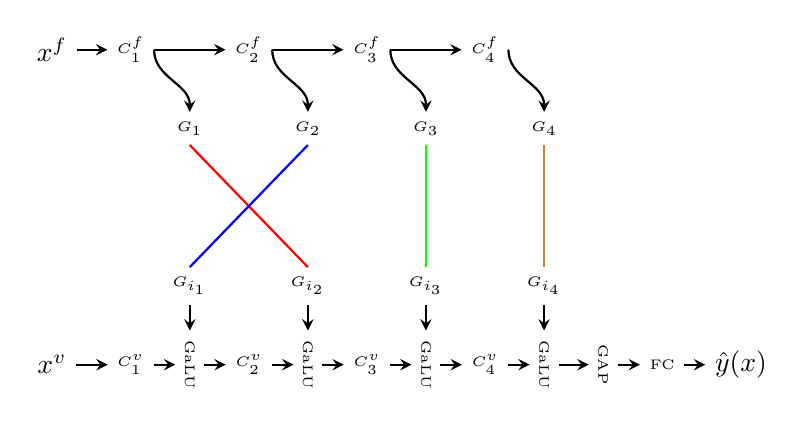
\begin{tikzpicture}
%\node []  (fntext)at (-4.625,-3.5) {CNN-GAP-DLGN};

%\node []  (output) at (7.5,1.5) {$\hat{y}(x)$};


\node [] (dgn1-f-c4) at (-3.5,1.5){\tiny{$C^{\text{f}}_4$}};
\node [] (dgn1-f-c3) at (-5,1.5){\tiny{$C^{\text{f}}_3$}};
\node [] (dgn1-f-c2) at (-6.5,1.5){\tiny{$C^{\text{f}}_2$}};
\node [] (dgn1-f-c1) at (-8,1.5){\tiny{$C^{\text{f}}_1$}};
\node [] (dgn1-input-f) at (-9,1.5){$x^{\text{f}}$};
\draw [-stealth,thick]   (dgn1-f-c3.east) -- (dgn1-f-c4.west);
\draw [-stealth,thick]   (dgn1-f-c2.east) -- (dgn1-f-c3.west);
\draw [-stealth,thick]   (dgn1-f-c1.east) -- (dgn1-f-c2.west);
\draw [-stealth,thick]   (dgn1-input-f.east) -- (dgn1-f-c1.west);



\node []  (dgn1-output) at (-0.25,-2.5) {$\hat{y}(x)$};

\node [] (dgn1-smax) at (-1.25,-2.5){\tiny{FC}};
\draw [-stealth,thick]   (dgn1-smax.east)--(dgn1-output.west);

\node [rotate=-90] (dgn1-gap) at (-2,-2.5){\tiny{GAP}};
\draw [-stealth,thick]   (dgn1-gap.north)--(dgn1-smax.west);


\node [rotate=-90] (dgn1-galu-4) at (-2.75,-2.5){\tiny{GaLU}};
\draw [-stealth,thick]   (dgn1-galu-4.north)--(dgn1-gap.south);

\node [] (dgn1-v-c4) at (-3.5,-2.5){\tiny{$C^{\text{v}}_4$}};
\draw [-stealth,thick]   (dgn1-v-c4.east) -- (dgn1-galu-4.south);


\node [rotate=-90] (dgn1-galu-3) at (-4.25,-2.5){\tiny{GaLU}};
\draw [-stealth,thick]   (dgn1-galu-3.north) -- (dgn1-v-c4.west);

\node [] (dgn1-v-c3) at (-5,-2.5){\tiny{$C^{\text{v}}_3$}};
\draw [-stealth,thick]   (dgn1-v-c3.east) -- (dgn1-galu-3.south);


\node [rotate=-90] (dgn1-galu-2) at (-5.75,-2.5){\tiny{GaLU}};
\draw [-stealth,thick]   (dgn1-galu-2.north) -- (dgn1-v-c3.west);

\node [] (dgn1-v-c2) at (-6.5,-2.5){\tiny{$C^{\text{v}}_2$}};
\draw [-stealth,thick]   (dgn1-v-c2.east) -- (dgn1-galu-2.south);


\node [rotate=-90] (dgn1-galu-1) at (-7.25,-2.5){\tiny{GaLU}};
\draw [-stealth,thick]   (dgn1-galu-1.north) -- (dgn1-v-c2.west);


\node [] (dgn1-v-c1) at (-8,-2.5){\tiny{$C^{\text{v}}_1$}};
\draw [-stealth,thick]   (dgn1-v-c1.east) -- (dgn1-galu-1.south);


\node [] (dgn1-v-input) at (-9,-2.5){$x^{\text{v}}$};

\draw [-stealth,thick]   (dgn1-v-input.east) -- (dgn1-v-c1.west);


\node[] (dgn1-gating-4-up) at (-2.75,0.5){\tiny{$G_{4}$}};
\draw [-stealth,thick]   (dgn1-f-c4.east) to[out=-90,in=90] (dgn1-gating-4-up.north);


\node[] (dgn1-gating-3-up) at (-4.25,0.5){\tiny{$G_{3}$}};
\draw [-stealth,thick]   (dgn1-f-c3.east) to[out=-90,in=90] (dgn1-gating-3-up.north);



\node[] (dgn1-gating-2-up) at (-5.75,0.5){\tiny{$G_{2}$}};
\draw [-stealth,thick]   (dgn1-f-c2.east) to[out=-90,in=90] (dgn1-gating-2-up.north);


\node[] (dgn1-gating-1-up) at (-7.25,0.5){\tiny{$G_{1}$}};
\draw [-stealth,thick]   (dgn1-f-c1.east) to[out=-90,in=90] (dgn1-gating-1-up.north);





\node[] (dgn1-gating-4) at (-2.75,-1.5){\tiny{$G_{i_4}$}};
\draw [-stealth,thick]   (dgn1-gating-4.south) -- (dgn1-galu-4.west);


\node[] (dgn1-gating-3) at (-4.25,-1.5){\tiny{$G_{i_3}$}};
\draw [-stealth,thick]   (dgn1-gating-3.south) -- (dgn1-galu-3.west);



\node[] (dgn1-gating-2) at (-5.75,-1.5){\tiny{$G_{i_2}$}};
\draw [-stealth,thick]   (dgn1-gating-2.south) -- (dgn1-galu-2.west);


\node[] (dgn1-gating-1) at (-7.25,-1.5){\tiny{$G_{i_1}$}};
\draw [-stealth,thick]   (dgn1-gating-1.south) -- (dgn1-galu-1.west);



\draw [-,thick,color=red]   (dgn1-gating-1-up.south) --(dgn1-gating-2.north);

\draw [-,thick,color=blue]   (dgn1-gating-2-up.south) --(dgn1-gating-1.north);

\draw [-,thick,color=green]   (dgn1-gating-3-up.south) --(dgn1-gating-3.north);

\draw [-,thick,color=brown]   (dgn1-gating-4-up.south) --(dgn1-gating-4.north);


%%%%%%%%%%%%%%%%%%%%%%%%%%%%%%%%%%%%%%%%%%%%%%%%%%%%%%%%%%%%%%%%%
	
\end{tikzpicture}


}
\end{minipage}

\begin{minipage}{0.48\columnwidth}
\centering
\resizebox{0.99\columnwidth}{!}{
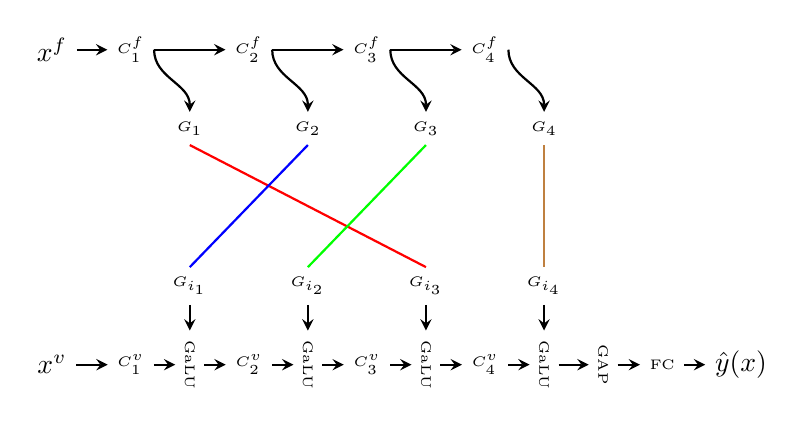
\begin{tikzpicture}
%\node []  (fntext)at (-4.625,-3.5) {CNN-GAP-DLGN};

%\node []  (output) at (7.5,1.5) {$\hat{y}(x)$};


\node [] (dgn1-f-c4) at (-3.5,1.5){\tiny{$C^{\text{f}}_4$}};
\node [] (dgn1-f-c3) at (-5,1.5){\tiny{$C^{\text{f}}_3$}};
\node [] (dgn1-f-c2) at (-6.5,1.5){\tiny{$C^{\text{f}}_2$}};
\node [] (dgn1-f-c1) at (-8,1.5){\tiny{$C^{\text{f}}_1$}};
\node [] (dgn1-input-f) at (-9,1.5){$x^{\text{f}}$};
\draw [-stealth,thick]   (dgn1-f-c3.east) -- (dgn1-f-c4.west);
\draw [-stealth,thick]   (dgn1-f-c2.east) -- (dgn1-f-c3.west);
\draw [-stealth,thick]   (dgn1-f-c1.east) -- (dgn1-f-c2.west);
\draw [-stealth,thick]   (dgn1-input-f.east) -- (dgn1-f-c1.west);



\node []  (dgn1-output) at (-0.25,-2.5) {$\hat{y}(x)$};

\node [] (dgn1-smax) at (-1.25,-2.5){\tiny{FC}};
\draw [-stealth,thick]   (dgn1-smax.east)--(dgn1-output.west);

\node [rotate=-90] (dgn1-gap) at (-2,-2.5){\tiny{GAP}};
\draw [-stealth,thick]   (dgn1-gap.north)--(dgn1-smax.west);


\node [rotate=-90] (dgn1-galu-4) at (-2.75,-2.5){\tiny{GaLU}};
\draw [-stealth,thick]   (dgn1-galu-4.north)--(dgn1-gap.south);

\node [] (dgn1-v-c4) at (-3.5,-2.5){\tiny{$C^{\text{v}}_4$}};
\draw [-stealth,thick]   (dgn1-v-c4.east) -- (dgn1-galu-4.south);


\node [rotate=-90] (dgn1-galu-3) at (-4.25,-2.5){\tiny{GaLU}};
\draw [-stealth,thick]   (dgn1-galu-3.north) -- (dgn1-v-c4.west);

\node [] (dgn1-v-c3) at (-5,-2.5){\tiny{$C^{\text{v}}_3$}};
\draw [-stealth,thick]   (dgn1-v-c3.east) -- (dgn1-galu-3.south);


\node [rotate=-90] (dgn1-galu-2) at (-5.75,-2.5){\tiny{GaLU}};
\draw [-stealth,thick]   (dgn1-galu-2.north) -- (dgn1-v-c3.west);

\node [] (dgn1-v-c2) at (-6.5,-2.5){\tiny{$C^{\text{v}}_2$}};
\draw [-stealth,thick]   (dgn1-v-c2.east) -- (dgn1-galu-2.south);


\node [rotate=-90] (dgn1-galu-1) at (-7.25,-2.5){\tiny{GaLU}};
\draw [-stealth,thick]   (dgn1-galu-1.north) -- (dgn1-v-c2.west);


\node [] (dgn1-v-c1) at (-8,-2.5){\tiny{$C^{\text{v}}_1$}};
\draw [-stealth,thick]   (dgn1-v-c1.east) -- (dgn1-galu-1.south);


\node [] (dgn1-v-input) at (-9,-2.5){$x^{\text{v}}$};

\draw [-stealth,thick]   (dgn1-v-input.east) -- (dgn1-v-c1.west);


\node[] (dgn1-gating-4-up) at (-2.75,0.5){\tiny{$G_{4}$}};
\draw [-stealth,thick]   (dgn1-f-c4.east) to[out=-90,in=90] (dgn1-gating-4-up.north);


\node[] (dgn1-gating-3-up) at (-4.25,0.5){\tiny{$G_{3}$}};
\draw [-stealth,thick]   (dgn1-f-c3.east) to[out=-90,in=90] (dgn1-gating-3-up.north);



\node[] (dgn1-gating-2-up) at (-5.75,0.5){\tiny{$G_{2}$}};
\draw [-stealth,thick]   (dgn1-f-c2.east) to[out=-90,in=90] (dgn1-gating-2-up.north);


\node[] (dgn1-gating-1-up) at (-7.25,0.5){\tiny{$G_{1}$}};
\draw [-stealth,thick]   (dgn1-f-c1.east) to[out=-90,in=90] (dgn1-gating-1-up.north);





\node[] (dgn1-gating-4) at (-2.75,-1.5){\tiny{$G_{i_4}$}};
\draw [-stealth,thick]   (dgn1-gating-4.south) -- (dgn1-galu-4.west);


\node[] (dgn1-gating-3) at (-4.25,-1.5){\tiny{$G_{i_3}$}};
\draw [-stealth,thick]   (dgn1-gating-3.south) -- (dgn1-galu-3.west);



\node[] (dgn1-gating-2) at (-5.75,-1.5){\tiny{$G_{i_2}$}};
\draw [-stealth,thick]   (dgn1-gating-2.south) -- (dgn1-galu-2.west);


\node[] (dgn1-gating-1) at (-7.25,-1.5){\tiny{$G_{i_1}$}};
\draw [-stealth,thick]   (dgn1-gating-1.south) -- (dgn1-galu-1.west);



\draw [-,thick,color=red]   (dgn1-gating-1-up.south) --(dgn1-gating-3.north);

\draw [-,thick,color=blue]   (dgn1-gating-2-up.south) --(dgn1-gating-1.north);

\draw [-,thick,color=green]   (dgn1-gating-3-up.south) --(dgn1-gating-2.north);

\draw [-,thick,color=brown]   (dgn1-gating-4-up.south) --(dgn1-gating-4.north);


%%%%%%%%%%%%%%%%%%%%%%%%%%%%%%%%%%%%%%%%%%%%%%%%%%%%%%%%%%%%%%%%%
	
\end{tikzpicture}


}
\end{minipage}
\begin{minipage}{0.48\columnwidth}
\centering
\resizebox{0.99\columnwidth}{!}{
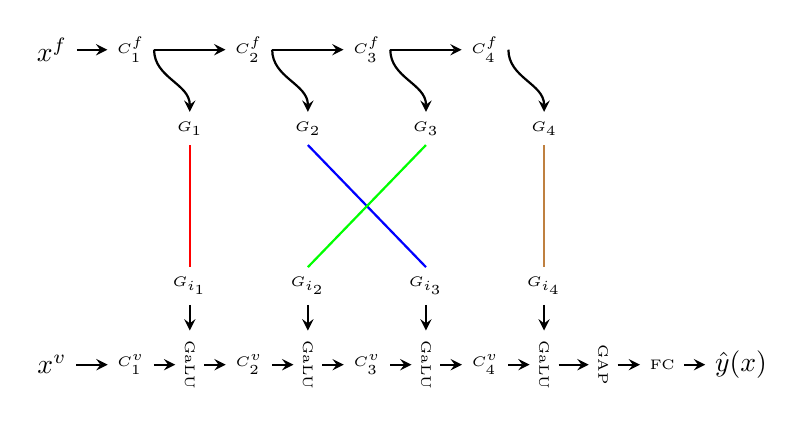
\begin{tikzpicture}
%\node []  (fntext)at (-4.625,-3.5) {CNN-GAP-DLGN};

%\node []  (output) at (7.5,1.5) {$\hat{y}(x)$};


\node [] (dgn1-f-c4) at (-3.5,1.5){\tiny{$C^{\text{f}}_4$}};
\node [] (dgn1-f-c3) at (-5,1.5){\tiny{$C^{\text{f}}_3$}};
\node [] (dgn1-f-c2) at (-6.5,1.5){\tiny{$C^{\text{f}}_2$}};
\node [] (dgn1-f-c1) at (-8,1.5){\tiny{$C^{\text{f}}_1$}};
\node [] (dgn1-input-f) at (-9,1.5){$x^{\text{f}}$};
\draw [-stealth,thick]   (dgn1-f-c3.east) -- (dgn1-f-c4.west);
\draw [-stealth,thick]   (dgn1-f-c2.east) -- (dgn1-f-c3.west);
\draw [-stealth,thick]   (dgn1-f-c1.east) -- (dgn1-f-c2.west);
\draw [-stealth,thick]   (dgn1-input-f.east) -- (dgn1-f-c1.west);



\node []  (dgn1-output) at (-0.25,-2.5) {$\hat{y}(x)$};

\node [] (dgn1-smax) at (-1.25,-2.5){\tiny{FC}};
\draw [-stealth,thick]   (dgn1-smax.east)--(dgn1-output.west);

\node [rotate=-90] (dgn1-gap) at (-2,-2.5){\tiny{GAP}};
\draw [-stealth,thick]   (dgn1-gap.north)--(dgn1-smax.west);


\node [rotate=-90] (dgn1-galu-4) at (-2.75,-2.5){\tiny{GaLU}};
\draw [-stealth,thick]   (dgn1-galu-4.north)--(dgn1-gap.south);

\node [] (dgn1-v-c4) at (-3.5,-2.5){\tiny{$C^{\text{v}}_4$}};
\draw [-stealth,thick]   (dgn1-v-c4.east) -- (dgn1-galu-4.south);


\node [rotate=-90] (dgn1-galu-3) at (-4.25,-2.5){\tiny{GaLU}};
\draw [-stealth,thick]   (dgn1-galu-3.north) -- (dgn1-v-c4.west);

\node [] (dgn1-v-c3) at (-5,-2.5){\tiny{$C^{\text{v}}_3$}};
\draw [-stealth,thick]   (dgn1-v-c3.east) -- (dgn1-galu-3.south);


\node [rotate=-90] (dgn1-galu-2) at (-5.75,-2.5){\tiny{GaLU}};
\draw [-stealth,thick]   (dgn1-galu-2.north) -- (dgn1-v-c3.west);

\node [] (dgn1-v-c2) at (-6.5,-2.5){\tiny{$C^{\text{v}}_2$}};
\draw [-stealth,thick]   (dgn1-v-c2.east) -- (dgn1-galu-2.south);


\node [rotate=-90] (dgn1-galu-1) at (-7.25,-2.5){\tiny{GaLU}};
\draw [-stealth,thick]   (dgn1-galu-1.north) -- (dgn1-v-c2.west);


\node [] (dgn1-v-c1) at (-8,-2.5){\tiny{$C^{\text{v}}_1$}};
\draw [-stealth,thick]   (dgn1-v-c1.east) -- (dgn1-galu-1.south);


\node [] (dgn1-v-input) at (-9,-2.5){$x^{\text{v}}$};

\draw [-stealth,thick]   (dgn1-v-input.east) -- (dgn1-v-c1.west);


\node[] (dgn1-gating-4-up) at (-2.75,0.5){\tiny{$G_{4}$}};
\draw [-stealth,thick]   (dgn1-f-c4.east) to[out=-90,in=90] (dgn1-gating-4-up.north);


\node[] (dgn1-gating-3-up) at (-4.25,0.5){\tiny{$G_{3}$}};
\draw [-stealth,thick]   (dgn1-f-c3.east) to[out=-90,in=90] (dgn1-gating-3-up.north);



\node[] (dgn1-gating-2-up) at (-5.75,0.5){\tiny{$G_{2}$}};
\draw [-stealth,thick]   (dgn1-f-c2.east) to[out=-90,in=90] (dgn1-gating-2-up.north);


\node[] (dgn1-gating-1-up) at (-7.25,0.5){\tiny{$G_{1}$}};
\draw [-stealth,thick]   (dgn1-f-c1.east) to[out=-90,in=90] (dgn1-gating-1-up.north);





\node[] (dgn1-gating-4) at (-2.75,-1.5){\tiny{$G_{i_4}$}};
\draw [-stealth,thick]   (dgn1-gating-4.south) -- (dgn1-galu-4.west);


\node[] (dgn1-gating-3) at (-4.25,-1.5){\tiny{$G_{i_3}$}};
\draw [-stealth,thick]   (dgn1-gating-3.south) -- (dgn1-galu-3.west);



\node[] (dgn1-gating-2) at (-5.75,-1.5){\tiny{$G_{i_2}$}};
\draw [-stealth,thick]   (dgn1-gating-2.south) -- (dgn1-galu-2.west);


\node[] (dgn1-gating-1) at (-7.25,-1.5){\tiny{$G_{i_1}$}};
\draw [-stealth,thick]   (dgn1-gating-1.south) -- (dgn1-galu-1.west);



\draw [-,thick,color=red]   (dgn1-gating-1-up.south) --(dgn1-gating-1.north);

\draw [-,thick,color=blue]   (dgn1-gating-2-up.south) --(dgn1-gating-3.north);

\draw [-,thick,color=green]   (dgn1-gating-3-up.south) --(dgn1-gating-2.north);

\draw [-,thick,color=brown]   (dgn1-gating-4-up.south) --(dgn1-gating-4.north);


%%%%%%%%%%%%%%%%%%%%%%%%%%%%%%%%%%%%%%%%%%%%%%%%%%%%%%%%%%%%%%%%%
	
\end{tikzpicture}


}
\end{minipage}


\begin{minipage}{0.48\columnwidth}
\centering
\resizebox{0.99\columnwidth}{!}{
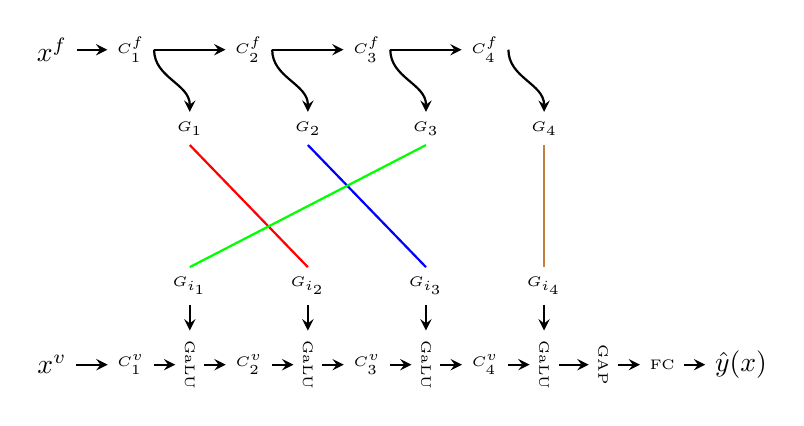
\begin{tikzpicture}
%\node []  (fntext)at (-4.625,-3.5) {CNN-GAP-DLGN};

%\node []  (output) at (7.5,1.5) {$\hat{y}(x)$};


\node [] (dgn1-f-c4) at (-3.5,1.5){\tiny{$C^{\text{f}}_4$}};
\node [] (dgn1-f-c3) at (-5,1.5){\tiny{$C^{\text{f}}_3$}};
\node [] (dgn1-f-c2) at (-6.5,1.5){\tiny{$C^{\text{f}}_2$}};
\node [] (dgn1-f-c1) at (-8,1.5){\tiny{$C^{\text{f}}_1$}};
\node [] (dgn1-input-f) at (-9,1.5){$x^{\text{f}}$};
\draw [-stealth,thick]   (dgn1-f-c3.east) -- (dgn1-f-c4.west);
\draw [-stealth,thick]   (dgn1-f-c2.east) -- (dgn1-f-c3.west);
\draw [-stealth,thick]   (dgn1-f-c1.east) -- (dgn1-f-c2.west);
\draw [-stealth,thick]   (dgn1-input-f.east) -- (dgn1-f-c1.west);



\node []  (dgn1-output) at (-0.25,-2.5) {$\hat{y}(x)$};

\node [] (dgn1-smax) at (-1.25,-2.5){\tiny{FC}};
\draw [-stealth,thick]   (dgn1-smax.east)--(dgn1-output.west);

\node [rotate=-90] (dgn1-gap) at (-2,-2.5){\tiny{GAP}};
\draw [-stealth,thick]   (dgn1-gap.north)--(dgn1-smax.west);


\node [rotate=-90] (dgn1-galu-4) at (-2.75,-2.5){\tiny{GaLU}};
\draw [-stealth,thick]   (dgn1-galu-4.north)--(dgn1-gap.south);

\node [] (dgn1-v-c4) at (-3.5,-2.5){\tiny{$C^{\text{v}}_4$}};
\draw [-stealth,thick]   (dgn1-v-c4.east) -- (dgn1-galu-4.south);


\node [rotate=-90] (dgn1-galu-3) at (-4.25,-2.5){\tiny{GaLU}};
\draw [-stealth,thick]   (dgn1-galu-3.north) -- (dgn1-v-c4.west);

\node [] (dgn1-v-c3) at (-5,-2.5){\tiny{$C^{\text{v}}_3$}};
\draw [-stealth,thick]   (dgn1-v-c3.east) -- (dgn1-galu-3.south);


\node [rotate=-90] (dgn1-galu-2) at (-5.75,-2.5){\tiny{GaLU}};
\draw [-stealth,thick]   (dgn1-galu-2.north) -- (dgn1-v-c3.west);

\node [] (dgn1-v-c2) at (-6.5,-2.5){\tiny{$C^{\text{v}}_2$}};
\draw [-stealth,thick]   (dgn1-v-c2.east) -- (dgn1-galu-2.south);


\node [rotate=-90] (dgn1-galu-1) at (-7.25,-2.5){\tiny{GaLU}};
\draw [-stealth,thick]   (dgn1-galu-1.north) -- (dgn1-v-c2.west);


\node [] (dgn1-v-c1) at (-8,-2.5){\tiny{$C^{\text{v}}_1$}};
\draw [-stealth,thick]   (dgn1-v-c1.east) -- (dgn1-galu-1.south);


\node [] (dgn1-v-input) at (-9,-2.5){$x^{\text{v}}$};

\draw [-stealth,thick]   (dgn1-v-input.east) -- (dgn1-v-c1.west);


\node[] (dgn1-gating-4-up) at (-2.75,0.5){\tiny{$G_{4}$}};
\draw [-stealth,thick]   (dgn1-f-c4.east) to[out=-90,in=90] (dgn1-gating-4-up.north);


\node[] (dgn1-gating-3-up) at (-4.25,0.5){\tiny{$G_{3}$}};
\draw [-stealth,thick]   (dgn1-f-c3.east) to[out=-90,in=90] (dgn1-gating-3-up.north);



\node[] (dgn1-gating-2-up) at (-5.75,0.5){\tiny{$G_{2}$}};
\draw [-stealth,thick]   (dgn1-f-c2.east) to[out=-90,in=90] (dgn1-gating-2-up.north);


\node[] (dgn1-gating-1-up) at (-7.25,0.5){\tiny{$G_{1}$}};
\draw [-stealth,thick]   (dgn1-f-c1.east) to[out=-90,in=90] (dgn1-gating-1-up.north);





\node[] (dgn1-gating-4) at (-2.75,-1.5){\tiny{$G_{i_4}$}};
\draw [-stealth,thick]   (dgn1-gating-4.south) -- (dgn1-galu-4.west);


\node[] (dgn1-gating-3) at (-4.25,-1.5){\tiny{$G_{i_3}$}};
\draw [-stealth,thick]   (dgn1-gating-3.south) -- (dgn1-galu-3.west);



\node[] (dgn1-gating-2) at (-5.75,-1.5){\tiny{$G_{i_2}$}};
\draw [-stealth,thick]   (dgn1-gating-2.south) -- (dgn1-galu-2.west);


\node[] (dgn1-gating-1) at (-7.25,-1.5){\tiny{$G_{i_1}$}};
\draw [-stealth,thick]   (dgn1-gating-1.south) -- (dgn1-galu-1.west);



\draw [-,thick,color=red]   (dgn1-gating-1-up.south) --(dgn1-gating-2.north);

\draw [-,thick,color=blue]   (dgn1-gating-2-up.south) --(dgn1-gating-3.north);

\draw [-,thick,color=green]   (dgn1-gating-3-up.south) --(dgn1-gating-1.north);

\draw [-,thick,color=brown]   (dgn1-gating-4-up.south) --(dgn1-gating-4.north);


%%%%%%%%%%%%%%%%%%%%%%%%%%%%%%%%%%%%%%%%%%%%%%%%%%%%%%%%%%%%%%%%%
	
\end{tikzpicture}


}
\end{minipage}
\begin{minipage}{0.48\columnwidth}
\centering
\resizebox{0.99\columnwidth}{!}{
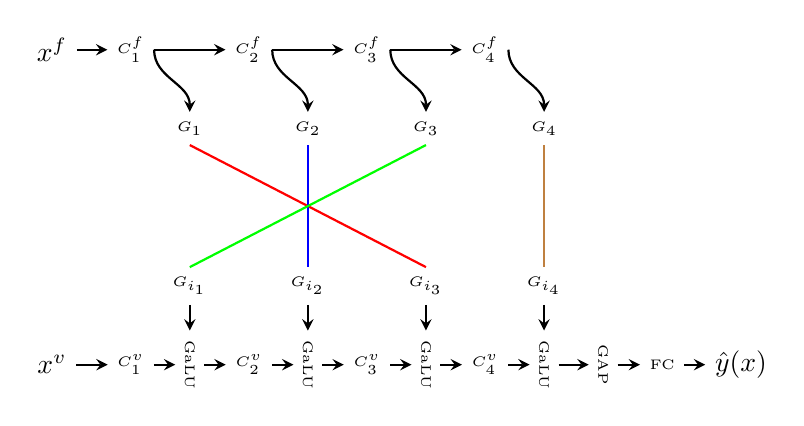
\begin{tikzpicture}
%\node []  (fntext)at (-4.625,-3.5) {CNN-GAP-DLGN};

%\node []  (output) at (7.5,1.5) {$\hat{y}(x)$};


\node [] (dgn1-f-c4) at (-3.5,1.5){\tiny{$C^{\text{f}}_4$}};
\node [] (dgn1-f-c3) at (-5,1.5){\tiny{$C^{\text{f}}_3$}};
\node [] (dgn1-f-c2) at (-6.5,1.5){\tiny{$C^{\text{f}}_2$}};
\node [] (dgn1-f-c1) at (-8,1.5){\tiny{$C^{\text{f}}_1$}};
\node [] (dgn1-input-f) at (-9,1.5){$x^{\text{f}}$};
\draw [-stealth,thick]   (dgn1-f-c3.east) -- (dgn1-f-c4.west);
\draw [-stealth,thick]   (dgn1-f-c2.east) -- (dgn1-f-c3.west);
\draw [-stealth,thick]   (dgn1-f-c1.east) -- (dgn1-f-c2.west);
\draw [-stealth,thick]   (dgn1-input-f.east) -- (dgn1-f-c1.west);



\node []  (dgn1-output) at (-0.25,-2.5) {$\hat{y}(x)$};

\node [] (dgn1-smax) at (-1.25,-2.5){\tiny{FC}};
\draw [-stealth,thick]   (dgn1-smax.east)--(dgn1-output.west);

\node [rotate=-90] (dgn1-gap) at (-2,-2.5){\tiny{GAP}};
\draw [-stealth,thick]   (dgn1-gap.north)--(dgn1-smax.west);


\node [rotate=-90] (dgn1-galu-4) at (-2.75,-2.5){\tiny{GaLU}};
\draw [-stealth,thick]   (dgn1-galu-4.north)--(dgn1-gap.south);

\node [] (dgn1-v-c4) at (-3.5,-2.5){\tiny{$C^{\text{v}}_4$}};
\draw [-stealth,thick]   (dgn1-v-c4.east) -- (dgn1-galu-4.south);


\node [rotate=-90] (dgn1-galu-3) at (-4.25,-2.5){\tiny{GaLU}};
\draw [-stealth,thick]   (dgn1-galu-3.north) -- (dgn1-v-c4.west);

\node [] (dgn1-v-c3) at (-5,-2.5){\tiny{$C^{\text{v}}_3$}};
\draw [-stealth,thick]   (dgn1-v-c3.east) -- (dgn1-galu-3.south);


\node [rotate=-90] (dgn1-galu-2) at (-5.75,-2.5){\tiny{GaLU}};
\draw [-stealth,thick]   (dgn1-galu-2.north) -- (dgn1-v-c3.west);

\node [] (dgn1-v-c2) at (-6.5,-2.5){\tiny{$C^{\text{v}}_2$}};
\draw [-stealth,thick]   (dgn1-v-c2.east) -- (dgn1-galu-2.south);


\node [rotate=-90] (dgn1-galu-1) at (-7.25,-2.5){\tiny{GaLU}};
\draw [-stealth,thick]   (dgn1-galu-1.north) -- (dgn1-v-c2.west);


\node [] (dgn1-v-c1) at (-8,-2.5){\tiny{$C^{\text{v}}_1$}};
\draw [-stealth,thick]   (dgn1-v-c1.east) -- (dgn1-galu-1.south);


\node [] (dgn1-v-input) at (-9,-2.5){$x^{\text{v}}$};

\draw [-stealth,thick]   (dgn1-v-input.east) -- (dgn1-v-c1.west);


\node[] (dgn1-gating-4-up) at (-2.75,0.5){\tiny{$G_{4}$}};
\draw [-stealth,thick]   (dgn1-f-c4.east) to[out=-90,in=90] (dgn1-gating-4-up.north);


\node[] (dgn1-gating-3-up) at (-4.25,0.5){\tiny{$G_{3}$}};
\draw [-stealth,thick]   (dgn1-f-c3.east) to[out=-90,in=90] (dgn1-gating-3-up.north);



\node[] (dgn1-gating-2-up) at (-5.75,0.5){\tiny{$G_{2}$}};
\draw [-stealth,thick]   (dgn1-f-c2.east) to[out=-90,in=90] (dgn1-gating-2-up.north);


\node[] (dgn1-gating-1-up) at (-7.25,0.5){\tiny{$G_{1}$}};
\draw [-stealth,thick]   (dgn1-f-c1.east) to[out=-90,in=90] (dgn1-gating-1-up.north);





\node[] (dgn1-gating-4) at (-2.75,-1.5){\tiny{$G_{i_4}$}};
\draw [-stealth,thick]   (dgn1-gating-4.south) -- (dgn1-galu-4.west);


\node[] (dgn1-gating-3) at (-4.25,-1.5){\tiny{$G_{i_3}$}};
\draw [-stealth,thick]   (dgn1-gating-3.south) -- (dgn1-galu-3.west);



\node[] (dgn1-gating-2) at (-5.75,-1.5){\tiny{$G_{i_2}$}};
\draw [-stealth,thick]   (dgn1-gating-2.south) -- (dgn1-galu-2.west);


\node[] (dgn1-gating-1) at (-7.25,-1.5){\tiny{$G_{i_1}$}};
\draw [-stealth,thick]   (dgn1-gating-1.south) -- (dgn1-galu-1.west);



\draw [-,thick,color=red]   (dgn1-gating-1-up.south) --(dgn1-gating-3.north);

\draw [-,thick,color=blue]   (dgn1-gating-2-up.south) --(dgn1-gating-2.north);

\draw [-,thick,color=green]   (dgn1-gating-3-up.south) --(dgn1-gating-1.north);

\draw [-,thick,color=brown]   (dgn1-gating-4-up.south) --(dgn1-gating-4.north);


%%%%%%%%%%%%%%%%%%%%%%%%%%%%%%%%%%%%%%%%%%%%%%%%%%%%%%%%%%%%%%%%%
	
\end{tikzpicture}


}
\end{minipage}



\begin{minipage}{0.48\columnwidth}
\centering
\resizebox{0.99\columnwidth}{!}{
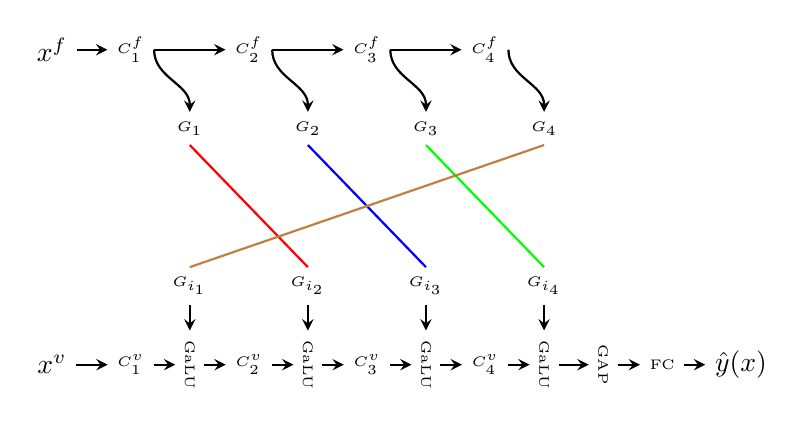
\begin{tikzpicture}
%\node []  (fntext)at (-4.625,-3.5) {CNN-GAP-DLGN};

%\node []  (output) at (7.5,1.5) {$\hat{y}(x)$};


\node [] (dgn1-f-c4) at (-3.5,1.5){\tiny{$C^{\text{f}}_4$}};
\node [] (dgn1-f-c3) at (-5,1.5){\tiny{$C^{\text{f}}_3$}};
\node [] (dgn1-f-c2) at (-6.5,1.5){\tiny{$C^{\text{f}}_2$}};
\node [] (dgn1-f-c1) at (-8,1.5){\tiny{$C^{\text{f}}_1$}};
\node [] (dgn1-input-f) at (-9,1.5){$x^{\text{f}}$};
\draw [-stealth,thick]   (dgn1-f-c3.east) -- (dgn1-f-c4.west);
\draw [-stealth,thick]   (dgn1-f-c2.east) -- (dgn1-f-c3.west);
\draw [-stealth,thick]   (dgn1-f-c1.east) -- (dgn1-f-c2.west);
\draw [-stealth,thick]   (dgn1-input-f.east) -- (dgn1-f-c1.west);



\node []  (dgn1-output) at (-0.25,-2.5) {$\hat{y}(x)$};

\node [] (dgn1-smax) at (-1.25,-2.5){\tiny{FC}};
\draw [-stealth,thick]   (dgn1-smax.east)--(dgn1-output.west);

\node [rotate=-90] (dgn1-gap) at (-2,-2.5){\tiny{GAP}};
\draw [-stealth,thick]   (dgn1-gap.north)--(dgn1-smax.west);


\node [rotate=-90] (dgn1-galu-4) at (-2.75,-2.5){\tiny{GaLU}};
\draw [-stealth,thick]   (dgn1-galu-4.north)--(dgn1-gap.south);

\node [] (dgn1-v-c4) at (-3.5,-2.5){\tiny{$C^{\text{v}}_4$}};
\draw [-stealth,thick]   (dgn1-v-c4.east) -- (dgn1-galu-4.south);


\node [rotate=-90] (dgn1-galu-3) at (-4.25,-2.5){\tiny{GaLU}};
\draw [-stealth,thick]   (dgn1-galu-3.north) -- (dgn1-v-c4.west);

\node [] (dgn1-v-c3) at (-5,-2.5){\tiny{$C^{\text{v}}_3$}};
\draw [-stealth,thick]   (dgn1-v-c3.east) -- (dgn1-galu-3.south);


\node [rotate=-90] (dgn1-galu-2) at (-5.75,-2.5){\tiny{GaLU}};
\draw [-stealth,thick]   (dgn1-galu-2.north) -- (dgn1-v-c3.west);

\node [] (dgn1-v-c2) at (-6.5,-2.5){\tiny{$C^{\text{v}}_2$}};
\draw [-stealth,thick]   (dgn1-v-c2.east) -- (dgn1-galu-2.south);


\node [rotate=-90] (dgn1-galu-1) at (-7.25,-2.5){\tiny{GaLU}};
\draw [-stealth,thick]   (dgn1-galu-1.north) -- (dgn1-v-c2.west);


\node [] (dgn1-v-c1) at (-8,-2.5){\tiny{$C^{\text{v}}_1$}};
\draw [-stealth,thick]   (dgn1-v-c1.east) -- (dgn1-galu-1.south);


\node [] (dgn1-v-input) at (-9,-2.5){$x^{\text{v}}$};

\draw [-stealth,thick]   (dgn1-v-input.east) -- (dgn1-v-c1.west);


\node[] (dgn1-gating-4-up) at (-2.75,0.5){\tiny{$G_{4}$}};
\draw [-stealth,thick]   (dgn1-f-c4.east) to[out=-90,in=90] (dgn1-gating-4-up.north);


\node[] (dgn1-gating-3-up) at (-4.25,0.5){\tiny{$G_{3}$}};
\draw [-stealth,thick]   (dgn1-f-c3.east) to[out=-90,in=90] (dgn1-gating-3-up.north);



\node[] (dgn1-gating-2-up) at (-5.75,0.5){\tiny{$G_{2}$}};
\draw [-stealth,thick]   (dgn1-f-c2.east) to[out=-90,in=90] (dgn1-gating-2-up.north);


\node[] (dgn1-gating-1-up) at (-7.25,0.5){\tiny{$G_{1}$}};
\draw [-stealth,thick]   (dgn1-f-c1.east) to[out=-90,in=90] (dgn1-gating-1-up.north);





\node[] (dgn1-gating-4) at (-2.75,-1.5){\tiny{$G_{i_4}$}};
\draw [-stealth,thick]   (dgn1-gating-4.south) -- (dgn1-galu-4.west);


\node[] (dgn1-gating-3) at (-4.25,-1.5){\tiny{$G_{i_3}$}};
\draw [-stealth,thick]   (dgn1-gating-3.south) -- (dgn1-galu-3.west);



\node[] (dgn1-gating-2) at (-5.75,-1.5){\tiny{$G_{i_2}$}};
\draw [-stealth,thick]   (dgn1-gating-2.south) -- (dgn1-galu-2.west);


\node[] (dgn1-gating-1) at (-7.25,-1.5){\tiny{$G_{i_1}$}};
\draw [-stealth,thick]   (dgn1-gating-1.south) -- (dgn1-galu-1.west);



\draw [-,thick,color=red]   (dgn1-gating-1-up.south) --(dgn1-gating-2.north);

\draw [-,thick,color=blue]   (dgn1-gating-2-up.south) --(dgn1-gating-3.north);

\draw [-,thick,color=green]   (dgn1-gating-3-up.south) --(dgn1-gating-4.north);

\draw [-,thick,color=brown]   (dgn1-gating-4-up.south) --(dgn1-gating-1.north);


%%%%%%%%%%%%%%%%%%%%%%%%%%%%%%%%%%%%%%%%%%%%%%%%%%%%%%%%%%%%%%%%%
	
\end{tikzpicture}


}
\end{minipage}
\begin{minipage}{0.48\columnwidth}
\centering
\resizebox{0.99\columnwidth}{!}{
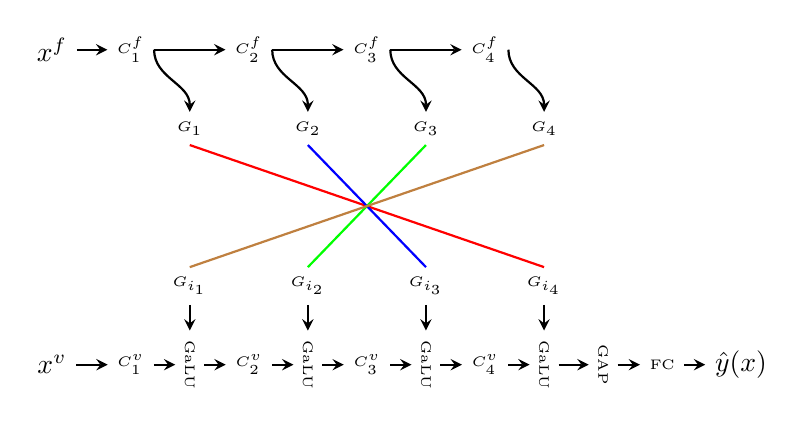
\begin{tikzpicture}
%\node []  (fntext)at (-4.625,-3.5) {CNN-GAP-DLGN};

%\node []  (output) at (7.5,1.5) {$\hat{y}(x)$};


\node [] (dgn1-f-c4) at (-3.5,1.5){\tiny{$C^{\text{f}}_4$}};
\node [] (dgn1-f-c3) at (-5,1.5){\tiny{$C^{\text{f}}_3$}};
\node [] (dgn1-f-c2) at (-6.5,1.5){\tiny{$C^{\text{f}}_2$}};
\node [] (dgn1-f-c1) at (-8,1.5){\tiny{$C^{\text{f}}_1$}};
\node [] (dgn1-input-f) at (-9,1.5){$x^{\text{f}}$};
\draw [-stealth,thick]   (dgn1-f-c3.east) -- (dgn1-f-c4.west);
\draw [-stealth,thick]   (dgn1-f-c2.east) -- (dgn1-f-c3.west);
\draw [-stealth,thick]   (dgn1-f-c1.east) -- (dgn1-f-c2.west);
\draw [-stealth,thick]   (dgn1-input-f.east) -- (dgn1-f-c1.west);



\node []  (dgn1-output) at (-0.25,-2.5) {$\hat{y}(x)$};

\node [] (dgn1-smax) at (-1.25,-2.5){\tiny{FC}};
\draw [-stealth,thick]   (dgn1-smax.east)--(dgn1-output.west);

\node [rotate=-90] (dgn1-gap) at (-2,-2.5){\tiny{GAP}};
\draw [-stealth,thick]   (dgn1-gap.north)--(dgn1-smax.west);


\node [rotate=-90] (dgn1-galu-4) at (-2.75,-2.5){\tiny{GaLU}};
\draw [-stealth,thick]   (dgn1-galu-4.north)--(dgn1-gap.south);

\node [] (dgn1-v-c4) at (-3.5,-2.5){\tiny{$C^{\text{v}}_4$}};
\draw [-stealth,thick]   (dgn1-v-c4.east) -- (dgn1-galu-4.south);


\node [rotate=-90] (dgn1-galu-3) at (-4.25,-2.5){\tiny{GaLU}};
\draw [-stealth,thick]   (dgn1-galu-3.north) -- (dgn1-v-c4.west);

\node [] (dgn1-v-c3) at (-5,-2.5){\tiny{$C^{\text{v}}_3$}};
\draw [-stealth,thick]   (dgn1-v-c3.east) -- (dgn1-galu-3.south);


\node [rotate=-90] (dgn1-galu-2) at (-5.75,-2.5){\tiny{GaLU}};
\draw [-stealth,thick]   (dgn1-galu-2.north) -- (dgn1-v-c3.west);

\node [] (dgn1-v-c2) at (-6.5,-2.5){\tiny{$C^{\text{v}}_2$}};
\draw [-stealth,thick]   (dgn1-v-c2.east) -- (dgn1-galu-2.south);


\node [rotate=-90] (dgn1-galu-1) at (-7.25,-2.5){\tiny{GaLU}};
\draw [-stealth,thick]   (dgn1-galu-1.north) -- (dgn1-v-c2.west);


\node [] (dgn1-v-c1) at (-8,-2.5){\tiny{$C^{\text{v}}_1$}};
\draw [-stealth,thick]   (dgn1-v-c1.east) -- (dgn1-galu-1.south);


\node [] (dgn1-v-input) at (-9,-2.5){$x^{\text{v}}$};

\draw [-stealth,thick]   (dgn1-v-input.east) -- (dgn1-v-c1.west);


\node[] (dgn1-gating-4-up) at (-2.75,0.5){\tiny{$G_{4}$}};
\draw [-stealth,thick]   (dgn1-f-c4.east) to[out=-90,in=90] (dgn1-gating-4-up.north);


\node[] (dgn1-gating-3-up) at (-4.25,0.5){\tiny{$G_{3}$}};
\draw [-stealth,thick]   (dgn1-f-c3.east) to[out=-90,in=90] (dgn1-gating-3-up.north);



\node[] (dgn1-gating-2-up) at (-5.75,0.5){\tiny{$G_{2}$}};
\draw [-stealth,thick]   (dgn1-f-c2.east) to[out=-90,in=90] (dgn1-gating-2-up.north);


\node[] (dgn1-gating-1-up) at (-7.25,0.5){\tiny{$G_{1}$}};
\draw [-stealth,thick]   (dgn1-f-c1.east) to[out=-90,in=90] (dgn1-gating-1-up.north);





\node[] (dgn1-gating-4) at (-2.75,-1.5){\tiny{$G_{i_4}$}};
\draw [-stealth,thick]   (dgn1-gating-4.south) -- (dgn1-galu-4.west);


\node[] (dgn1-gating-3) at (-4.25,-1.5){\tiny{$G_{i_3}$}};
\draw [-stealth,thick]   (dgn1-gating-3.south) -- (dgn1-galu-3.west);



\node[] (dgn1-gating-2) at (-5.75,-1.5){\tiny{$G_{i_2}$}};
\draw [-stealth,thick]   (dgn1-gating-2.south) -- (dgn1-galu-2.west);


\node[] (dgn1-gating-1) at (-7.25,-1.5){\tiny{$G_{i_1}$}};
\draw [-stealth,thick]   (dgn1-gating-1.south) -- (dgn1-galu-1.west);



\draw [-,thick,color=red]   (dgn1-gating-1-up.south) --(dgn1-gating-4.north);

\draw [-,thick,color=blue]   (dgn1-gating-2-up.south) --(dgn1-gating-3.north);

\draw [-,thick,color=green]   (dgn1-gating-3-up.south) --(dgn1-gating-2.north);

\draw [-,thick,color=brown]   (dgn1-gating-4-up.south) --(dgn1-gating-1.north);


%%%%%%%%%%%%%%%%%%%%%%%%%%%%%%%%%%%%%%%%%%%%%%%%%%%%%%%%%%%%%%%%%
	
\end{tikzpicture}


}
\end{minipage}

\begin{minipage}{0.48\columnwidth}
\centering
\resizebox{0.99\columnwidth}{!}{
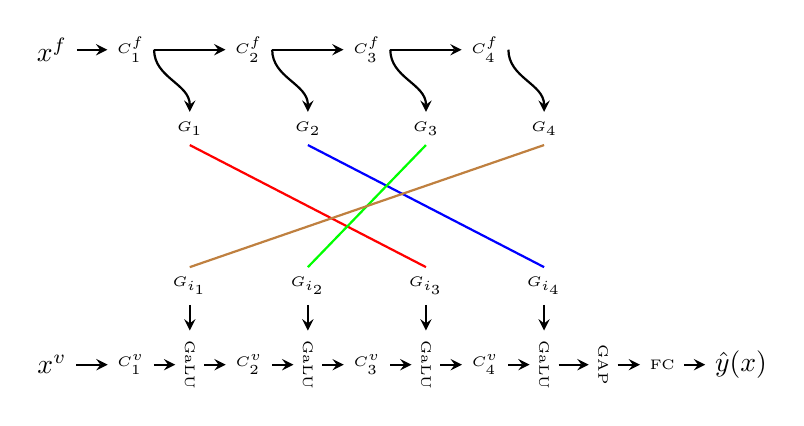
\begin{tikzpicture}
%\node []  (fntext)at (-4.625,-3.5) {CNN-GAP-DLGN};

%\node []  (output) at (7.5,1.5) {$\hat{y}(x)$};


\node [] (dgn1-f-c4) at (-3.5,1.5){\tiny{$C^{\text{f}}_4$}};
\node [] (dgn1-f-c3) at (-5,1.5){\tiny{$C^{\text{f}}_3$}};
\node [] (dgn1-f-c2) at (-6.5,1.5){\tiny{$C^{\text{f}}_2$}};
\node [] (dgn1-f-c1) at (-8,1.5){\tiny{$C^{\text{f}}_1$}};
\node [] (dgn1-input-f) at (-9,1.5){$x^{\text{f}}$};
\draw [-stealth,thick]   (dgn1-f-c3.east) -- (dgn1-f-c4.west);
\draw [-stealth,thick]   (dgn1-f-c2.east) -- (dgn1-f-c3.west);
\draw [-stealth,thick]   (dgn1-f-c1.east) -- (dgn1-f-c2.west);
\draw [-stealth,thick]   (dgn1-input-f.east) -- (dgn1-f-c1.west);



\node []  (dgn1-output) at (-0.25,-2.5) {$\hat{y}(x)$};

\node [] (dgn1-smax) at (-1.25,-2.5){\tiny{FC}};
\draw [-stealth,thick]   (dgn1-smax.east)--(dgn1-output.west);

\node [rotate=-90] (dgn1-gap) at (-2,-2.5){\tiny{GAP}};
\draw [-stealth,thick]   (dgn1-gap.north)--(dgn1-smax.west);


\node [rotate=-90] (dgn1-galu-4) at (-2.75,-2.5){\tiny{GaLU}};
\draw [-stealth,thick]   (dgn1-galu-4.north)--(dgn1-gap.south);

\node [] (dgn1-v-c4) at (-3.5,-2.5){\tiny{$C^{\text{v}}_4$}};
\draw [-stealth,thick]   (dgn1-v-c4.east) -- (dgn1-galu-4.south);


\node [rotate=-90] (dgn1-galu-3) at (-4.25,-2.5){\tiny{GaLU}};
\draw [-stealth,thick]   (dgn1-galu-3.north) -- (dgn1-v-c4.west);

\node [] (dgn1-v-c3) at (-5,-2.5){\tiny{$C^{\text{v}}_3$}};
\draw [-stealth,thick]   (dgn1-v-c3.east) -- (dgn1-galu-3.south);


\node [rotate=-90] (dgn1-galu-2) at (-5.75,-2.5){\tiny{GaLU}};
\draw [-stealth,thick]   (dgn1-galu-2.north) -- (dgn1-v-c3.west);

\node [] (dgn1-v-c2) at (-6.5,-2.5){\tiny{$C^{\text{v}}_2$}};
\draw [-stealth,thick]   (dgn1-v-c2.east) -- (dgn1-galu-2.south);


\node [rotate=-90] (dgn1-galu-1) at (-7.25,-2.5){\tiny{GaLU}};
\draw [-stealth,thick]   (dgn1-galu-1.north) -- (dgn1-v-c2.west);


\node [] (dgn1-v-c1) at (-8,-2.5){\tiny{$C^{\text{v}}_1$}};
\draw [-stealth,thick]   (dgn1-v-c1.east) -- (dgn1-galu-1.south);


\node [] (dgn1-v-input) at (-9,-2.5){$x^{\text{v}}$};

\draw [-stealth,thick]   (dgn1-v-input.east) -- (dgn1-v-c1.west);


\node[] (dgn1-gating-4-up) at (-2.75,0.5){\tiny{$G_{4}$}};
\draw [-stealth,thick]   (dgn1-f-c4.east) to[out=-90,in=90] (dgn1-gating-4-up.north);


\node[] (dgn1-gating-3-up) at (-4.25,0.5){\tiny{$G_{3}$}};
\draw [-stealth,thick]   (dgn1-f-c3.east) to[out=-90,in=90] (dgn1-gating-3-up.north);



\node[] (dgn1-gating-2-up) at (-5.75,0.5){\tiny{$G_{2}$}};
\draw [-stealth,thick]   (dgn1-f-c2.east) to[out=-90,in=90] (dgn1-gating-2-up.north);


\node[] (dgn1-gating-1-up) at (-7.25,0.5){\tiny{$G_{1}$}};
\draw [-stealth,thick]   (dgn1-f-c1.east) to[out=-90,in=90] (dgn1-gating-1-up.north);





\node[] (dgn1-gating-4) at (-2.75,-1.5){\tiny{$G_{i_4}$}};
\draw [-stealth,thick]   (dgn1-gating-4.south) -- (dgn1-galu-4.west);


\node[] (dgn1-gating-3) at (-4.25,-1.5){\tiny{$G_{i_3}$}};
\draw [-stealth,thick]   (dgn1-gating-3.south) -- (dgn1-galu-3.west);



\node[] (dgn1-gating-2) at (-5.75,-1.5){\tiny{$G_{i_2}$}};
\draw [-stealth,thick]   (dgn1-gating-2.south) -- (dgn1-galu-2.west);


\node[] (dgn1-gating-1) at (-7.25,-1.5){\tiny{$G_{i_1}$}};
\draw [-stealth,thick]   (dgn1-gating-1.south) -- (dgn1-galu-1.west);



\draw [-,thick,color=red]   (dgn1-gating-1-up.south) --(dgn1-gating-3.north);

\draw [-,thick,color=blue]   (dgn1-gating-2-up.south) --(dgn1-gating-4.north);

\draw [-,thick,color=green]   (dgn1-gating-3-up.south) --(dgn1-gating-2.north);

\draw [-,thick,color=brown]   (dgn1-gating-4-up.south) --(dgn1-gating-1.north);


%%%%%%%%%%%%%%%%%%%%%%%%%%%%%%%%%%%%%%%%%%%%%%%%%%%%%%%%%%%%%%%%%
	
\end{tikzpicture}


}
\end{minipage}
\begin{minipage}{0.48\columnwidth}
\centering
\resizebox{0.99\columnwidth}{!}{
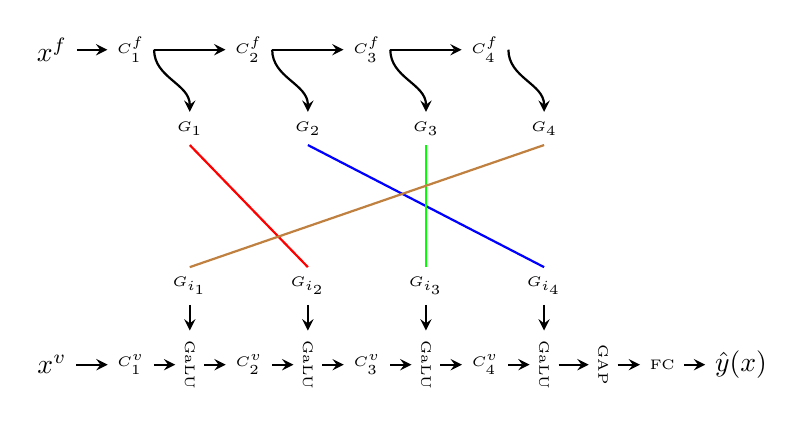
\begin{tikzpicture}
%\node []  (fntext)at (-4.625,-3.5) {CNN-GAP-DLGN};

%\node []  (output) at (7.5,1.5) {$\hat{y}(x)$};


\node [] (dgn1-f-c4) at (-3.5,1.5){\tiny{$C^{\text{f}}_4$}};
\node [] (dgn1-f-c3) at (-5,1.5){\tiny{$C^{\text{f}}_3$}};
\node [] (dgn1-f-c2) at (-6.5,1.5){\tiny{$C^{\text{f}}_2$}};
\node [] (dgn1-f-c1) at (-8,1.5){\tiny{$C^{\text{f}}_1$}};
\node [] (dgn1-input-f) at (-9,1.5){$x^{\text{f}}$};
\draw [-stealth,thick]   (dgn1-f-c3.east) -- (dgn1-f-c4.west);
\draw [-stealth,thick]   (dgn1-f-c2.east) -- (dgn1-f-c3.west);
\draw [-stealth,thick]   (dgn1-f-c1.east) -- (dgn1-f-c2.west);
\draw [-stealth,thick]   (dgn1-input-f.east) -- (dgn1-f-c1.west);



\node []  (dgn1-output) at (-0.25,-2.5) {$\hat{y}(x)$};

\node [] (dgn1-smax) at (-1.25,-2.5){\tiny{FC}};
\draw [-stealth,thick]   (dgn1-smax.east)--(dgn1-output.west);

\node [rotate=-90] (dgn1-gap) at (-2,-2.5){\tiny{GAP}};
\draw [-stealth,thick]   (dgn1-gap.north)--(dgn1-smax.west);


\node [rotate=-90] (dgn1-galu-4) at (-2.75,-2.5){\tiny{GaLU}};
\draw [-stealth,thick]   (dgn1-galu-4.north)--(dgn1-gap.south);

\node [] (dgn1-v-c4) at (-3.5,-2.5){\tiny{$C^{\text{v}}_4$}};
\draw [-stealth,thick]   (dgn1-v-c4.east) -- (dgn1-galu-4.south);


\node [rotate=-90] (dgn1-galu-3) at (-4.25,-2.5){\tiny{GaLU}};
\draw [-stealth,thick]   (dgn1-galu-3.north) -- (dgn1-v-c4.west);

\node [] (dgn1-v-c3) at (-5,-2.5){\tiny{$C^{\text{v}}_3$}};
\draw [-stealth,thick]   (dgn1-v-c3.east) -- (dgn1-galu-3.south);


\node [rotate=-90] (dgn1-galu-2) at (-5.75,-2.5){\tiny{GaLU}};
\draw [-stealth,thick]   (dgn1-galu-2.north) -- (dgn1-v-c3.west);

\node [] (dgn1-v-c2) at (-6.5,-2.5){\tiny{$C^{\text{v}}_2$}};
\draw [-stealth,thick]   (dgn1-v-c2.east) -- (dgn1-galu-2.south);


\node [rotate=-90] (dgn1-galu-1) at (-7.25,-2.5){\tiny{GaLU}};
\draw [-stealth,thick]   (dgn1-galu-1.north) -- (dgn1-v-c2.west);


\node [] (dgn1-v-c1) at (-8,-2.5){\tiny{$C^{\text{v}}_1$}};
\draw [-stealth,thick]   (dgn1-v-c1.east) -- (dgn1-galu-1.south);


\node [] (dgn1-v-input) at (-9,-2.5){$x^{\text{v}}$};

\draw [-stealth,thick]   (dgn1-v-input.east) -- (dgn1-v-c1.west);


\node[] (dgn1-gating-4-up) at (-2.75,0.5){\tiny{$G_{4}$}};
\draw [-stealth,thick]   (dgn1-f-c4.east) to[out=-90,in=90] (dgn1-gating-4-up.north);


\node[] (dgn1-gating-3-up) at (-4.25,0.5){\tiny{$G_{3}$}};
\draw [-stealth,thick]   (dgn1-f-c3.east) to[out=-90,in=90] (dgn1-gating-3-up.north);



\node[] (dgn1-gating-2-up) at (-5.75,0.5){\tiny{$G_{2}$}};
\draw [-stealth,thick]   (dgn1-f-c2.east) to[out=-90,in=90] (dgn1-gating-2-up.north);


\node[] (dgn1-gating-1-up) at (-7.25,0.5){\tiny{$G_{1}$}};
\draw [-stealth,thick]   (dgn1-f-c1.east) to[out=-90,in=90] (dgn1-gating-1-up.north);





\node[] (dgn1-gating-4) at (-2.75,-1.5){\tiny{$G_{i_4}$}};
\draw [-stealth,thick]   (dgn1-gating-4.south) -- (dgn1-galu-4.west);


\node[] (dgn1-gating-3) at (-4.25,-1.5){\tiny{$G_{i_3}$}};
\draw [-stealth,thick]   (dgn1-gating-3.south) -- (dgn1-galu-3.west);



\node[] (dgn1-gating-2) at (-5.75,-1.5){\tiny{$G_{i_2}$}};
\draw [-stealth,thick]   (dgn1-gating-2.south) -- (dgn1-galu-2.west);


\node[] (dgn1-gating-1) at (-7.25,-1.5){\tiny{$G_{i_1}$}};
\draw [-stealth,thick]   (dgn1-gating-1.south) -- (dgn1-galu-1.west);



\draw [-,thick,color=red]   (dgn1-gating-1-up.south) --(dgn1-gating-2.north);

\draw [-,thick,color=blue]   (dgn1-gating-2-up.south) --(dgn1-gating-4.north);

\draw [-,thick,color=green]   (dgn1-gating-3-up.south) --(dgn1-gating-3.north);

\draw [-,thick,color=brown]   (dgn1-gating-4-up.south) --(dgn1-gating-1.north);


%%%%%%%%%%%%%%%%%%%%%%%%%%%%%%%%%%%%%%%%%%%%%%%%%%%%%%%%%%%%%%%%%
	
\end{tikzpicture}


}
\end{minipage}

\begin{minipage}{0.48\columnwidth}
\centering
\resizebox{0.99\columnwidth}{!}{
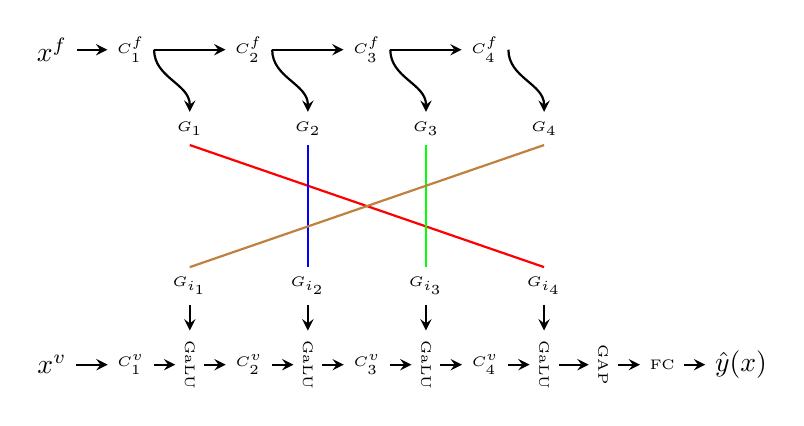
\begin{tikzpicture}
%\node []  (fntext)at (-4.625,-3.5) {CNN-GAP-DLGN};

%\node []  (output) at (7.5,1.5) {$\hat{y}(x)$};


\node [] (dgn1-f-c4) at (-3.5,1.5){\tiny{$C^{\text{f}}_4$}};
\node [] (dgn1-f-c3) at (-5,1.5){\tiny{$C^{\text{f}}_3$}};
\node [] (dgn1-f-c2) at (-6.5,1.5){\tiny{$C^{\text{f}}_2$}};
\node [] (dgn1-f-c1) at (-8,1.5){\tiny{$C^{\text{f}}_1$}};
\node [] (dgn1-input-f) at (-9,1.5){$x^{\text{f}}$};
\draw [-stealth,thick]   (dgn1-f-c3.east) -- (dgn1-f-c4.west);
\draw [-stealth,thick]   (dgn1-f-c2.east) -- (dgn1-f-c3.west);
\draw [-stealth,thick]   (dgn1-f-c1.east) -- (dgn1-f-c2.west);
\draw [-stealth,thick]   (dgn1-input-f.east) -- (dgn1-f-c1.west);



\node []  (dgn1-output) at (-0.25,-2.5) {$\hat{y}(x)$};

\node [] (dgn1-smax) at (-1.25,-2.5){\tiny{FC}};
\draw [-stealth,thick]   (dgn1-smax.east)--(dgn1-output.west);

\node [rotate=-90] (dgn1-gap) at (-2,-2.5){\tiny{GAP}};
\draw [-stealth,thick]   (dgn1-gap.north)--(dgn1-smax.west);


\node [rotate=-90] (dgn1-galu-4) at (-2.75,-2.5){\tiny{GaLU}};
\draw [-stealth,thick]   (dgn1-galu-4.north)--(dgn1-gap.south);

\node [] (dgn1-v-c4) at (-3.5,-2.5){\tiny{$C^{\text{v}}_4$}};
\draw [-stealth,thick]   (dgn1-v-c4.east) -- (dgn1-galu-4.south);


\node [rotate=-90] (dgn1-galu-3) at (-4.25,-2.5){\tiny{GaLU}};
\draw [-stealth,thick]   (dgn1-galu-3.north) -- (dgn1-v-c4.west);

\node [] (dgn1-v-c3) at (-5,-2.5){\tiny{$C^{\text{v}}_3$}};
\draw [-stealth,thick]   (dgn1-v-c3.east) -- (dgn1-galu-3.south);


\node [rotate=-90] (dgn1-galu-2) at (-5.75,-2.5){\tiny{GaLU}};
\draw [-stealth,thick]   (dgn1-galu-2.north) -- (dgn1-v-c3.west);

\node [] (dgn1-v-c2) at (-6.5,-2.5){\tiny{$C^{\text{v}}_2$}};
\draw [-stealth,thick]   (dgn1-v-c2.east) -- (dgn1-galu-2.south);


\node [rotate=-90] (dgn1-galu-1) at (-7.25,-2.5){\tiny{GaLU}};
\draw [-stealth,thick]   (dgn1-galu-1.north) -- (dgn1-v-c2.west);


\node [] (dgn1-v-c1) at (-8,-2.5){\tiny{$C^{\text{v}}_1$}};
\draw [-stealth,thick]   (dgn1-v-c1.east) -- (dgn1-galu-1.south);


\node [] (dgn1-v-input) at (-9,-2.5){$x^{\text{v}}$};

\draw [-stealth,thick]   (dgn1-v-input.east) -- (dgn1-v-c1.west);


\node[] (dgn1-gating-4-up) at (-2.75,0.5){\tiny{$G_{4}$}};
\draw [-stealth,thick]   (dgn1-f-c4.east) to[out=-90,in=90] (dgn1-gating-4-up.north);


\node[] (dgn1-gating-3-up) at (-4.25,0.5){\tiny{$G_{3}$}};
\draw [-stealth,thick]   (dgn1-f-c3.east) to[out=-90,in=90] (dgn1-gating-3-up.north);



\node[] (dgn1-gating-2-up) at (-5.75,0.5){\tiny{$G_{2}$}};
\draw [-stealth,thick]   (dgn1-f-c2.east) to[out=-90,in=90] (dgn1-gating-2-up.north);


\node[] (dgn1-gating-1-up) at (-7.25,0.5){\tiny{$G_{1}$}};
\draw [-stealth,thick]   (dgn1-f-c1.east) to[out=-90,in=90] (dgn1-gating-1-up.north);





\node[] (dgn1-gating-4) at (-2.75,-1.5){\tiny{$G_{i_4}$}};
\draw [-stealth,thick]   (dgn1-gating-4.south) -- (dgn1-galu-4.west);


\node[] (dgn1-gating-3) at (-4.25,-1.5){\tiny{$G_{i_3}$}};
\draw [-stealth,thick]   (dgn1-gating-3.south) -- (dgn1-galu-3.west);



\node[] (dgn1-gating-2) at (-5.75,-1.5){\tiny{$G_{i_2}$}};
\draw [-stealth,thick]   (dgn1-gating-2.south) -- (dgn1-galu-2.west);


\node[] (dgn1-gating-1) at (-7.25,-1.5){\tiny{$G_{i_1}$}};
\draw [-stealth,thick]   (dgn1-gating-1.south) -- (dgn1-galu-1.west);



\draw [-,thick,color=red]   (dgn1-gating-1-up.south) --(dgn1-gating-4.north);

\draw [-,thick,color=blue]   (dgn1-gating-2-up.south) --(dgn1-gating-2.north);

\draw [-,thick,color=green]   (dgn1-gating-3-up.south) --(dgn1-gating-3.north);

\draw [-,thick,color=brown]   (dgn1-gating-4-up.south) --(dgn1-gating-1.north);


%%%%%%%%%%%%%%%%%%%%%%%%%%%%%%%%%%%%%%%%%%%%%%%%%%%%%%%%%%%%%%%%%
	
\end{tikzpicture}


}
\end{minipage}
\begin{minipage}{0.48\columnwidth}
\centering
\resizebox{0.99\columnwidth}{!}{
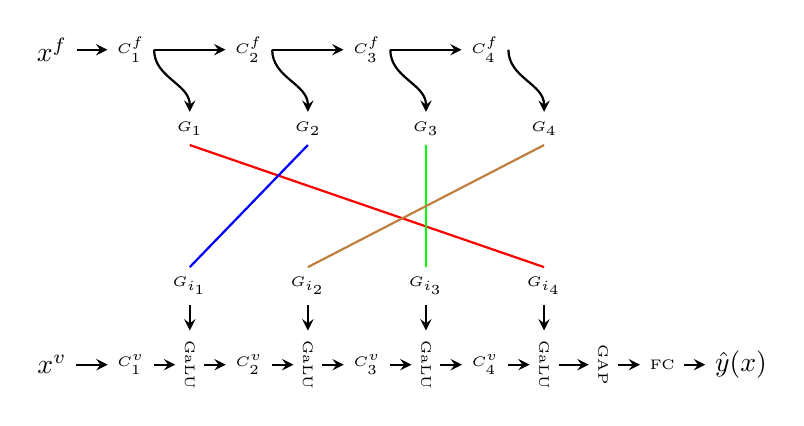
\begin{tikzpicture}
%\node []  (fntext)at (-4.625,-3.5) {CNN-GAP-DLGN};

%\node []  (output) at (7.5,1.5) {$\hat{y}(x)$};


\node [] (dgn1-f-c4) at (-3.5,1.5){\tiny{$C^{\text{f}}_4$}};
\node [] (dgn1-f-c3) at (-5,1.5){\tiny{$C^{\text{f}}_3$}};
\node [] (dgn1-f-c2) at (-6.5,1.5){\tiny{$C^{\text{f}}_2$}};
\node [] (dgn1-f-c1) at (-8,1.5){\tiny{$C^{\text{f}}_1$}};
\node [] (dgn1-input-f) at (-9,1.5){$x^{\text{f}}$};
\draw [-stealth,thick]   (dgn1-f-c3.east) -- (dgn1-f-c4.west);
\draw [-stealth,thick]   (dgn1-f-c2.east) -- (dgn1-f-c3.west);
\draw [-stealth,thick]   (dgn1-f-c1.east) -- (dgn1-f-c2.west);
\draw [-stealth,thick]   (dgn1-input-f.east) -- (dgn1-f-c1.west);



\node []  (dgn1-output) at (-0.25,-2.5) {$\hat{y}(x)$};

\node [] (dgn1-smax) at (-1.25,-2.5){\tiny{FC}};
\draw [-stealth,thick]   (dgn1-smax.east)--(dgn1-output.west);

\node [rotate=-90] (dgn1-gap) at (-2,-2.5){\tiny{GAP}};
\draw [-stealth,thick]   (dgn1-gap.north)--(dgn1-smax.west);


\node [rotate=-90] (dgn1-galu-4) at (-2.75,-2.5){\tiny{GaLU}};
\draw [-stealth,thick]   (dgn1-galu-4.north)--(dgn1-gap.south);

\node [] (dgn1-v-c4) at (-3.5,-2.5){\tiny{$C^{\text{v}}_4$}};
\draw [-stealth,thick]   (dgn1-v-c4.east) -- (dgn1-galu-4.south);


\node [rotate=-90] (dgn1-galu-3) at (-4.25,-2.5){\tiny{GaLU}};
\draw [-stealth,thick]   (dgn1-galu-3.north) -- (dgn1-v-c4.west);

\node [] (dgn1-v-c3) at (-5,-2.5){\tiny{$C^{\text{v}}_3$}};
\draw [-stealth,thick]   (dgn1-v-c3.east) -- (dgn1-galu-3.south);


\node [rotate=-90] (dgn1-galu-2) at (-5.75,-2.5){\tiny{GaLU}};
\draw [-stealth,thick]   (dgn1-galu-2.north) -- (dgn1-v-c3.west);

\node [] (dgn1-v-c2) at (-6.5,-2.5){\tiny{$C^{\text{v}}_2$}};
\draw [-stealth,thick]   (dgn1-v-c2.east) -- (dgn1-galu-2.south);


\node [rotate=-90] (dgn1-galu-1) at (-7.25,-2.5){\tiny{GaLU}};
\draw [-stealth,thick]   (dgn1-galu-1.north) -- (dgn1-v-c2.west);


\node [] (dgn1-v-c1) at (-8,-2.5){\tiny{$C^{\text{v}}_1$}};
\draw [-stealth,thick]   (dgn1-v-c1.east) -- (dgn1-galu-1.south);


\node [] (dgn1-v-input) at (-9,-2.5){$x^{\text{v}}$};

\draw [-stealth,thick]   (dgn1-v-input.east) -- (dgn1-v-c1.west);


\node[] (dgn1-gating-4-up) at (-2.75,0.5){\tiny{$G_{4}$}};
\draw [-stealth,thick]   (dgn1-f-c4.east) to[out=-90,in=90] (dgn1-gating-4-up.north);


\node[] (dgn1-gating-3-up) at (-4.25,0.5){\tiny{$G_{3}$}};
\draw [-stealth,thick]   (dgn1-f-c3.east) to[out=-90,in=90] (dgn1-gating-3-up.north);



\node[] (dgn1-gating-2-up) at (-5.75,0.5){\tiny{$G_{2}$}};
\draw [-stealth,thick]   (dgn1-f-c2.east) to[out=-90,in=90] (dgn1-gating-2-up.north);


\node[] (dgn1-gating-1-up) at (-7.25,0.5){\tiny{$G_{1}$}};
\draw [-stealth,thick]   (dgn1-f-c1.east) to[out=-90,in=90] (dgn1-gating-1-up.north);





\node[] (dgn1-gating-4) at (-2.75,-1.5){\tiny{$G_{i_4}$}};
\draw [-stealth,thick]   (dgn1-gating-4.south) -- (dgn1-galu-4.west);


\node[] (dgn1-gating-3) at (-4.25,-1.5){\tiny{$G_{i_3}$}};
\draw [-stealth,thick]   (dgn1-gating-3.south) -- (dgn1-galu-3.west);



\node[] (dgn1-gating-2) at (-5.75,-1.5){\tiny{$G_{i_2}$}};
\draw [-stealth,thick]   (dgn1-gating-2.south) -- (dgn1-galu-2.west);


\node[] (dgn1-gating-1) at (-7.25,-1.5){\tiny{$G_{i_1}$}};
\draw [-stealth,thick]   (dgn1-gating-1.south) -- (dgn1-galu-1.west);



\draw [-,thick,color=red]   (dgn1-gating-1-up.south) --(dgn1-gating-4.north);

\draw [-,thick,color=blue]   (dgn1-gating-2-up.south) --(dgn1-gating-1.north);

\draw [-,thick,color=green]   (dgn1-gating-3-up.south) --(dgn1-gating-3.north);

\draw [-,thick,color=brown]   (dgn1-gating-4-up.south) --(dgn1-gating-2.north);


%%%%%%%%%%%%%%%%%%%%%%%%%%%%%%%%%%%%%%%%%%%%%%%%%%%%%%%%%%%%%%%%%
	
\end{tikzpicture}


}
\end{minipage}


\end{figure}

\begin{figure}
\centering
\begin{minipage}{0.48\columnwidth}
\centering
\resizebox{0.99\columnwidth}{!}{
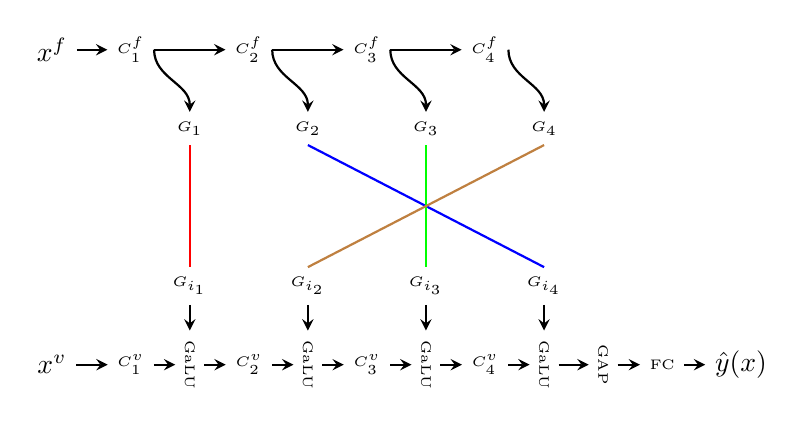
\begin{tikzpicture}
%\node []  (fntext)at (-4.625,-3.5) {CNN-GAP-DLGN};

%\node []  (output) at (7.5,1.5) {$\hat{y}(x)$};


\node [] (dgn1-f-c4) at (-3.5,1.5){\tiny{$C^{\text{f}}_4$}};
\node [] (dgn1-f-c3) at (-5,1.5){\tiny{$C^{\text{f}}_3$}};
\node [] (dgn1-f-c2) at (-6.5,1.5){\tiny{$C^{\text{f}}_2$}};
\node [] (dgn1-f-c1) at (-8,1.5){\tiny{$C^{\text{f}}_1$}};
\node [] (dgn1-input-f) at (-9,1.5){$x^{\text{f}}$};
\draw [-stealth,thick]   (dgn1-f-c3.east) -- (dgn1-f-c4.west);
\draw [-stealth,thick]   (dgn1-f-c2.east) -- (dgn1-f-c3.west);
\draw [-stealth,thick]   (dgn1-f-c1.east) -- (dgn1-f-c2.west);
\draw [-stealth,thick]   (dgn1-input-f.east) -- (dgn1-f-c1.west);



\node []  (dgn1-output) at (-0.25,-2.5) {$\hat{y}(x)$};

\node [] (dgn1-smax) at (-1.25,-2.5){\tiny{FC}};
\draw [-stealth,thick]   (dgn1-smax.east)--(dgn1-output.west);

\node [rotate=-90] (dgn1-gap) at (-2,-2.5){\tiny{GAP}};
\draw [-stealth,thick]   (dgn1-gap.north)--(dgn1-smax.west);


\node [rotate=-90] (dgn1-galu-4) at (-2.75,-2.5){\tiny{GaLU}};
\draw [-stealth,thick]   (dgn1-galu-4.north)--(dgn1-gap.south);

\node [] (dgn1-v-c4) at (-3.5,-2.5){\tiny{$C^{\text{v}}_4$}};
\draw [-stealth,thick]   (dgn1-v-c4.east) -- (dgn1-galu-4.south);


\node [rotate=-90] (dgn1-galu-3) at (-4.25,-2.5){\tiny{GaLU}};
\draw [-stealth,thick]   (dgn1-galu-3.north) -- (dgn1-v-c4.west);

\node [] (dgn1-v-c3) at (-5,-2.5){\tiny{$C^{\text{v}}_3$}};
\draw [-stealth,thick]   (dgn1-v-c3.east) -- (dgn1-galu-3.south);


\node [rotate=-90] (dgn1-galu-2) at (-5.75,-2.5){\tiny{GaLU}};
\draw [-stealth,thick]   (dgn1-galu-2.north) -- (dgn1-v-c3.west);

\node [] (dgn1-v-c2) at (-6.5,-2.5){\tiny{$C^{\text{v}}_2$}};
\draw [-stealth,thick]   (dgn1-v-c2.east) -- (dgn1-galu-2.south);


\node [rotate=-90] (dgn1-galu-1) at (-7.25,-2.5){\tiny{GaLU}};
\draw [-stealth,thick]   (dgn1-galu-1.north) -- (dgn1-v-c2.west);


\node [] (dgn1-v-c1) at (-8,-2.5){\tiny{$C^{\text{v}}_1$}};
\draw [-stealth,thick]   (dgn1-v-c1.east) -- (dgn1-galu-1.south);


\node [] (dgn1-v-input) at (-9,-2.5){$x^{\text{v}}$};

\draw [-stealth,thick]   (dgn1-v-input.east) -- (dgn1-v-c1.west);


\node[] (dgn1-gating-4-up) at (-2.75,0.5){\tiny{$G_{4}$}};
\draw [-stealth,thick]   (dgn1-f-c4.east) to[out=-90,in=90] (dgn1-gating-4-up.north);


\node[] (dgn1-gating-3-up) at (-4.25,0.5){\tiny{$G_{3}$}};
\draw [-stealth,thick]   (dgn1-f-c3.east) to[out=-90,in=90] (dgn1-gating-3-up.north);



\node[] (dgn1-gating-2-up) at (-5.75,0.5){\tiny{$G_{2}$}};
\draw [-stealth,thick]   (dgn1-f-c2.east) to[out=-90,in=90] (dgn1-gating-2-up.north);


\node[] (dgn1-gating-1-up) at (-7.25,0.5){\tiny{$G_{1}$}};
\draw [-stealth,thick]   (dgn1-f-c1.east) to[out=-90,in=90] (dgn1-gating-1-up.north);





\node[] (dgn1-gating-4) at (-2.75,-1.5){\tiny{$G_{i_4}$}};
\draw [-stealth,thick]   (dgn1-gating-4.south) -- (dgn1-galu-4.west);


\node[] (dgn1-gating-3) at (-4.25,-1.5){\tiny{$G_{i_3}$}};
\draw [-stealth,thick]   (dgn1-gating-3.south) -- (dgn1-galu-3.west);



\node[] (dgn1-gating-2) at (-5.75,-1.5){\tiny{$G_{i_2}$}};
\draw [-stealth,thick]   (dgn1-gating-2.south) -- (dgn1-galu-2.west);


\node[] (dgn1-gating-1) at (-7.25,-1.5){\tiny{$G_{i_1}$}};
\draw [-stealth,thick]   (dgn1-gating-1.south) -- (dgn1-galu-1.west);



\draw [-,thick,color=red]   (dgn1-gating-1-up.south) --(dgn1-gating-1.north);

\draw [-,thick,color=blue]   (dgn1-gating-2-up.south) --(dgn1-gating-4.north);

\draw [-,thick,color=green]   (dgn1-gating-3-up.south) --(dgn1-gating-3.north);

\draw [-,thick,color=brown]   (dgn1-gating-4-up.south) --(dgn1-gating-2.north);


%%%%%%%%%%%%%%%%%%%%%%%%%%%%%%%%%%%%%%%%%%%%%%%%%%%%%%%%%%%%%%%%%
	
\end{tikzpicture}


}
\end{minipage}
\begin{minipage}{0.48\columnwidth}
\centering
\resizebox{0.99\columnwidth}{!}{
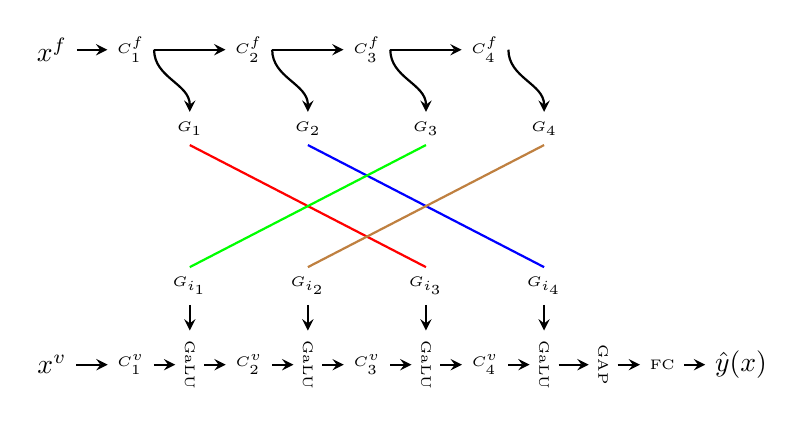
\begin{tikzpicture}
%\node []  (fntext)at (-4.625,-3.5) {CNN-GAP-DLGN};

%\node []  (output) at (7.5,1.5) {$\hat{y}(x)$};


\node [] (dgn1-f-c4) at (-3.5,1.5){\tiny{$C^{\text{f}}_4$}};
\node [] (dgn1-f-c3) at (-5,1.5){\tiny{$C^{\text{f}}_3$}};
\node [] (dgn1-f-c2) at (-6.5,1.5){\tiny{$C^{\text{f}}_2$}};
\node [] (dgn1-f-c1) at (-8,1.5){\tiny{$C^{\text{f}}_1$}};
\node [] (dgn1-input-f) at (-9,1.5){$x^{\text{f}}$};
\draw [-stealth,thick]   (dgn1-f-c3.east) -- (dgn1-f-c4.west);
\draw [-stealth,thick]   (dgn1-f-c2.east) -- (dgn1-f-c3.west);
\draw [-stealth,thick]   (dgn1-f-c1.east) -- (dgn1-f-c2.west);
\draw [-stealth,thick]   (dgn1-input-f.east) -- (dgn1-f-c1.west);



\node []  (dgn1-output) at (-0.25,-2.5) {$\hat{y}(x)$};

\node [] (dgn1-smax) at (-1.25,-2.5){\tiny{FC}};
\draw [-stealth,thick]   (dgn1-smax.east)--(dgn1-output.west);

\node [rotate=-90] (dgn1-gap) at (-2,-2.5){\tiny{GAP}};
\draw [-stealth,thick]   (dgn1-gap.north)--(dgn1-smax.west);


\node [rotate=-90] (dgn1-galu-4) at (-2.75,-2.5){\tiny{GaLU}};
\draw [-stealth,thick]   (dgn1-galu-4.north)--(dgn1-gap.south);

\node [] (dgn1-v-c4) at (-3.5,-2.5){\tiny{$C^{\text{v}}_4$}};
\draw [-stealth,thick]   (dgn1-v-c4.east) -- (dgn1-galu-4.south);


\node [rotate=-90] (dgn1-galu-3) at (-4.25,-2.5){\tiny{GaLU}};
\draw [-stealth,thick]   (dgn1-galu-3.north) -- (dgn1-v-c4.west);

\node [] (dgn1-v-c3) at (-5,-2.5){\tiny{$C^{\text{v}}_3$}};
\draw [-stealth,thick]   (dgn1-v-c3.east) -- (dgn1-galu-3.south);


\node [rotate=-90] (dgn1-galu-2) at (-5.75,-2.5){\tiny{GaLU}};
\draw [-stealth,thick]   (dgn1-galu-2.north) -- (dgn1-v-c3.west);

\node [] (dgn1-v-c2) at (-6.5,-2.5){\tiny{$C^{\text{v}}_2$}};
\draw [-stealth,thick]   (dgn1-v-c2.east) -- (dgn1-galu-2.south);


\node [rotate=-90] (dgn1-galu-1) at (-7.25,-2.5){\tiny{GaLU}};
\draw [-stealth,thick]   (dgn1-galu-1.north) -- (dgn1-v-c2.west);


\node [] (dgn1-v-c1) at (-8,-2.5){\tiny{$C^{\text{v}}_1$}};
\draw [-stealth,thick]   (dgn1-v-c1.east) -- (dgn1-galu-1.south);


\node [] (dgn1-v-input) at (-9,-2.5){$x^{\text{v}}$};

\draw [-stealth,thick]   (dgn1-v-input.east) -- (dgn1-v-c1.west);


\node[] (dgn1-gating-4-up) at (-2.75,0.5){\tiny{$G_{4}$}};
\draw [-stealth,thick]   (dgn1-f-c4.east) to[out=-90,in=90] (dgn1-gating-4-up.north);


\node[] (dgn1-gating-3-up) at (-4.25,0.5){\tiny{$G_{3}$}};
\draw [-stealth,thick]   (dgn1-f-c3.east) to[out=-90,in=90] (dgn1-gating-3-up.north);



\node[] (dgn1-gating-2-up) at (-5.75,0.5){\tiny{$G_{2}$}};
\draw [-stealth,thick]   (dgn1-f-c2.east) to[out=-90,in=90] (dgn1-gating-2-up.north);


\node[] (dgn1-gating-1-up) at (-7.25,0.5){\tiny{$G_{1}$}};
\draw [-stealth,thick]   (dgn1-f-c1.east) to[out=-90,in=90] (dgn1-gating-1-up.north);





\node[] (dgn1-gating-4) at (-2.75,-1.5){\tiny{$G_{i_4}$}};
\draw [-stealth,thick]   (dgn1-gating-4.south) -- (dgn1-galu-4.west);


\node[] (dgn1-gating-3) at (-4.25,-1.5){\tiny{$G_{i_3}$}};
\draw [-stealth,thick]   (dgn1-gating-3.south) -- (dgn1-galu-3.west);



\node[] (dgn1-gating-2) at (-5.75,-1.5){\tiny{$G_{i_2}$}};
\draw [-stealth,thick]   (dgn1-gating-2.south) -- (dgn1-galu-2.west);


\node[] (dgn1-gating-1) at (-7.25,-1.5){\tiny{$G_{i_1}$}};
\draw [-stealth,thick]   (dgn1-gating-1.south) -- (dgn1-galu-1.west);



\draw [-,thick,color=red]   (dgn1-gating-1-up.south) --(dgn1-gating-3.north);

\draw [-,thick,color=blue]   (dgn1-gating-2-up.south) --(dgn1-gating-4.north);

\draw [-,thick,color=green]   (dgn1-gating-3-up.south) --(dgn1-gating-1.north);

\draw [-,thick,color=brown]   (dgn1-gating-4-up.south) --(dgn1-gating-2.north);


%%%%%%%%%%%%%%%%%%%%%%%%%%%%%%%%%%%%%%%%%%%%%%%%%%%%%%%%%%%%%%%%%
	
\end{tikzpicture}


}
\end{minipage}

\begin{minipage}{0.48\columnwidth}
\centering
\resizebox{0.99\columnwidth}{!}{
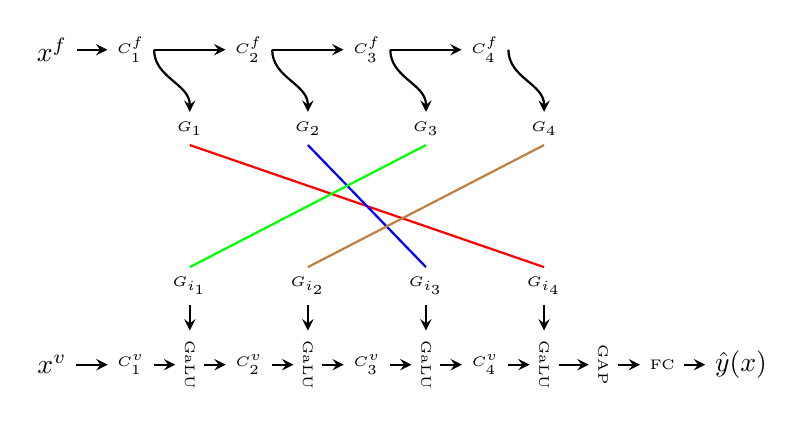
\begin{tikzpicture}
%\node []  (fntext)at (-4.625,-3.5) {CNN-GAP-DLGN};

%\node []  (output) at (7.5,1.5) {$\hat{y}(x)$};


\node [] (dgn1-f-c4) at (-3.5,1.5){\tiny{$C^{\text{f}}_4$}};
\node [] (dgn1-f-c3) at (-5,1.5){\tiny{$C^{\text{f}}_3$}};
\node [] (dgn1-f-c2) at (-6.5,1.5){\tiny{$C^{\text{f}}_2$}};
\node [] (dgn1-f-c1) at (-8,1.5){\tiny{$C^{\text{f}}_1$}};
\node [] (dgn1-input-f) at (-9,1.5){$x^{\text{f}}$};
\draw [-stealth,thick]   (dgn1-f-c3.east) -- (dgn1-f-c4.west);
\draw [-stealth,thick]   (dgn1-f-c2.east) -- (dgn1-f-c3.west);
\draw [-stealth,thick]   (dgn1-f-c1.east) -- (dgn1-f-c2.west);
\draw [-stealth,thick]   (dgn1-input-f.east) -- (dgn1-f-c1.west);



\node []  (dgn1-output) at (-0.25,-2.5) {$\hat{y}(x)$};

\node [] (dgn1-smax) at (-1.25,-2.5){\tiny{FC}};
\draw [-stealth,thick]   (dgn1-smax.east)--(dgn1-output.west);

\node [rotate=-90] (dgn1-gap) at (-2,-2.5){\tiny{GAP}};
\draw [-stealth,thick]   (dgn1-gap.north)--(dgn1-smax.west);


\node [rotate=-90] (dgn1-galu-4) at (-2.75,-2.5){\tiny{GaLU}};
\draw [-stealth,thick]   (dgn1-galu-4.north)--(dgn1-gap.south);

\node [] (dgn1-v-c4) at (-3.5,-2.5){\tiny{$C^{\text{v}}_4$}};
\draw [-stealth,thick]   (dgn1-v-c4.east) -- (dgn1-galu-4.south);


\node [rotate=-90] (dgn1-galu-3) at (-4.25,-2.5){\tiny{GaLU}};
\draw [-stealth,thick]   (dgn1-galu-3.north) -- (dgn1-v-c4.west);

\node [] (dgn1-v-c3) at (-5,-2.5){\tiny{$C^{\text{v}}_3$}};
\draw [-stealth,thick]   (dgn1-v-c3.east) -- (dgn1-galu-3.south);


\node [rotate=-90] (dgn1-galu-2) at (-5.75,-2.5){\tiny{GaLU}};
\draw [-stealth,thick]   (dgn1-galu-2.north) -- (dgn1-v-c3.west);

\node [] (dgn1-v-c2) at (-6.5,-2.5){\tiny{$C^{\text{v}}_2$}};
\draw [-stealth,thick]   (dgn1-v-c2.east) -- (dgn1-galu-2.south);


\node [rotate=-90] (dgn1-galu-1) at (-7.25,-2.5){\tiny{GaLU}};
\draw [-stealth,thick]   (dgn1-galu-1.north) -- (dgn1-v-c2.west);


\node [] (dgn1-v-c1) at (-8,-2.5){\tiny{$C^{\text{v}}_1$}};
\draw [-stealth,thick]   (dgn1-v-c1.east) -- (dgn1-galu-1.south);


\node [] (dgn1-v-input) at (-9,-2.5){$x^{\text{v}}$};

\draw [-stealth,thick]   (dgn1-v-input.east) -- (dgn1-v-c1.west);


\node[] (dgn1-gating-4-up) at (-2.75,0.5){\tiny{$G_{4}$}};
\draw [-stealth,thick]   (dgn1-f-c4.east) to[out=-90,in=90] (dgn1-gating-4-up.north);


\node[] (dgn1-gating-3-up) at (-4.25,0.5){\tiny{$G_{3}$}};
\draw [-stealth,thick]   (dgn1-f-c3.east) to[out=-90,in=90] (dgn1-gating-3-up.north);



\node[] (dgn1-gating-2-up) at (-5.75,0.5){\tiny{$G_{2}$}};
\draw [-stealth,thick]   (dgn1-f-c2.east) to[out=-90,in=90] (dgn1-gating-2-up.north);


\node[] (dgn1-gating-1-up) at (-7.25,0.5){\tiny{$G_{1}$}};
\draw [-stealth,thick]   (dgn1-f-c1.east) to[out=-90,in=90] (dgn1-gating-1-up.north);





\node[] (dgn1-gating-4) at (-2.75,-1.5){\tiny{$G_{i_4}$}};
\draw [-stealth,thick]   (dgn1-gating-4.south) -- (dgn1-galu-4.west);


\node[] (dgn1-gating-3) at (-4.25,-1.5){\tiny{$G_{i_3}$}};
\draw [-stealth,thick]   (dgn1-gating-3.south) -- (dgn1-galu-3.west);



\node[] (dgn1-gating-2) at (-5.75,-1.5){\tiny{$G_{i_2}$}};
\draw [-stealth,thick]   (dgn1-gating-2.south) -- (dgn1-galu-2.west);


\node[] (dgn1-gating-1) at (-7.25,-1.5){\tiny{$G_{i_1}$}};
\draw [-stealth,thick]   (dgn1-gating-1.south) -- (dgn1-galu-1.west);



\draw [-,thick,color=red]   (dgn1-gating-1-up.south) --(dgn1-gating-4.north);

\draw [-,thick,color=blue]   (dgn1-gating-2-up.south) --(dgn1-gating-3.north);

\draw [-,thick,color=green]   (dgn1-gating-3-up.south) --(dgn1-gating-1.north);

\draw [-,thick,color=brown]   (dgn1-gating-4-up.south) --(dgn1-gating-2.north);


%%%%%%%%%%%%%%%%%%%%%%%%%%%%%%%%%%%%%%%%%%%%%%%%%%%%%%%%%%%%%%%%%
	
\end{tikzpicture}


}
\end{minipage}
\begin{minipage}{0.48\columnwidth}
\centering
\resizebox{0.99\columnwidth}{!}{
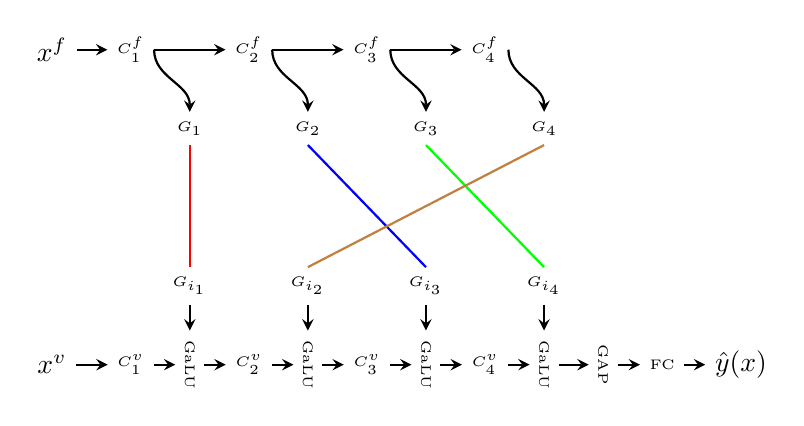
\begin{tikzpicture}
%\node []  (fntext)at (-4.625,-3.5) {CNN-GAP-DLGN};

%\node []  (output) at (7.5,1.5) {$\hat{y}(x)$};


\node [] (dgn1-f-c4) at (-3.5,1.5){\tiny{$C^{\text{f}}_4$}};
\node [] (dgn1-f-c3) at (-5,1.5){\tiny{$C^{\text{f}}_3$}};
\node [] (dgn1-f-c2) at (-6.5,1.5){\tiny{$C^{\text{f}}_2$}};
\node [] (dgn1-f-c1) at (-8,1.5){\tiny{$C^{\text{f}}_1$}};
\node [] (dgn1-input-f) at (-9,1.5){$x^{\text{f}}$};
\draw [-stealth,thick]   (dgn1-f-c3.east) -- (dgn1-f-c4.west);
\draw [-stealth,thick]   (dgn1-f-c2.east) -- (dgn1-f-c3.west);
\draw [-stealth,thick]   (dgn1-f-c1.east) -- (dgn1-f-c2.west);
\draw [-stealth,thick]   (dgn1-input-f.east) -- (dgn1-f-c1.west);



\node []  (dgn1-output) at (-0.25,-2.5) {$\hat{y}(x)$};

\node [] (dgn1-smax) at (-1.25,-2.5){\tiny{FC}};
\draw [-stealth,thick]   (dgn1-smax.east)--(dgn1-output.west);

\node [rotate=-90] (dgn1-gap) at (-2,-2.5){\tiny{GAP}};
\draw [-stealth,thick]   (dgn1-gap.north)--(dgn1-smax.west);


\node [rotate=-90] (dgn1-galu-4) at (-2.75,-2.5){\tiny{GaLU}};
\draw [-stealth,thick]   (dgn1-galu-4.north)--(dgn1-gap.south);

\node [] (dgn1-v-c4) at (-3.5,-2.5){\tiny{$C^{\text{v}}_4$}};
\draw [-stealth,thick]   (dgn1-v-c4.east) -- (dgn1-galu-4.south);


\node [rotate=-90] (dgn1-galu-3) at (-4.25,-2.5){\tiny{GaLU}};
\draw [-stealth,thick]   (dgn1-galu-3.north) -- (dgn1-v-c4.west);

\node [] (dgn1-v-c3) at (-5,-2.5){\tiny{$C^{\text{v}}_3$}};
\draw [-stealth,thick]   (dgn1-v-c3.east) -- (dgn1-galu-3.south);


\node [rotate=-90] (dgn1-galu-2) at (-5.75,-2.5){\tiny{GaLU}};
\draw [-stealth,thick]   (dgn1-galu-2.north) -- (dgn1-v-c3.west);

\node [] (dgn1-v-c2) at (-6.5,-2.5){\tiny{$C^{\text{v}}_2$}};
\draw [-stealth,thick]   (dgn1-v-c2.east) -- (dgn1-galu-2.south);


\node [rotate=-90] (dgn1-galu-1) at (-7.25,-2.5){\tiny{GaLU}};
\draw [-stealth,thick]   (dgn1-galu-1.north) -- (dgn1-v-c2.west);


\node [] (dgn1-v-c1) at (-8,-2.5){\tiny{$C^{\text{v}}_1$}};
\draw [-stealth,thick]   (dgn1-v-c1.east) -- (dgn1-galu-1.south);


\node [] (dgn1-v-input) at (-9,-2.5){$x^{\text{v}}$};

\draw [-stealth,thick]   (dgn1-v-input.east) -- (dgn1-v-c1.west);


\node[] (dgn1-gating-4-up) at (-2.75,0.5){\tiny{$G_{4}$}};
\draw [-stealth,thick]   (dgn1-f-c4.east) to[out=-90,in=90] (dgn1-gating-4-up.north);


\node[] (dgn1-gating-3-up) at (-4.25,0.5){\tiny{$G_{3}$}};
\draw [-stealth,thick]   (dgn1-f-c3.east) to[out=-90,in=90] (dgn1-gating-3-up.north);



\node[] (dgn1-gating-2-up) at (-5.75,0.5){\tiny{$G_{2}$}};
\draw [-stealth,thick]   (dgn1-f-c2.east) to[out=-90,in=90] (dgn1-gating-2-up.north);


\node[] (dgn1-gating-1-up) at (-7.25,0.5){\tiny{$G_{1}$}};
\draw [-stealth,thick]   (dgn1-f-c1.east) to[out=-90,in=90] (dgn1-gating-1-up.north);





\node[] (dgn1-gating-4) at (-2.75,-1.5){\tiny{$G_{i_4}$}};
\draw [-stealth,thick]   (dgn1-gating-4.south) -- (dgn1-galu-4.west);


\node[] (dgn1-gating-3) at (-4.25,-1.5){\tiny{$G_{i_3}$}};
\draw [-stealth,thick]   (dgn1-gating-3.south) -- (dgn1-galu-3.west);



\node[] (dgn1-gating-2) at (-5.75,-1.5){\tiny{$G_{i_2}$}};
\draw [-stealth,thick]   (dgn1-gating-2.south) -- (dgn1-galu-2.west);


\node[] (dgn1-gating-1) at (-7.25,-1.5){\tiny{$G_{i_1}$}};
\draw [-stealth,thick]   (dgn1-gating-1.south) -- (dgn1-galu-1.west);



\draw [-,thick,color=red]   (dgn1-gating-1-up.south) --(dgn1-gating-1.north);

\draw [-,thick,color=blue]   (dgn1-gating-2-up.south) --(dgn1-gating-3.north);

\draw [-,thick,color=green]   (dgn1-gating-3-up.south) --(dgn1-gating-4.north);

\draw [-,thick,color=brown]   (dgn1-gating-4-up.south) --(dgn1-gating-2.north);


%%%%%%%%%%%%%%%%%%%%%%%%%%%%%%%%%%%%%%%%%%%%%%%%%%%%%%%%%%%%%%%%%
	
\end{tikzpicture}


}
\end{minipage}


\begin{minipage}{0.48\columnwidth}
\centering
\resizebox{0.99\columnwidth}{!}{
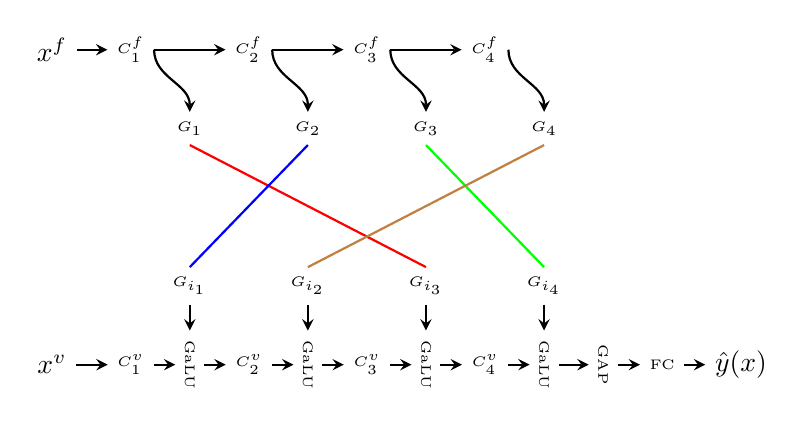
\begin{tikzpicture}
%\node []  (fntext)at (-4.625,-3.5) {CNN-GAP-DLGN};

%\node []  (output) at (7.5,1.5) {$\hat{y}(x)$};


\node [] (dgn1-f-c4) at (-3.5,1.5){\tiny{$C^{\text{f}}_4$}};
\node [] (dgn1-f-c3) at (-5,1.5){\tiny{$C^{\text{f}}_3$}};
\node [] (dgn1-f-c2) at (-6.5,1.5){\tiny{$C^{\text{f}}_2$}};
\node [] (dgn1-f-c1) at (-8,1.5){\tiny{$C^{\text{f}}_1$}};
\node [] (dgn1-input-f) at (-9,1.5){$x^{\text{f}}$};
\draw [-stealth,thick]   (dgn1-f-c3.east) -- (dgn1-f-c4.west);
\draw [-stealth,thick]   (dgn1-f-c2.east) -- (dgn1-f-c3.west);
\draw [-stealth,thick]   (dgn1-f-c1.east) -- (dgn1-f-c2.west);
\draw [-stealth,thick]   (dgn1-input-f.east) -- (dgn1-f-c1.west);



\node []  (dgn1-output) at (-0.25,-2.5) {$\hat{y}(x)$};

\node [] (dgn1-smax) at (-1.25,-2.5){\tiny{FC}};
\draw [-stealth,thick]   (dgn1-smax.east)--(dgn1-output.west);

\node [rotate=-90] (dgn1-gap) at (-2,-2.5){\tiny{GAP}};
\draw [-stealth,thick]   (dgn1-gap.north)--(dgn1-smax.west);


\node [rotate=-90] (dgn1-galu-4) at (-2.75,-2.5){\tiny{GaLU}};
\draw [-stealth,thick]   (dgn1-galu-4.north)--(dgn1-gap.south);

\node [] (dgn1-v-c4) at (-3.5,-2.5){\tiny{$C^{\text{v}}_4$}};
\draw [-stealth,thick]   (dgn1-v-c4.east) -- (dgn1-galu-4.south);


\node [rotate=-90] (dgn1-galu-3) at (-4.25,-2.5){\tiny{GaLU}};
\draw [-stealth,thick]   (dgn1-galu-3.north) -- (dgn1-v-c4.west);

\node [] (dgn1-v-c3) at (-5,-2.5){\tiny{$C^{\text{v}}_3$}};
\draw [-stealth,thick]   (dgn1-v-c3.east) -- (dgn1-galu-3.south);


\node [rotate=-90] (dgn1-galu-2) at (-5.75,-2.5){\tiny{GaLU}};
\draw [-stealth,thick]   (dgn1-galu-2.north) -- (dgn1-v-c3.west);

\node [] (dgn1-v-c2) at (-6.5,-2.5){\tiny{$C^{\text{v}}_2$}};
\draw [-stealth,thick]   (dgn1-v-c2.east) -- (dgn1-galu-2.south);


\node [rotate=-90] (dgn1-galu-1) at (-7.25,-2.5){\tiny{GaLU}};
\draw [-stealth,thick]   (dgn1-galu-1.north) -- (dgn1-v-c2.west);


\node [] (dgn1-v-c1) at (-8,-2.5){\tiny{$C^{\text{v}}_1$}};
\draw [-stealth,thick]   (dgn1-v-c1.east) -- (dgn1-galu-1.south);


\node [] (dgn1-v-input) at (-9,-2.5){$x^{\text{v}}$};

\draw [-stealth,thick]   (dgn1-v-input.east) -- (dgn1-v-c1.west);


\node[] (dgn1-gating-4-up) at (-2.75,0.5){\tiny{$G_{4}$}};
\draw [-stealth,thick]   (dgn1-f-c4.east) to[out=-90,in=90] (dgn1-gating-4-up.north);


\node[] (dgn1-gating-3-up) at (-4.25,0.5){\tiny{$G_{3}$}};
\draw [-stealth,thick]   (dgn1-f-c3.east) to[out=-90,in=90] (dgn1-gating-3-up.north);



\node[] (dgn1-gating-2-up) at (-5.75,0.5){\tiny{$G_{2}$}};
\draw [-stealth,thick]   (dgn1-f-c2.east) to[out=-90,in=90] (dgn1-gating-2-up.north);


\node[] (dgn1-gating-1-up) at (-7.25,0.5){\tiny{$G_{1}$}};
\draw [-stealth,thick]   (dgn1-f-c1.east) to[out=-90,in=90] (dgn1-gating-1-up.north);





\node[] (dgn1-gating-4) at (-2.75,-1.5){\tiny{$G_{i_4}$}};
\draw [-stealth,thick]   (dgn1-gating-4.south) -- (dgn1-galu-4.west);


\node[] (dgn1-gating-3) at (-4.25,-1.5){\tiny{$G_{i_3}$}};
\draw [-stealth,thick]   (dgn1-gating-3.south) -- (dgn1-galu-3.west);



\node[] (dgn1-gating-2) at (-5.75,-1.5){\tiny{$G_{i_2}$}};
\draw [-stealth,thick]   (dgn1-gating-2.south) -- (dgn1-galu-2.west);


\node[] (dgn1-gating-1) at (-7.25,-1.5){\tiny{$G_{i_1}$}};
\draw [-stealth,thick]   (dgn1-gating-1.south) -- (dgn1-galu-1.west);



\draw [-,thick,color=red]   (dgn1-gating-1-up.south) --(dgn1-gating-3.north);

\draw [-,thick,color=blue]   (dgn1-gating-2-up.south) --(dgn1-gating-1.north);

\draw [-,thick,color=green]   (dgn1-gating-3-up.south) --(dgn1-gating-4.north);

\draw [-,thick,color=brown]   (dgn1-gating-4-up.south) --(dgn1-gating-2.north);


%%%%%%%%%%%%%%%%%%%%%%%%%%%%%%%%%%%%%%%%%%%%%%%%%%%%%%%%%%%%%%%%%
	
\end{tikzpicture}


}
\end{minipage}
\begin{minipage}{0.48\columnwidth}
\centering
\resizebox{0.99\columnwidth}{!}{
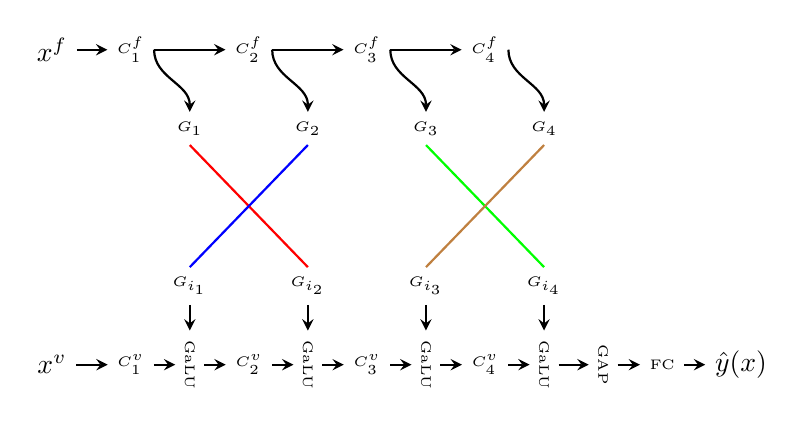
\begin{tikzpicture}
%\node []  (fntext)at (-4.625,-3.5) {CNN-GAP-DLGN};

%\node []  (output) at (7.5,1.5) {$\hat{y}(x)$};


\node [] (dgn1-f-c4) at (-3.5,1.5){\tiny{$C^{\text{f}}_4$}};
\node [] (dgn1-f-c3) at (-5,1.5){\tiny{$C^{\text{f}}_3$}};
\node [] (dgn1-f-c2) at (-6.5,1.5){\tiny{$C^{\text{f}}_2$}};
\node [] (dgn1-f-c1) at (-8,1.5){\tiny{$C^{\text{f}}_1$}};
\node [] (dgn1-input-f) at (-9,1.5){$x^{\text{f}}$};
\draw [-stealth,thick]   (dgn1-f-c3.east) -- (dgn1-f-c4.west);
\draw [-stealth,thick]   (dgn1-f-c2.east) -- (dgn1-f-c3.west);
\draw [-stealth,thick]   (dgn1-f-c1.east) -- (dgn1-f-c2.west);
\draw [-stealth,thick]   (dgn1-input-f.east) -- (dgn1-f-c1.west);



\node []  (dgn1-output) at (-0.25,-2.5) {$\hat{y}(x)$};

\node [] (dgn1-smax) at (-1.25,-2.5){\tiny{FC}};
\draw [-stealth,thick]   (dgn1-smax.east)--(dgn1-output.west);

\node [rotate=-90] (dgn1-gap) at (-2,-2.5){\tiny{GAP}};
\draw [-stealth,thick]   (dgn1-gap.north)--(dgn1-smax.west);


\node [rotate=-90] (dgn1-galu-4) at (-2.75,-2.5){\tiny{GaLU}};
\draw [-stealth,thick]   (dgn1-galu-4.north)--(dgn1-gap.south);

\node [] (dgn1-v-c4) at (-3.5,-2.5){\tiny{$C^{\text{v}}_4$}};
\draw [-stealth,thick]   (dgn1-v-c4.east) -- (dgn1-galu-4.south);


\node [rotate=-90] (dgn1-galu-3) at (-4.25,-2.5){\tiny{GaLU}};
\draw [-stealth,thick]   (dgn1-galu-3.north) -- (dgn1-v-c4.west);

\node [] (dgn1-v-c3) at (-5,-2.5){\tiny{$C^{\text{v}}_3$}};
\draw [-stealth,thick]   (dgn1-v-c3.east) -- (dgn1-galu-3.south);


\node [rotate=-90] (dgn1-galu-2) at (-5.75,-2.5){\tiny{GaLU}};
\draw [-stealth,thick]   (dgn1-galu-2.north) -- (dgn1-v-c3.west);

\node [] (dgn1-v-c2) at (-6.5,-2.5){\tiny{$C^{\text{v}}_2$}};
\draw [-stealth,thick]   (dgn1-v-c2.east) -- (dgn1-galu-2.south);


\node [rotate=-90] (dgn1-galu-1) at (-7.25,-2.5){\tiny{GaLU}};
\draw [-stealth,thick]   (dgn1-galu-1.north) -- (dgn1-v-c2.west);


\node [] (dgn1-v-c1) at (-8,-2.5){\tiny{$C^{\text{v}}_1$}};
\draw [-stealth,thick]   (dgn1-v-c1.east) -- (dgn1-galu-1.south);


\node [] (dgn1-v-input) at (-9,-2.5){$x^{\text{v}}$};

\draw [-stealth,thick]   (dgn1-v-input.east) -- (dgn1-v-c1.west);


\node[] (dgn1-gating-4-up) at (-2.75,0.5){\tiny{$G_{4}$}};
\draw [-stealth,thick]   (dgn1-f-c4.east) to[out=-90,in=90] (dgn1-gating-4-up.north);


\node[] (dgn1-gating-3-up) at (-4.25,0.5){\tiny{$G_{3}$}};
\draw [-stealth,thick]   (dgn1-f-c3.east) to[out=-90,in=90] (dgn1-gating-3-up.north);



\node[] (dgn1-gating-2-up) at (-5.75,0.5){\tiny{$G_{2}$}};
\draw [-stealth,thick]   (dgn1-f-c2.east) to[out=-90,in=90] (dgn1-gating-2-up.north);


\node[] (dgn1-gating-1-up) at (-7.25,0.5){\tiny{$G_{1}$}};
\draw [-stealth,thick]   (dgn1-f-c1.east) to[out=-90,in=90] (dgn1-gating-1-up.north);





\node[] (dgn1-gating-4) at (-2.75,-1.5){\tiny{$G_{i_4}$}};
\draw [-stealth,thick]   (dgn1-gating-4.south) -- (dgn1-galu-4.west);


\node[] (dgn1-gating-3) at (-4.25,-1.5){\tiny{$G_{i_3}$}};
\draw [-stealth,thick]   (dgn1-gating-3.south) -- (dgn1-galu-3.west);



\node[] (dgn1-gating-2) at (-5.75,-1.5){\tiny{$G_{i_2}$}};
\draw [-stealth,thick]   (dgn1-gating-2.south) -- (dgn1-galu-2.west);


\node[] (dgn1-gating-1) at (-7.25,-1.5){\tiny{$G_{i_1}$}};
\draw [-stealth,thick]   (dgn1-gating-1.south) -- (dgn1-galu-1.west);



\draw [-,thick,color=red]   (dgn1-gating-1-up.south) --(dgn1-gating-2.north);

\draw [-,thick,color=blue]   (dgn1-gating-2-up.south) --(dgn1-gating-1.north);

\draw [-,thick,color=green]   (dgn1-gating-3-up.south) --(dgn1-gating-4.north);

\draw [-,thick,color=brown]   (dgn1-gating-4-up.south) --(dgn1-gating-3.north);


%%%%%%%%%%%%%%%%%%%%%%%%%%%%%%%%%%%%%%%%%%%%%%%%%%%%%%%%%%%%%%%%%
	
\end{tikzpicture}


}
\end{minipage}



\begin{minipage}{0.48\columnwidth}
\centering
\resizebox{0.99\columnwidth}{!}{
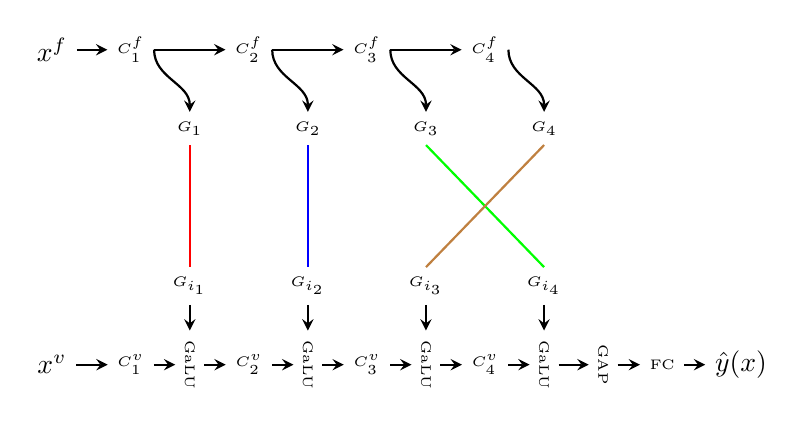
\begin{tikzpicture}
%\node []  (fntext)at (-4.625,-3.5) {CNN-GAP-DLGN};

%\node []  (output) at (7.5,1.5) {$\hat{y}(x)$};


\node [] (dgn1-f-c4) at (-3.5,1.5){\tiny{$C^{\text{f}}_4$}};
\node [] (dgn1-f-c3) at (-5,1.5){\tiny{$C^{\text{f}}_3$}};
\node [] (dgn1-f-c2) at (-6.5,1.5){\tiny{$C^{\text{f}}_2$}};
\node [] (dgn1-f-c1) at (-8,1.5){\tiny{$C^{\text{f}}_1$}};
\node [] (dgn1-input-f) at (-9,1.5){$x^{\text{f}}$};
\draw [-stealth,thick]   (dgn1-f-c3.east) -- (dgn1-f-c4.west);
\draw [-stealth,thick]   (dgn1-f-c2.east) -- (dgn1-f-c3.west);
\draw [-stealth,thick]   (dgn1-f-c1.east) -- (dgn1-f-c2.west);
\draw [-stealth,thick]   (dgn1-input-f.east) -- (dgn1-f-c1.west);



\node []  (dgn1-output) at (-0.25,-2.5) {$\hat{y}(x)$};

\node [] (dgn1-smax) at (-1.25,-2.5){\tiny{FC}};
\draw [-stealth,thick]   (dgn1-smax.east)--(dgn1-output.west);

\node [rotate=-90] (dgn1-gap) at (-2,-2.5){\tiny{GAP}};
\draw [-stealth,thick]   (dgn1-gap.north)--(dgn1-smax.west);


\node [rotate=-90] (dgn1-galu-4) at (-2.75,-2.5){\tiny{GaLU}};
\draw [-stealth,thick]   (dgn1-galu-4.north)--(dgn1-gap.south);

\node [] (dgn1-v-c4) at (-3.5,-2.5){\tiny{$C^{\text{v}}_4$}};
\draw [-stealth,thick]   (dgn1-v-c4.east) -- (dgn1-galu-4.south);


\node [rotate=-90] (dgn1-galu-3) at (-4.25,-2.5){\tiny{GaLU}};
\draw [-stealth,thick]   (dgn1-galu-3.north) -- (dgn1-v-c4.west);

\node [] (dgn1-v-c3) at (-5,-2.5){\tiny{$C^{\text{v}}_3$}};
\draw [-stealth,thick]   (dgn1-v-c3.east) -- (dgn1-galu-3.south);


\node [rotate=-90] (dgn1-galu-2) at (-5.75,-2.5){\tiny{GaLU}};
\draw [-stealth,thick]   (dgn1-galu-2.north) -- (dgn1-v-c3.west);

\node [] (dgn1-v-c2) at (-6.5,-2.5){\tiny{$C^{\text{v}}_2$}};
\draw [-stealth,thick]   (dgn1-v-c2.east) -- (dgn1-galu-2.south);


\node [rotate=-90] (dgn1-galu-1) at (-7.25,-2.5){\tiny{GaLU}};
\draw [-stealth,thick]   (dgn1-galu-1.north) -- (dgn1-v-c2.west);


\node [] (dgn1-v-c1) at (-8,-2.5){\tiny{$C^{\text{v}}_1$}};
\draw [-stealth,thick]   (dgn1-v-c1.east) -- (dgn1-galu-1.south);


\node [] (dgn1-v-input) at (-9,-2.5){$x^{\text{v}}$};

\draw [-stealth,thick]   (dgn1-v-input.east) -- (dgn1-v-c1.west);


\node[] (dgn1-gating-4-up) at (-2.75,0.5){\tiny{$G_{4}$}};
\draw [-stealth,thick]   (dgn1-f-c4.east) to[out=-90,in=90] (dgn1-gating-4-up.north);


\node[] (dgn1-gating-3-up) at (-4.25,0.5){\tiny{$G_{3}$}};
\draw [-stealth,thick]   (dgn1-f-c3.east) to[out=-90,in=90] (dgn1-gating-3-up.north);



\node[] (dgn1-gating-2-up) at (-5.75,0.5){\tiny{$G_{2}$}};
\draw [-stealth,thick]   (dgn1-f-c2.east) to[out=-90,in=90] (dgn1-gating-2-up.north);


\node[] (dgn1-gating-1-up) at (-7.25,0.5){\tiny{$G_{1}$}};
\draw [-stealth,thick]   (dgn1-f-c1.east) to[out=-90,in=90] (dgn1-gating-1-up.north);





\node[] (dgn1-gating-4) at (-2.75,-1.5){\tiny{$G_{i_4}$}};
\draw [-stealth,thick]   (dgn1-gating-4.south) -- (dgn1-galu-4.west);


\node[] (dgn1-gating-3) at (-4.25,-1.5){\tiny{$G_{i_3}$}};
\draw [-stealth,thick]   (dgn1-gating-3.south) -- (dgn1-galu-3.west);



\node[] (dgn1-gating-2) at (-5.75,-1.5){\tiny{$G_{i_2}$}};
\draw [-stealth,thick]   (dgn1-gating-2.south) -- (dgn1-galu-2.west);


\node[] (dgn1-gating-1) at (-7.25,-1.5){\tiny{$G_{i_1}$}};
\draw [-stealth,thick]   (dgn1-gating-1.south) -- (dgn1-galu-1.west);



\draw [-,thick,color=red]   (dgn1-gating-1-up.south) --(dgn1-gating-1.north);

\draw [-,thick,color=blue]   (dgn1-gating-2-up.south) --(dgn1-gating-2.north);

\draw [-,thick,color=green]   (dgn1-gating-3-up.south) --(dgn1-gating-4.north);

\draw [-,thick,color=brown]   (dgn1-gating-4-up.south) --(dgn1-gating-3.north);


%%%%%%%%%%%%%%%%%%%%%%%%%%%%%%%%%%%%%%%%%%%%%%%%%%%%%%%%%%%%%%%%%
	
\end{tikzpicture}


}
\end{minipage}
\begin{minipage}{0.48\columnwidth}
\centering
\resizebox{0.99\columnwidth}{!}{
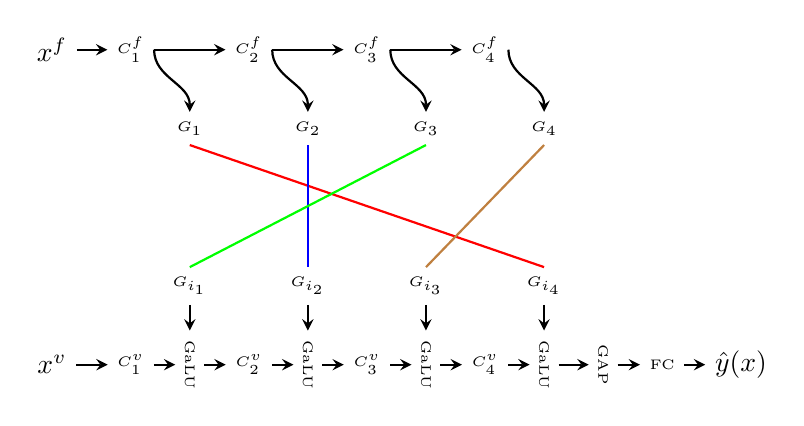
\begin{tikzpicture}
%\node []  (fntext)at (-4.625,-3.5) {CNN-GAP-DLGN};

%\node []  (output) at (7.5,1.5) {$\hat{y}(x)$};


\node [] (dgn1-f-c4) at (-3.5,1.5){\tiny{$C^{\text{f}}_4$}};
\node [] (dgn1-f-c3) at (-5,1.5){\tiny{$C^{\text{f}}_3$}};
\node [] (dgn1-f-c2) at (-6.5,1.5){\tiny{$C^{\text{f}}_2$}};
\node [] (dgn1-f-c1) at (-8,1.5){\tiny{$C^{\text{f}}_1$}};
\node [] (dgn1-input-f) at (-9,1.5){$x^{\text{f}}$};
\draw [-stealth,thick]   (dgn1-f-c3.east) -- (dgn1-f-c4.west);
\draw [-stealth,thick]   (dgn1-f-c2.east) -- (dgn1-f-c3.west);
\draw [-stealth,thick]   (dgn1-f-c1.east) -- (dgn1-f-c2.west);
\draw [-stealth,thick]   (dgn1-input-f.east) -- (dgn1-f-c1.west);



\node []  (dgn1-output) at (-0.25,-2.5) {$\hat{y}(x)$};

\node [] (dgn1-smax) at (-1.25,-2.5){\tiny{FC}};
\draw [-stealth,thick]   (dgn1-smax.east)--(dgn1-output.west);

\node [rotate=-90] (dgn1-gap) at (-2,-2.5){\tiny{GAP}};
\draw [-stealth,thick]   (dgn1-gap.north)--(dgn1-smax.west);


\node [rotate=-90] (dgn1-galu-4) at (-2.75,-2.5){\tiny{GaLU}};
\draw [-stealth,thick]   (dgn1-galu-4.north)--(dgn1-gap.south);

\node [] (dgn1-v-c4) at (-3.5,-2.5){\tiny{$C^{\text{v}}_4$}};
\draw [-stealth,thick]   (dgn1-v-c4.east) -- (dgn1-galu-4.south);


\node [rotate=-90] (dgn1-galu-3) at (-4.25,-2.5){\tiny{GaLU}};
\draw [-stealth,thick]   (dgn1-galu-3.north) -- (dgn1-v-c4.west);

\node [] (dgn1-v-c3) at (-5,-2.5){\tiny{$C^{\text{v}}_3$}};
\draw [-stealth,thick]   (dgn1-v-c3.east) -- (dgn1-galu-3.south);


\node [rotate=-90] (dgn1-galu-2) at (-5.75,-2.5){\tiny{GaLU}};
\draw [-stealth,thick]   (dgn1-galu-2.north) -- (dgn1-v-c3.west);

\node [] (dgn1-v-c2) at (-6.5,-2.5){\tiny{$C^{\text{v}}_2$}};
\draw [-stealth,thick]   (dgn1-v-c2.east) -- (dgn1-galu-2.south);


\node [rotate=-90] (dgn1-galu-1) at (-7.25,-2.5){\tiny{GaLU}};
\draw [-stealth,thick]   (dgn1-galu-1.north) -- (dgn1-v-c2.west);


\node [] (dgn1-v-c1) at (-8,-2.5){\tiny{$C^{\text{v}}_1$}};
\draw [-stealth,thick]   (dgn1-v-c1.east) -- (dgn1-galu-1.south);


\node [] (dgn1-v-input) at (-9,-2.5){$x^{\text{v}}$};

\draw [-stealth,thick]   (dgn1-v-input.east) -- (dgn1-v-c1.west);


\node[] (dgn1-gating-4-up) at (-2.75,0.5){\tiny{$G_{4}$}};
\draw [-stealth,thick]   (dgn1-f-c4.east) to[out=-90,in=90] (dgn1-gating-4-up.north);


\node[] (dgn1-gating-3-up) at (-4.25,0.5){\tiny{$G_{3}$}};
\draw [-stealth,thick]   (dgn1-f-c3.east) to[out=-90,in=90] (dgn1-gating-3-up.north);



\node[] (dgn1-gating-2-up) at (-5.75,0.5){\tiny{$G_{2}$}};
\draw [-stealth,thick]   (dgn1-f-c2.east) to[out=-90,in=90] (dgn1-gating-2-up.north);


\node[] (dgn1-gating-1-up) at (-7.25,0.5){\tiny{$G_{1}$}};
\draw [-stealth,thick]   (dgn1-f-c1.east) to[out=-90,in=90] (dgn1-gating-1-up.north);





\node[] (dgn1-gating-4) at (-2.75,-1.5){\tiny{$G_{i_4}$}};
\draw [-stealth,thick]   (dgn1-gating-4.south) -- (dgn1-galu-4.west);


\node[] (dgn1-gating-3) at (-4.25,-1.5){\tiny{$G_{i_3}$}};
\draw [-stealth,thick]   (dgn1-gating-3.south) -- (dgn1-galu-3.west);



\node[] (dgn1-gating-2) at (-5.75,-1.5){\tiny{$G_{i_2}$}};
\draw [-stealth,thick]   (dgn1-gating-2.south) -- (dgn1-galu-2.west);


\node[] (dgn1-gating-1) at (-7.25,-1.5){\tiny{$G_{i_1}$}};
\draw [-stealth,thick]   (dgn1-gating-1.south) -- (dgn1-galu-1.west);



\draw [-,thick,color=red]   (dgn1-gating-1-up.south) --(dgn1-gating-4.north);

\draw [-,thick,color=blue]   (dgn1-gating-2-up.south) --(dgn1-gating-2.north);

\draw [-,thick,color=green]   (dgn1-gating-3-up.south) --(dgn1-gating-1.north);

\draw [-,thick,color=brown]   (dgn1-gating-4-up.south) --(dgn1-gating-3.north);


%%%%%%%%%%%%%%%%%%%%%%%%%%%%%%%%%%%%%%%%%%%%%%%%%%%%%%%%%%%%%%%%%
	
\end{tikzpicture}


}
\end{minipage}

\begin{minipage}{0.48\columnwidth}
\centering
\resizebox{0.99\columnwidth}{!}{
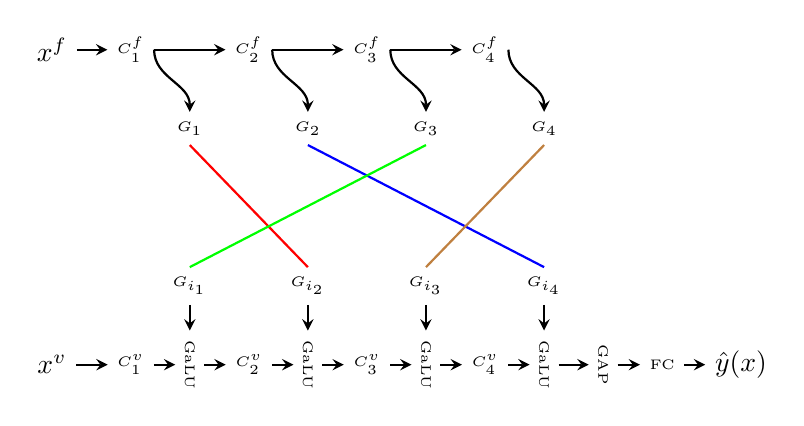
\begin{tikzpicture}
%\node []  (fntext)at (-4.625,-3.5) {CNN-GAP-DLGN};

%\node []  (output) at (7.5,1.5) {$\hat{y}(x)$};


\node [] (dgn1-f-c4) at (-3.5,1.5){\tiny{$C^{\text{f}}_4$}};
\node [] (dgn1-f-c3) at (-5,1.5){\tiny{$C^{\text{f}}_3$}};
\node [] (dgn1-f-c2) at (-6.5,1.5){\tiny{$C^{\text{f}}_2$}};
\node [] (dgn1-f-c1) at (-8,1.5){\tiny{$C^{\text{f}}_1$}};
\node [] (dgn1-input-f) at (-9,1.5){$x^{\text{f}}$};
\draw [-stealth,thick]   (dgn1-f-c3.east) -- (dgn1-f-c4.west);
\draw [-stealth,thick]   (dgn1-f-c2.east) -- (dgn1-f-c3.west);
\draw [-stealth,thick]   (dgn1-f-c1.east) -- (dgn1-f-c2.west);
\draw [-stealth,thick]   (dgn1-input-f.east) -- (dgn1-f-c1.west);



\node []  (dgn1-output) at (-0.25,-2.5) {$\hat{y}(x)$};

\node [] (dgn1-smax) at (-1.25,-2.5){\tiny{FC}};
\draw [-stealth,thick]   (dgn1-smax.east)--(dgn1-output.west);

\node [rotate=-90] (dgn1-gap) at (-2,-2.5){\tiny{GAP}};
\draw [-stealth,thick]   (dgn1-gap.north)--(dgn1-smax.west);


\node [rotate=-90] (dgn1-galu-4) at (-2.75,-2.5){\tiny{GaLU}};
\draw [-stealth,thick]   (dgn1-galu-4.north)--(dgn1-gap.south);

\node [] (dgn1-v-c4) at (-3.5,-2.5){\tiny{$C^{\text{v}}_4$}};
\draw [-stealth,thick]   (dgn1-v-c4.east) -- (dgn1-galu-4.south);


\node [rotate=-90] (dgn1-galu-3) at (-4.25,-2.5){\tiny{GaLU}};
\draw [-stealth,thick]   (dgn1-galu-3.north) -- (dgn1-v-c4.west);

\node [] (dgn1-v-c3) at (-5,-2.5){\tiny{$C^{\text{v}}_3$}};
\draw [-stealth,thick]   (dgn1-v-c3.east) -- (dgn1-galu-3.south);


\node [rotate=-90] (dgn1-galu-2) at (-5.75,-2.5){\tiny{GaLU}};
\draw [-stealth,thick]   (dgn1-galu-2.north) -- (dgn1-v-c3.west);

\node [] (dgn1-v-c2) at (-6.5,-2.5){\tiny{$C^{\text{v}}_2$}};
\draw [-stealth,thick]   (dgn1-v-c2.east) -- (dgn1-galu-2.south);


\node [rotate=-90] (dgn1-galu-1) at (-7.25,-2.5){\tiny{GaLU}};
\draw [-stealth,thick]   (dgn1-galu-1.north) -- (dgn1-v-c2.west);


\node [] (dgn1-v-c1) at (-8,-2.5){\tiny{$C^{\text{v}}_1$}};
\draw [-stealth,thick]   (dgn1-v-c1.east) -- (dgn1-galu-1.south);


\node [] (dgn1-v-input) at (-9,-2.5){$x^{\text{v}}$};

\draw [-stealth,thick]   (dgn1-v-input.east) -- (dgn1-v-c1.west);


\node[] (dgn1-gating-4-up) at (-2.75,0.5){\tiny{$G_{4}$}};
\draw [-stealth,thick]   (dgn1-f-c4.east) to[out=-90,in=90] (dgn1-gating-4-up.north);


\node[] (dgn1-gating-3-up) at (-4.25,0.5){\tiny{$G_{3}$}};
\draw [-stealth,thick]   (dgn1-f-c3.east) to[out=-90,in=90] (dgn1-gating-3-up.north);



\node[] (dgn1-gating-2-up) at (-5.75,0.5){\tiny{$G_{2}$}};
\draw [-stealth,thick]   (dgn1-f-c2.east) to[out=-90,in=90] (dgn1-gating-2-up.north);


\node[] (dgn1-gating-1-up) at (-7.25,0.5){\tiny{$G_{1}$}};
\draw [-stealth,thick]   (dgn1-f-c1.east) to[out=-90,in=90] (dgn1-gating-1-up.north);





\node[] (dgn1-gating-4) at (-2.75,-1.5){\tiny{$G_{i_4}$}};
\draw [-stealth,thick]   (dgn1-gating-4.south) -- (dgn1-galu-4.west);


\node[] (dgn1-gating-3) at (-4.25,-1.5){\tiny{$G_{i_3}$}};
\draw [-stealth,thick]   (dgn1-gating-3.south) -- (dgn1-galu-3.west);



\node[] (dgn1-gating-2) at (-5.75,-1.5){\tiny{$G_{i_2}$}};
\draw [-stealth,thick]   (dgn1-gating-2.south) -- (dgn1-galu-2.west);


\node[] (dgn1-gating-1) at (-7.25,-1.5){\tiny{$G_{i_1}$}};
\draw [-stealth,thick]   (dgn1-gating-1.south) -- (dgn1-galu-1.west);



\draw [-,thick,color=red]   (dgn1-gating-1-up.south) --(dgn1-gating-2.north);

\draw [-,thick,color=blue]   (dgn1-gating-2-up.south) --(dgn1-gating-4.north);

\draw [-,thick,color=green]   (dgn1-gating-3-up.south) --(dgn1-gating-1.north);

\draw [-,thick,color=brown]   (dgn1-gating-4-up.south) --(dgn1-gating-3.north);


%%%%%%%%%%%%%%%%%%%%%%%%%%%%%%%%%%%%%%%%%%%%%%%%%%%%%%%%%%%%%%%%%
	
\end{tikzpicture}


}
\end{minipage}
\begin{minipage}{0.48\columnwidth}
\centering
\resizebox{0.99\columnwidth}{!}{
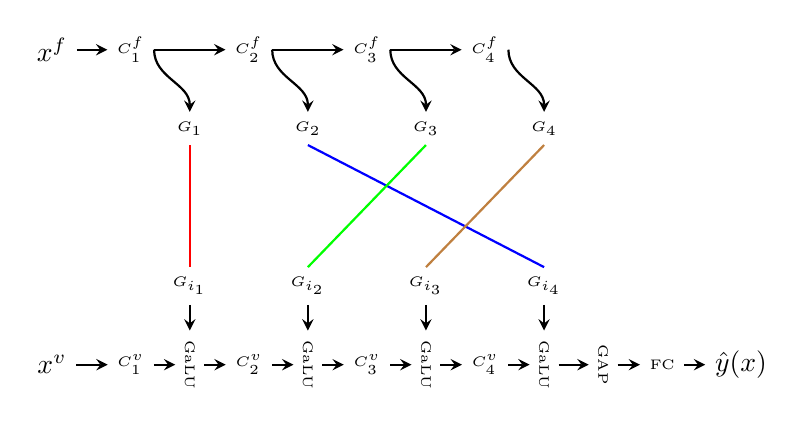
\begin{tikzpicture}
%\node []  (fntext)at (-4.625,-3.5) {CNN-GAP-DLGN};

%\node []  (output) at (7.5,1.5) {$\hat{y}(x)$};


\node [] (dgn1-f-c4) at (-3.5,1.5){\tiny{$C^{\text{f}}_4$}};
\node [] (dgn1-f-c3) at (-5,1.5){\tiny{$C^{\text{f}}_3$}};
\node [] (dgn1-f-c2) at (-6.5,1.5){\tiny{$C^{\text{f}}_2$}};
\node [] (dgn1-f-c1) at (-8,1.5){\tiny{$C^{\text{f}}_1$}};
\node [] (dgn1-input-f) at (-9,1.5){$x^{\text{f}}$};
\draw [-stealth,thick]   (dgn1-f-c3.east) -- (dgn1-f-c4.west);
\draw [-stealth,thick]   (dgn1-f-c2.east) -- (dgn1-f-c3.west);
\draw [-stealth,thick]   (dgn1-f-c1.east) -- (dgn1-f-c2.west);
\draw [-stealth,thick]   (dgn1-input-f.east) -- (dgn1-f-c1.west);



\node []  (dgn1-output) at (-0.25,-2.5) {$\hat{y}(x)$};

\node [] (dgn1-smax) at (-1.25,-2.5){\tiny{FC}};
\draw [-stealth,thick]   (dgn1-smax.east)--(dgn1-output.west);

\node [rotate=-90] (dgn1-gap) at (-2,-2.5){\tiny{GAP}};
\draw [-stealth,thick]   (dgn1-gap.north)--(dgn1-smax.west);


\node [rotate=-90] (dgn1-galu-4) at (-2.75,-2.5){\tiny{GaLU}};
\draw [-stealth,thick]   (dgn1-galu-4.north)--(dgn1-gap.south);

\node [] (dgn1-v-c4) at (-3.5,-2.5){\tiny{$C^{\text{v}}_4$}};
\draw [-stealth,thick]   (dgn1-v-c4.east) -- (dgn1-galu-4.south);


\node [rotate=-90] (dgn1-galu-3) at (-4.25,-2.5){\tiny{GaLU}};
\draw [-stealth,thick]   (dgn1-galu-3.north) -- (dgn1-v-c4.west);

\node [] (dgn1-v-c3) at (-5,-2.5){\tiny{$C^{\text{v}}_3$}};
\draw [-stealth,thick]   (dgn1-v-c3.east) -- (dgn1-galu-3.south);


\node [rotate=-90] (dgn1-galu-2) at (-5.75,-2.5){\tiny{GaLU}};
\draw [-stealth,thick]   (dgn1-galu-2.north) -- (dgn1-v-c3.west);

\node [] (dgn1-v-c2) at (-6.5,-2.5){\tiny{$C^{\text{v}}_2$}};
\draw [-stealth,thick]   (dgn1-v-c2.east) -- (dgn1-galu-2.south);


\node [rotate=-90] (dgn1-galu-1) at (-7.25,-2.5){\tiny{GaLU}};
\draw [-stealth,thick]   (dgn1-galu-1.north) -- (dgn1-v-c2.west);


\node [] (dgn1-v-c1) at (-8,-2.5){\tiny{$C^{\text{v}}_1$}};
\draw [-stealth,thick]   (dgn1-v-c1.east) -- (dgn1-galu-1.south);


\node [] (dgn1-v-input) at (-9,-2.5){$x^{\text{v}}$};

\draw [-stealth,thick]   (dgn1-v-input.east) -- (dgn1-v-c1.west);


\node[] (dgn1-gating-4-up) at (-2.75,0.5){\tiny{$G_{4}$}};
\draw [-stealth,thick]   (dgn1-f-c4.east) to[out=-90,in=90] (dgn1-gating-4-up.north);


\node[] (dgn1-gating-3-up) at (-4.25,0.5){\tiny{$G_{3}$}};
\draw [-stealth,thick]   (dgn1-f-c3.east) to[out=-90,in=90] (dgn1-gating-3-up.north);



\node[] (dgn1-gating-2-up) at (-5.75,0.5){\tiny{$G_{2}$}};
\draw [-stealth,thick]   (dgn1-f-c2.east) to[out=-90,in=90] (dgn1-gating-2-up.north);


\node[] (dgn1-gating-1-up) at (-7.25,0.5){\tiny{$G_{1}$}};
\draw [-stealth,thick]   (dgn1-f-c1.east) to[out=-90,in=90] (dgn1-gating-1-up.north);





\node[] (dgn1-gating-4) at (-2.75,-1.5){\tiny{$G_{i_4}$}};
\draw [-stealth,thick]   (dgn1-gating-4.south) -- (dgn1-galu-4.west);


\node[] (dgn1-gating-3) at (-4.25,-1.5){\tiny{$G_{i_3}$}};
\draw [-stealth,thick]   (dgn1-gating-3.south) -- (dgn1-galu-3.west);



\node[] (dgn1-gating-2) at (-5.75,-1.5){\tiny{$G_{i_2}$}};
\draw [-stealth,thick]   (dgn1-gating-2.south) -- (dgn1-galu-2.west);


\node[] (dgn1-gating-1) at (-7.25,-1.5){\tiny{$G_{i_1}$}};
\draw [-stealth,thick]   (dgn1-gating-1.south) -- (dgn1-galu-1.west);



\draw [-,thick,color=red]   (dgn1-gating-1-up.south) --(dgn1-gating-1.north);

\draw [-,thick,color=blue]   (dgn1-gating-2-up.south) --(dgn1-gating-4.north);

\draw [-,thick,color=green]   (dgn1-gating-3-up.south) --(dgn1-gating-2.north);

\draw [-,thick,color=brown]   (dgn1-gating-4-up.south) --(dgn1-gating-3.north);


%%%%%%%%%%%%%%%%%%%%%%%%%%%%%%%%%%%%%%%%%%%%%%%%%%%%%%%%%%%%%%%%%
	
\end{tikzpicture}


}
\end{minipage}

\begin{minipage}{0.48\columnwidth}
\centering
\resizebox{0.99\columnwidth}{!}{
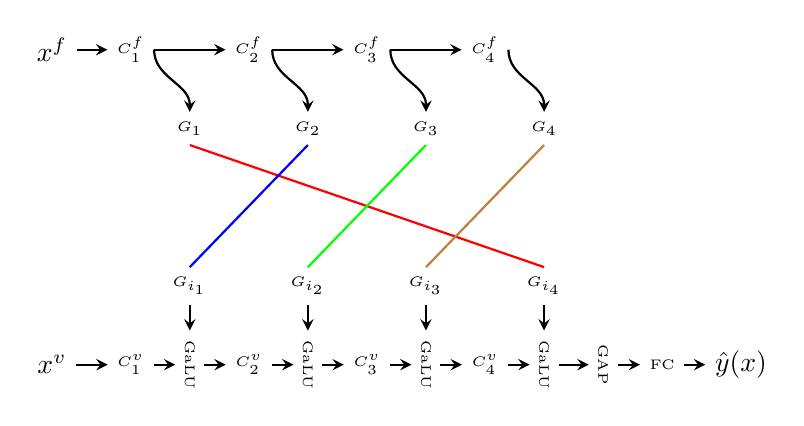
\begin{tikzpicture}
%\node []  (fntext)at (-4.625,-3.5) {CNN-GAP-DLGN};

%\node []  (output) at (7.5,1.5) {$\hat{y}(x)$};


\node [] (dgn1-f-c4) at (-3.5,1.5){\tiny{$C^{\text{f}}_4$}};
\node [] (dgn1-f-c3) at (-5,1.5){\tiny{$C^{\text{f}}_3$}};
\node [] (dgn1-f-c2) at (-6.5,1.5){\tiny{$C^{\text{f}}_2$}};
\node [] (dgn1-f-c1) at (-8,1.5){\tiny{$C^{\text{f}}_1$}};
\node [] (dgn1-input-f) at (-9,1.5){$x^{\text{f}}$};
\draw [-stealth,thick]   (dgn1-f-c3.east) -- (dgn1-f-c4.west);
\draw [-stealth,thick]   (dgn1-f-c2.east) -- (dgn1-f-c3.west);
\draw [-stealth,thick]   (dgn1-f-c1.east) -- (dgn1-f-c2.west);
\draw [-stealth,thick]   (dgn1-input-f.east) -- (dgn1-f-c1.west);



\node []  (dgn1-output) at (-0.25,-2.5) {$\hat{y}(x)$};

\node [] (dgn1-smax) at (-1.25,-2.5){\tiny{FC}};
\draw [-stealth,thick]   (dgn1-smax.east)--(dgn1-output.west);

\node [rotate=-90] (dgn1-gap) at (-2,-2.5){\tiny{GAP}};
\draw [-stealth,thick]   (dgn1-gap.north)--(dgn1-smax.west);


\node [rotate=-90] (dgn1-galu-4) at (-2.75,-2.5){\tiny{GaLU}};
\draw [-stealth,thick]   (dgn1-galu-4.north)--(dgn1-gap.south);

\node [] (dgn1-v-c4) at (-3.5,-2.5){\tiny{$C^{\text{v}}_4$}};
\draw [-stealth,thick]   (dgn1-v-c4.east) -- (dgn1-galu-4.south);


\node [rotate=-90] (dgn1-galu-3) at (-4.25,-2.5){\tiny{GaLU}};
\draw [-stealth,thick]   (dgn1-galu-3.north) -- (dgn1-v-c4.west);

\node [] (dgn1-v-c3) at (-5,-2.5){\tiny{$C^{\text{v}}_3$}};
\draw [-stealth,thick]   (dgn1-v-c3.east) -- (dgn1-galu-3.south);


\node [rotate=-90] (dgn1-galu-2) at (-5.75,-2.5){\tiny{GaLU}};
\draw [-stealth,thick]   (dgn1-galu-2.north) -- (dgn1-v-c3.west);

\node [] (dgn1-v-c2) at (-6.5,-2.5){\tiny{$C^{\text{v}}_2$}};
\draw [-stealth,thick]   (dgn1-v-c2.east) -- (dgn1-galu-2.south);


\node [rotate=-90] (dgn1-galu-1) at (-7.25,-2.5){\tiny{GaLU}};
\draw [-stealth,thick]   (dgn1-galu-1.north) -- (dgn1-v-c2.west);


\node [] (dgn1-v-c1) at (-8,-2.5){\tiny{$C^{\text{v}}_1$}};
\draw [-stealth,thick]   (dgn1-v-c1.east) -- (dgn1-galu-1.south);


\node [] (dgn1-v-input) at (-9,-2.5){$x^{\text{v}}$};

\draw [-stealth,thick]   (dgn1-v-input.east) -- (dgn1-v-c1.west);


\node[] (dgn1-gating-4-up) at (-2.75,0.5){\tiny{$G_{4}$}};
\draw [-stealth,thick]   (dgn1-f-c4.east) to[out=-90,in=90] (dgn1-gating-4-up.north);


\node[] (dgn1-gating-3-up) at (-4.25,0.5){\tiny{$G_{3}$}};
\draw [-stealth,thick]   (dgn1-f-c3.east) to[out=-90,in=90] (dgn1-gating-3-up.north);



\node[] (dgn1-gating-2-up) at (-5.75,0.5){\tiny{$G_{2}$}};
\draw [-stealth,thick]   (dgn1-f-c2.east) to[out=-90,in=90] (dgn1-gating-2-up.north);


\node[] (dgn1-gating-1-up) at (-7.25,0.5){\tiny{$G_{1}$}};
\draw [-stealth,thick]   (dgn1-f-c1.east) to[out=-90,in=90] (dgn1-gating-1-up.north);





\node[] (dgn1-gating-4) at (-2.75,-1.5){\tiny{$G_{i_4}$}};
\draw [-stealth,thick]   (dgn1-gating-4.south) -- (dgn1-galu-4.west);


\node[] (dgn1-gating-3) at (-4.25,-1.5){\tiny{$G_{i_3}$}};
\draw [-stealth,thick]   (dgn1-gating-3.south) -- (dgn1-galu-3.west);



\node[] (dgn1-gating-2) at (-5.75,-1.5){\tiny{$G_{i_2}$}};
\draw [-stealth,thick]   (dgn1-gating-2.south) -- (dgn1-galu-2.west);


\node[] (dgn1-gating-1) at (-7.25,-1.5){\tiny{$G_{i_1}$}};
\draw [-stealth,thick]   (dgn1-gating-1.south) -- (dgn1-galu-1.west);



\draw [-,thick,color=red]   (dgn1-gating-1-up.south) --(dgn1-gating-4.north);

\draw [-,thick,color=blue]   (dgn1-gating-2-up.south) --(dgn1-gating-1.north);

\draw [-,thick,color=green]   (dgn1-gating-3-up.south) --(dgn1-gating-2.north);

\draw [-,thick,color=brown]   (dgn1-gating-4-up.south) --(dgn1-gating-3.north);


%%%%%%%%%%%%%%%%%%%%%%%%%%%%%%%%%%%%%%%%%%%%%%%%%%%%%%%%%%%%%%%%%
	
\end{tikzpicture}


}
\end{minipage}
\begin{minipage}{0.48\columnwidth}
\centering
\resizebox{0.99\columnwidth}{!}{
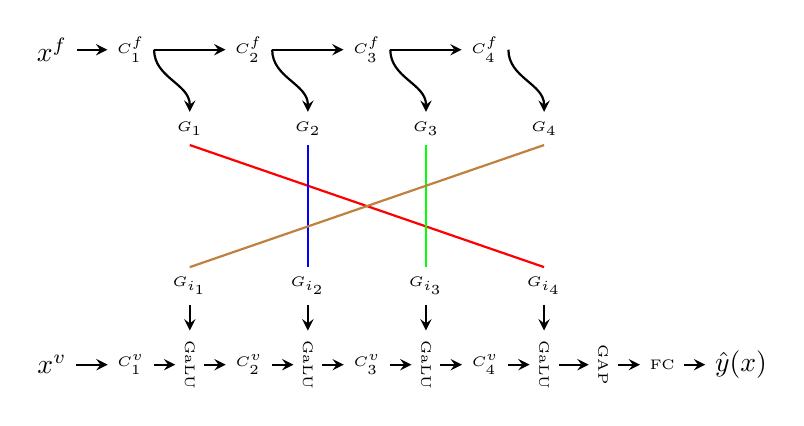
\begin{tikzpicture}
%\node []  (fntext)at (-4.625,-3.5) {CNN-GAP-DLGN};

%\node []  (output) at (7.5,1.5) {$\hat{y}(x)$};


\node [] (dgn1-f-c4) at (-3.5,1.5){\tiny{$C^{\text{f}}_4$}};
\node [] (dgn1-f-c3) at (-5,1.5){\tiny{$C^{\text{f}}_3$}};
\node [] (dgn1-f-c2) at (-6.5,1.5){\tiny{$C^{\text{f}}_2$}};
\node [] (dgn1-f-c1) at (-8,1.5){\tiny{$C^{\text{f}}_1$}};
\node [] (dgn1-input-f) at (-9,1.5){$x^{\text{f}}$};
\draw [-stealth,thick]   (dgn1-f-c3.east) -- (dgn1-f-c4.west);
\draw [-stealth,thick]   (dgn1-f-c2.east) -- (dgn1-f-c3.west);
\draw [-stealth,thick]   (dgn1-f-c1.east) -- (dgn1-f-c2.west);
\draw [-stealth,thick]   (dgn1-input-f.east) -- (dgn1-f-c1.west);



\node []  (dgn1-output) at (-0.25,-2.5) {$\hat{y}(x)$};

\node [] (dgn1-smax) at (-1.25,-2.5){\tiny{FC}};
\draw [-stealth,thick]   (dgn1-smax.east)--(dgn1-output.west);

\node [rotate=-90] (dgn1-gap) at (-2,-2.5){\tiny{GAP}};
\draw [-stealth,thick]   (dgn1-gap.north)--(dgn1-smax.west);


\node [rotate=-90] (dgn1-galu-4) at (-2.75,-2.5){\tiny{GaLU}};
\draw [-stealth,thick]   (dgn1-galu-4.north)--(dgn1-gap.south);

\node [] (dgn1-v-c4) at (-3.5,-2.5){\tiny{$C^{\text{v}}_4$}};
\draw [-stealth,thick]   (dgn1-v-c4.east) -- (dgn1-galu-4.south);


\node [rotate=-90] (dgn1-galu-3) at (-4.25,-2.5){\tiny{GaLU}};
\draw [-stealth,thick]   (dgn1-galu-3.north) -- (dgn1-v-c4.west);

\node [] (dgn1-v-c3) at (-5,-2.5){\tiny{$C^{\text{v}}_3$}};
\draw [-stealth,thick]   (dgn1-v-c3.east) -- (dgn1-galu-3.south);


\node [rotate=-90] (dgn1-galu-2) at (-5.75,-2.5){\tiny{GaLU}};
\draw [-stealth,thick]   (dgn1-galu-2.north) -- (dgn1-v-c3.west);

\node [] (dgn1-v-c2) at (-6.5,-2.5){\tiny{$C^{\text{v}}_2$}};
\draw [-stealth,thick]   (dgn1-v-c2.east) -- (dgn1-galu-2.south);


\node [rotate=-90] (dgn1-galu-1) at (-7.25,-2.5){\tiny{GaLU}};
\draw [-stealth,thick]   (dgn1-galu-1.north) -- (dgn1-v-c2.west);


\node [] (dgn1-v-c1) at (-8,-2.5){\tiny{$C^{\text{v}}_1$}};
\draw [-stealth,thick]   (dgn1-v-c1.east) -- (dgn1-galu-1.south);


\node [] (dgn1-v-input) at (-9,-2.5){$x^{\text{v}}$};

\draw [-stealth,thick]   (dgn1-v-input.east) -- (dgn1-v-c1.west);


\node[] (dgn1-gating-4-up) at (-2.75,0.5){\tiny{$G_{4}$}};
\draw [-stealth,thick]   (dgn1-f-c4.east) to[out=-90,in=90] (dgn1-gating-4-up.north);


\node[] (dgn1-gating-3-up) at (-4.25,0.5){\tiny{$G_{3}$}};
\draw [-stealth,thick]   (dgn1-f-c3.east) to[out=-90,in=90] (dgn1-gating-3-up.north);



\node[] (dgn1-gating-2-up) at (-5.75,0.5){\tiny{$G_{2}$}};
\draw [-stealth,thick]   (dgn1-f-c2.east) to[out=-90,in=90] (dgn1-gating-2-up.north);


\node[] (dgn1-gating-1-up) at (-7.25,0.5){\tiny{$G_{1}$}};
\draw [-stealth,thick]   (dgn1-f-c1.east) to[out=-90,in=90] (dgn1-gating-1-up.north);





\node[] (dgn1-gating-4) at (-2.75,-1.5){\tiny{$G_{i_4}$}};
\draw [-stealth,thick]   (dgn1-gating-4.south) -- (dgn1-galu-4.west);


\node[] (dgn1-gating-3) at (-4.25,-1.5){\tiny{$G_{i_3}$}};
\draw [-stealth,thick]   (dgn1-gating-3.south) -- (dgn1-galu-3.west);



\node[] (dgn1-gating-2) at (-5.75,-1.5){\tiny{$G_{i_2}$}};
\draw [-stealth,thick]   (dgn1-gating-2.south) -- (dgn1-galu-2.west);


\node[] (dgn1-gating-1) at (-7.25,-1.5){\tiny{$G_{i_1}$}};
\draw [-stealth,thick]   (dgn1-gating-1.south) -- (dgn1-galu-1.west);



\draw [-,thick,color=red]   (dgn1-gating-1-up.south) --(dgn1-gating-4.north);

\draw [-,thick,color=blue]   (dgn1-gating-2-up.south) --(dgn1-gating-2.north);

\draw [-,thick,color=green]   (dgn1-gating-3-up.south) --(dgn1-gating-3.north);

\draw [-,thick,color=brown]   (dgn1-gating-4-up.south) --(dgn1-gating-1.north);


%%%%%%%%%%%%%%%%%%%%%%%%%%%%%%%%%%%%%%%%%%%%%%%%%%%%%%%%%%%%%%%%%
	
\end{tikzpicture}


}
\end{minipage}


\end{figure}
\end{comment}

\begin{figure}
\centering
\begin{minipage}{0.3\columnwidth}
\resizebox{!}{20cm}{
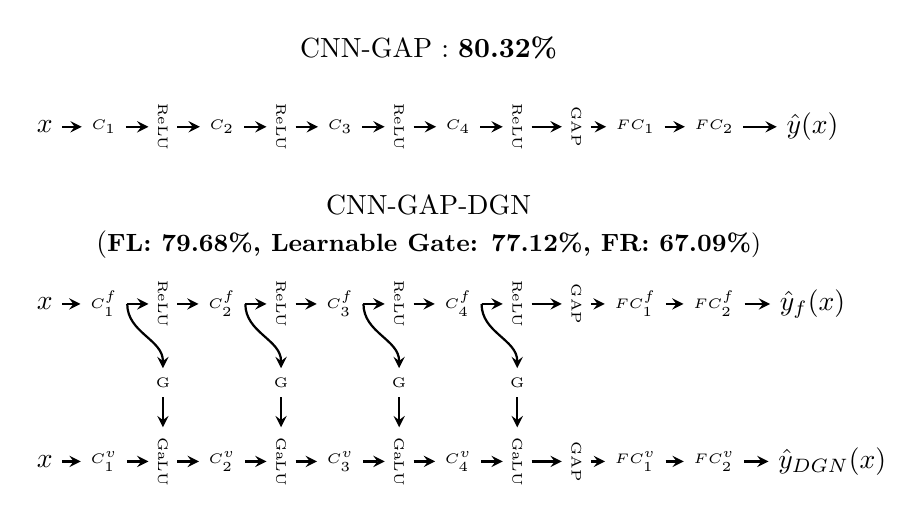
\begin{tikzpicture}
\node []  (dnn-text)at (5.375,2) {CNN-GAP : \textbf{80.32\%}};

\node []  (dnn-output) at (10.25,1) {$\hat{y}(x)$};
\node []  (dnn-fc2) at (9.0,1) {\tiny{$FC_2$}};
\draw [-stealth,thick]   (dnn-fc2.east) -- (dnn-output.west);

\node []  (dnn-fc1) at (8,1) {\tiny{$FC_1$}};
\draw [-stealth,thick]   (dnn-fc1.east) -- (dnn-fc2.west);

\node [rotate=-90]  (dnn-gap) at (7.25,1) {\tiny{GAP}};
\draw [-stealth,thick]   (dnn-gap.north) -- (dnn-fc1.west);

\node [rotate=-90] (dnn-relu-4) at (6.5,1){\tiny{ReLU}};
\node [] (dnn-c4) at (5.75,1){\tiny{$C_4$}};
\draw [-stealth,thick]   (dnn-c4.east) -- (dnn-relu-4.south);
\draw [-stealth,thick]   (dnn-relu-4.north) -- (dnn-gap.south);



\node [rotate=-90] (dnn-relu-3) at (5,1){\tiny{ReLU}};
\node [] (dnn-c3) at (4.25,1){\tiny{$C_3$}};
\draw [-stealth,thick]   (dnn-c3.east) -- (dnn-relu-3.south);
\draw [-stealth,thick]   (dnn-relu-3.north) -- (dnn-c4.west);


\node [rotate=-90] (dnn-relu-2) at (3.5,1){\tiny{ReLU}};
\node [] (dnn-c2) at (2.75,1){\tiny{$C_2$}};
\draw [-stealth,thick]   (dnn-c2.east) -- (dnn-relu-2.south);
\draw [-stealth,thick]   (dnn-relu-2.north) -- (dnn-c3.west);

\node [rotate=-90] (dnn-relu-1) at (2,1){\tiny{ReLU}};
\node [] (dnn-c1) at (1.25,1){\tiny{$C_1$}};
\draw [-stealth,thick]   (dnn-c1.east) -- (dnn-relu-1.south);
\draw [-stealth,thick]   (dnn-relu-1.north) -- (dnn-c2.west);



\node [] (dnn-input) at (0.5,1){$x$};
\draw [-stealth,thick]   (dnn-input.east) -- (dnn-c1.west);


%%%%%%%%%%%%%%%%%%%%%%%%%%%%%%%%%%%%%%%%%%%%%%%%%%%%%%%%%%%%%%%%%
\node []  (fntext)at (5.375,0) {CNN-GAP-DGN};
\node []  (fntext)at (5.375,-.5) {(\small{\textbf{FL: 79.68\%, Learnable Gate: 77.12\%, FR: 67.09\%}})};

%\node []  (output) at (7.5,1.5) {$\hat{y}(x)$};


\node [align=right]  (dgn-f-output) at (10.25,-1.25) {$\hat{y}_{\text{f}}(x)$};
\node []  (dgn-f-fc2) at (9.0,-1.25) {\tiny{$FC^{\text{f}}_2$}};
\draw [-stealth,thick]   (dgn-f-fc2.east) -- (dgn-f-output.west);


\node []  (dgn-f-fc1) at (8,-1.25) {\tiny{$FC^{\text{f}}_1$}};
\draw [-stealth,thick]   (dgn-f-fc1.east) -- (dgn-f-fc2.west);




\node [rotate=-90]  (dgn-f-gap) at (7.25,-1.25) {\tiny{GAP}};
\draw [-stealth,thick]   (dgn-f-gap.north) -- (dgn-f-fc1.west);


\node [rotate=-90] (dgn-relu-4) at (6.5,-1.25){\tiny{ReLU}};
\node [] (dgn-f-c4) at (5.75,-1.25){\tiny{$C^{\text{f}}_4$}};
\draw [-stealth,thick]   (dgn-f-c4.east) -- (dgn-relu-4.south);
\draw [-stealth,thick]   (dgn-relu-4.north) -- (dgn-f-gap.south);


\node [rotate=-90] (dgn-relu-3) at (5,-1.25){\tiny{ReLU}};
\node [] (dgn-f-c3) at (4.25,-1.25){\tiny{$C^{\text{f}}_3$}};
\draw [-stealth,thick]   (dgn-f-c3.east) -- (dgn-relu-3.south);
\draw [-stealth,thick]   (dgn-relu-3.north) -- (dgn-f-c4.west);


\node [rotate=-90] (dgn-relu-2) at (3.5,-1.25){\tiny{ReLU}};
\node [] (dgn-f-c2) at (2.75,-1.25){\tiny{$C^{\text{f}}_2$}};
\draw [-stealth,thick]   (dgn-f-c2.east) -- (dgn-relu-2.south);
\draw [-stealth,thick]   (dgn-relu-2.north) -- (dgn-f-c3.west);


\node [rotate=-90] (dgn-relu-1) at (2,-1.25){\tiny{ReLU}};
\node [] (dgn-f-c1) at (1.25,-1.25){\tiny{$C^{\text{f}}_1$}};
\draw [-stealth,thick]   (dgn-f-c1.east) -- (dgn-relu-1.south);
\draw [-stealth,thick]   (dgn-relu-1.north) -- (dgn-f-c2.west);



\node [] (dgn-f-input) at (0.5,-1.25){$x$};
\draw [-stealth,thick]   (dgn-f-input.east) -- (dgn-f-c1.west);

\node [align=right]  (dgn-output) at (10.5,-3.25) {$\hat{y}_{\text{DGN}}(x)$};

\node [] (dgn-fc2) at (9,-3.25){\tiny{$FC^{\text{v}}_2$}};
\draw [-stealth,thick]   (dgn-fc2.east)--(dgn-output.west);

\node [] (dgn-fc1) at (8,-3.25){\tiny{$FC^{\text{v}}_1$}};
\draw [-stealth,thick]   (dgn-fc1.east)--(dgn-fc2.west);

\node [rotate=-90] (dgn-gap) at (7.25,-3.25){\tiny{GAP}};
\draw [-stealth,thick]   (dgn-gap.north)--(dgn-fc1.west);



\node [rotate=-90] (dgn-galu-4) at (6.5,-3.25){\tiny{GaLU}};
\draw [-stealth,thick]   (dgn-galu-4.north) -- (dgn-gap.south);

\node [] (dgn-v-c4) at (5.75,-3.25){\tiny{$C^{\text{v}}_4$}};
\draw [-stealth,thick]   (dgn-v-c4.east) -- (dgn-galu-4.south);

\node [rotate=-90] (dgn-galu-3) at (5,-3.25){\tiny{GaLU}};
\node [] (dgn-v-c3) at (4.25,-3.25){\tiny{$C^{\text{v}}_3$}};
\draw [-stealth,thick]   (dgn-v-c3.east) -- (dgn-galu-3.south);
\draw [-stealth,thick]   (dgn-galu-3.north) -- (dgn-v-c4.west);



\node [rotate=-90] (dgn-galu-2) at (3.5,-3.25){\tiny{GaLU}};
\node [] (dgn-v-c2) at (2.75,-3.25){\tiny{$C^{\text{v}}_2$}};
\draw [-stealth,thick]   (dgn-v-c2.east) -- (dgn-galu-2.south);
\draw [-stealth,thick]   (dgn-galu-2.north) -- (dgn-v-c3.west);


\node [rotate=-90] (dgn-galu-1) at (2,-3.25){\tiny{GaLU}};
\node [] (dgn-v-c1) at (1.25,-3.25){\tiny{$C^{\text{v}}_1$}};

\draw [-stealth,thick]   (dgn-v-c1.east) -- (dgn-galu-1.south);
\draw [-stealth,thick]   (dgn-galu-1.north) -- (dgn-v-c2.west);




\node [] (dgn-input) at (0.5,-3.25){$x$};
\draw [-stealth,thick]   (dgn-input.east) -- (dgn-v-c1.west);




\node[] (dgn-gating-1) at (2,-2.25){\tiny{G}};
\draw [-stealth,thick]   (dgn-f-c1.east) to[out=-90,in=90] (dgn-gating-1.north);
\draw [-stealth,thick]   (dgn-gating-1.south) -- (dgn-galu-1.west);


\node[] (dgn-gating-2) at (3.5,-2.25){\tiny{G}};
\draw [-stealth,thick]   (dgn-f-c2.east) to[out=-90,in=90] (dgn-gating-2.north);
\draw [-stealth,thick]   (dgn-gating-2.south) -- (dgn-galu-2.west);



\node[] (dgn-gating-3) at (5,-2.25){\tiny{G}};
\draw [-stealth,thick]   (dgn-f-c3.east) to[out=-90,in=90] (dgn-gating-3.north);
\draw [-stealth,thick]   (dgn-gating-3.south) -- (dgn-galu-3.west);


\node[] (dgn-gating-4) at (6.5,-2.25){\tiny{G}};
\draw [-stealth,thick]   (dgn-f-c4.east) to[out=-90,in=90] (dgn-gating-4.north);
\draw [-stealth,thick]   (dgn-gating-4.south) -- (dgn-galu-4.west);

	
\end{tikzpicture}


}
\end{minipage}
\begin{minipage}{0.3\columnwidth}
\resizebox{!}{20cm}{
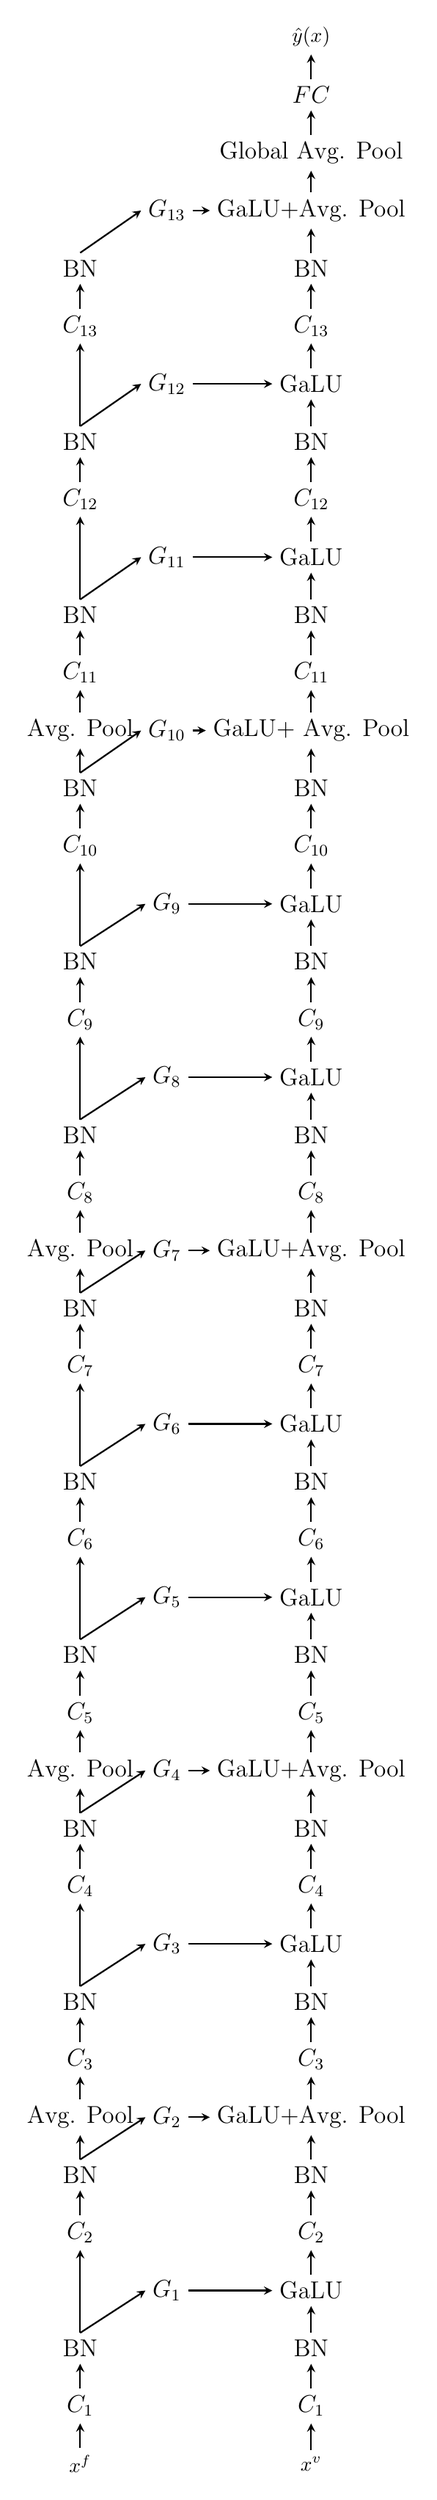
\begin{tikzpicture}


%\node [] (dgn-GaLU-16) at (4,48){\large{GaLU}};
%\draw [-stealth,thick]   (dgn-GaLU-16.north) -- (dgn-c9.south);

%\node [] (dgn-bn-16) at (4,47){\large{BN}};
%\draw [-stealth,thick]   (dgn-bn-16.north) -- (dgn-GaLU-16.south);

%\node [] (dgn-c16) at (4,46){\large{$C_{16}$}};
%\draw [-stealth,thick]   (dgn-c16.north) -- (dgn-bn-16.south);




%\node [] (dgn-GaLU-15) at (4,45){\large{GaLU}};
%\draw [-stealth,thick]   (dgn-GaLU-15.north) -- (dgn-c16.south);

%\node [] (dgn-bn-15) at (4,44){\large{BN}};
%\draw [-stealth,thick]   (dgn-bn-15.north) -- (dgn-GaLU-15.south);

%\node [] (dgn-c15) at (4,43){\large{$C_{15}$}};
%\draw [-stealth,thick]   (dgn-c15.north) -- (dgn-bn-15.south);




\node [] (dgn-GaLU-14) at (4,42){$\hat{y}(x)$};
%\draw [-stealth,thick]   (dgn-GaLU-14.north) -- (dgn-c15.south);

\node [] (dgn-bn-14) at (4,41){\large{$FC$}};
\draw [-stealth,thick]   (dgn-bn-14.north) -- (dgn-GaLU-14.south);

\node [] (dgn-c14) at (4,40){\large{Global Avg. Pool}};
\draw [-stealth,thick]   (dgn-c14.north) -- (dgn-bn-14.south);




\node [] (dgn-GaLU-13) at (4,39){\large{GaLU+Avg. Pool}};
\draw [-stealth,thick]   (dgn-GaLU-13.north) -- (dgn-c14.south);

\node [] (dgn-bn-13) at (4,38){\large{BN}};
\draw [-stealth,thick]   (dgn-bn-13.north) -- (dgn-GaLU-13.south);

\node [] (dgn-c13) at (4,37){\large{$C_{13}$}};
\draw [-stealth,thick]   (dgn-c13.north) -- (dgn-bn-13.south);



\node [] (dgn-GaLU-12) at (4,36){\large{GaLU}};
\draw [-stealth,thick]   (dgn-GaLU-12.north) -- (dgn-c13.south);

\node [] (dgn-bn-12) at (4,35){\large{BN}};
\draw [-stealth,thick]   (dgn-bn-12.north) -- (dgn-GaLU-12.south);

\node [] (dgn-c12) at (4,34){\large{$C_{12}$}};
\draw [-stealth,thick]   (dgn-c12.north) -- (dgn-bn-12.south);



\node [] (dgn-GaLU-11) at (4,33){\large{GaLU}};
\draw [-stealth,thick]   (dgn-GaLU-11.north) -- (dgn-c12.south);

\node [] (dgn-bn-11) at (4,32){\large{BN}};
\draw [-stealth,thick]   (dgn-bn-11.north) -- (dgn-GaLU-11.south);

\node [] (dgn-c11) at (4,31){\large{$C_{11}$}};
\draw [-stealth,thick]   (dgn-c11.north) -- (dgn-bn-11.south);





\node [] (dgn-GaLU-10) at (4,30){\large{GaLU+ Avg. Pool}};
\draw [-stealth,thick]   (dgn-GaLU-10.north) -- (dgn-c11.south);

\node [] (dgn-bn-10) at (4,29){\large{BN}};
\draw [-stealth,thick]   (dgn-bn-10.north) -- (dgn-GaLU-10.south);

\node [] (dgn-c10) at (4,28){\large{$C_{10}$}};
\draw [-stealth,thick]   (dgn-c10.north) -- (dgn-bn-10.south);




\node [] (dgn-GaLU-9) at (4,27){\large{GaLU}};
\draw [-stealth,thick]   (dgn-GaLU-9.north) -- (dgn-c10.south);

\node [] (dgn-bn-9) at (4,26){\large{BN}};
\draw [-stealth,thick]   (dgn-bn-9.north) -- (dgn-GaLU-9.south);

\node [] (dgn-c9) at (4,25){\large{$C_9$}};
\draw [-stealth,thick]   (dgn-c9.north) -- (dgn-bn-9.south);



\node [] (dgn-GaLU-8) at (4,24){\large{GaLU}};
\draw [-stealth,thick]   (dgn-GaLU-8.north) -- (dgn-c9.south);

\node [] (dgn-bn-8) at (4,23){\large{BN}};
\draw [-stealth,thick]   (dgn-bn-8.north) -- (dgn-GaLU-8.south);

\node [] (dgn-c8) at (4,22){\large{$C_8$}};
\draw [-stealth,thick]   (dgn-c8.north) -- (dgn-bn-8.south);




\node [] (dgn-GaLU-7) at (4,21){\large{GaLU+Avg. Pool}};
\draw [-stealth,thick]   (dgn-GaLU-7.north) -- (dgn-c8.south);

\node [] (dgn-bn-7) at (4,20){\large{BN}};
\draw [-stealth,thick]   (dgn-bn-7.north) -- (dgn-GaLU-7.south);

\node [] (dgn-c7) at (4,19){\large{$C_7$}};
\draw [-stealth,thick]   (dgn-c7.north) -- (dgn-bn-7.south);




\node [] (dgn-GaLU-6) at (4,18){\large{GaLU}};
\draw [-stealth,thick]   (dgn-GaLU-6.north) -- (dgn-c7.south);

\node [] (dgn-bn-6) at (4,17){\large{BN}};
\draw [-stealth,thick]   (dgn-bn-6.north) -- (dgn-GaLU-6.south);

\node [] (dgn-c6) at (4,16){\large{$C_6$}};
\draw [-stealth,thick]   (dgn-c6.north) -- (dgn-bn-6.south);




\node [] (dgn-GaLU-5) at (4,15){\large{GaLU}};
\draw [-stealth,thick]   (dgn-GaLU-5.north) -- (dgn-c6.south);

\node [] (dgn-bn-5) at (4,14){\large{BN}};
\draw [-stealth,thick]   (dgn-bn-5.north) -- (dgn-GaLU-5.south);

\node [] (dgn-c5) at (4,13){\large{$C_5$}};
\draw [-stealth,thick]   (dgn-c5.north) -- (dgn-bn-5.south);



\node [] (dgn-GaLU-4) at (4,12){\large{GaLU+Avg. Pool}};
\draw [-stealth,thick]   (dgn-GaLU-4.north) -- (dgn-c5.south);

\node [] (dgn-bn-4) at (4,11){\large{BN}};
\draw [-stealth,thick]   (dgn-bn-4.north) -- (dgn-GaLU-4.south);

\node [] (dgn-c4) at (4,10){\large{$C_4$}};
\draw [-stealth,thick]   (dgn-c4.north) -- (dgn-bn-4.south);



\node [] (dgn-GaLU-3) at (4,9){\large{GaLU}};
\draw [-stealth,thick]   (dgn-GaLU-3.north) -- (dgn-c4.south);

\node [] (dgn-bn-3) at (4,8){\large{BN}};
\draw [-stealth,thick]   (dgn-bn-3.north) -- (dgn-GaLU-3.south);

\node [] (dgn-c3) at (4,7){\large{$C_3$}};
\draw [-stealth,thick]   (dgn-c3.north) -- (dgn-bn-3.south);





\node [] (dgn-GaLU-2) at (4,6){\large{GaLU+Avg. Pool}};
\draw [-stealth,thick]   (dgn-GaLU-2.north) -- (dgn-c3.south);

\node [] (dgn-bn-2) at (4,5){\large{BN}};
\draw [-stealth,thick]   (dgn-bn-2.north) -- (dgn-GaLU-2.south);

\node [] (dgn-c2) at (4,4){\large{$C_2$}};
\draw [-stealth,thick]   (dgn-c2.north) -- (dgn-bn-2.south);




\node [] (dgn-GaLU-1) at (4,3){\large{GaLU}};
\draw [-stealth,thick]   (dgn-GaLU-1.north) -- (dgn-c2.south);

\node [] (dgn-bn-1) at (4,2){\large{BN}};
\draw [-stealth,thick]   (dgn-bn-1.north) -- (dgn-GaLU-1.south);

\node [] (dgn-c1) at (4,1){\large{$C_1$}};
\draw [-stealth,thick]   (dgn-c1.north) -- (dgn-bn-1.south);



\node [] (dgn-input) at (4,0){$x^{\text{v}}$};
\draw [-stealth,thick]   (dgn-input.north) -- (dgn-c1.south);


%%%%%%%%%%%%%%%%%%%%%%%%%%%%%%%%%%%%%%%%%%%%%%%%%%%%%%%%%%%%%%%%%


%\node [] (dnn-relu-16) at (0,48){\large{ReLU}};
%\draw [-stealth,thick]   (dnn-relu-16.north) -- (dnn-c9.south);

%\node [] (dnn-bn-16) at (0,47){\large{BN}};
%\draw [-stealth,thick]   (dnn-bn-16.north) -- (dnn-relu-16.south);

%\node [] (dnn-c16) at (0,46){\large{$C_{16}$}};
%\draw [-stealth,thick]   (dnn-c16.north) -- (dnn-bn-16.south);




%\node [] (dnn-relu-15) at (0,45){\large{ReLU}};
%\draw [-stealth,thick]   (dnn-relu-15.north) -- (dnn-c16.south);

%\node [] (dnn-bn-15) at (0,44){\large{BN}};
%\draw [-stealth,thick]   (dnn-bn-15.north) -- (dnn-relu-15.south);

%\node [] (dnn-c15) at (0,43){\large{$C_{15}$}};
%\draw [-stealth,thick]   (dnn-c15.north) -- (dnn-bn-15.south);




%\node [] (dnn-relu-14) at (0,42){\large{Softmax}};
%\draw [-stealth,thick]   (dnn-relu-14.north) -- (dnn-c15.south);

%\node [] (dnn-bn-14) at (0,41){\large{Fully Connected}};
%\draw [-stealth,thick]   (dnn-bn-14.north) -- (dnn-relu-14.south);

%\node [] (dnn-c14) at (0,40){\large{Global Avg. Pool}};
%\draw [-stealth,thick]   (dnn-c14.north) -- (dnn-bn-14.south);




%\node [] (dnn-relu-13) at (0,39){\large{Avg. Pool}};
%\draw [-stealth,thick]   (dnn-relu-13.north) -- (dnn-c14.south);

\node [] (dnn-bn-13) at (0,38){\large{BN}};
%\draw [-stealth,thick]   (dnn-bn-13.north) -- (dnn-relu-13.south);

\node [] (dnn-gate-13) at (1.5,39){\large{$G_{13}$}};
\draw [-stealth,thick]   (dnn-bn-13.north) -- (dnn-gate-13.west);
\draw [-stealth,thick]   (dnn-gate-13.east) -- (dgn-GaLU-13.west);

\node [] (dnn-c13) at (0,37){\large{$C_{13}$}};
\draw [-stealth,thick]   (dnn-c13.north) -- (dnn-bn-13.south);



%\node [] (dnn-relu-12) at (0,36){\large{ReLU}};
%\draw [-stealth,thick]   (dnn-relu-12.north) -- (dnn-c13.south);

\node [] (dnn-bn-12) at (0,35){\large{BN}};
\draw [-stealth,thick]   (dnn-bn-12.north) -- (dnn-c13.south);

\node [] (dnn-gate-12) at (1.5,36){\large{$G_{12}$}};
\draw [-stealth,thick]   (dnn-bn-12.north) -- (dnn-gate-12.west);
\draw [-stealth,thick]   (dnn-gate-12.east) -- (dgn-GaLU-12.west);

\node [] (dnn-c12) at (0,34){\large{$C_{12}$}};
\draw [-stealth,thick]   (dnn-c12.north) -- (dnn-bn-12.south);



%\node [] (dnn-relu-11) at (0,33){\large{ReLU}};
%\draw [-stealth,thick]   (dnn-relu-11.north) -- (dnn-c12.south);

\node [] (dnn-bn-11) at (0,32){\large{BN}};
\draw [-stealth,thick]   (dnn-bn-11.north) -- (dnn-c12.south);

\node [] (dnn-gate-11) at (1.5,33){\large{$G_{11}$}};
\draw [-stealth,thick]   (dnn-bn-11.north) -- (dnn-gate-11.west);
\draw [-stealth,thick]   (dnn-gate-11.east) -- (dgn-GaLU-11.west);


\node [] (dnn-c11) at (0,31){\large{$C_{11}$}};
\draw [-stealth,thick]   (dnn-c11.north) -- (dnn-bn-11.south);





\node [] (dnn-relu-10) at (0,30){\large{Avg. Pool}};
\draw [-stealth,thick]   (dnn-relu-10.north) -- (dnn-c11.south);

\node [] (dnn-bn-10) at (0,29){\large{BN}};
\draw [-stealth,thick]   (dnn-bn-10.north) -- (dnn-relu-10.south);

\node [] (dnn-gate-10) at (1.5,30){\large{$G_{10}$}};
\draw [-stealth,thick]   (dnn-bn-10.north) -- (dnn-gate-10.west);
\draw [-stealth,thick]   (dnn-gate-10.east) -- (dgn-GaLU-10.west);


\node [] (dnn-c10) at (0,28){\large{$C_{10}$}};
\draw [-stealth,thick]   (dnn-c10.north) -- (dnn-bn-10.south);




%\node [] (dnn-relu-9) at (0,27){\large{ReLU}};
%\draw [-stealth,thick]   (dnn-relu-9.north) -- (dnn-c10.south);

\node [] (dnn-bn-9) at (0,26){\large{BN}};
\draw [-stealth,thick]   (dnn-bn-9.north) -- (dnn-c10.south);

\node [] (dnn-gate-9) at (1.5,27){\large{$G_{9}$}};
\draw [-stealth,thick]   (dnn-bn-9.north) -- (dnn-gate-9.west);
\draw [-stealth,thick]   (dnn-gate-9.east) -- (dgn-GaLU-9.west);

\node [] (dnn-c9) at (0,25){\large{$C_9$}};
\draw [-stealth,thick]   (dnn-c9.north) -- (dnn-bn-9.south);



%\node [] (dnn-relu-8) at (0,24){\large{ReLU}};
%\draw [-stealth,thick]   (dnn-relu-8.north) -- (dnn-c9.south);

\node [] (dnn-bn-8) at (0,23){\large{BN}};
\draw [-stealth,thick]   (dnn-bn-8.north) -- (dnn-c9.south);

\node [] (dnn-gate-8) at (1.5,24){\large{$G_{8}$}};
\draw [-stealth,thick]   (dnn-bn-8.north) -- (dnn-gate-8.west);
\draw [-stealth,thick]   (dnn-gate-8.east) -- (dgn-GaLU-8.west);


\node [] (dnn-c8) at (0,22){\large{$C_8$}};
\draw [-stealth,thick]   (dnn-c8.north) -- (dnn-bn-8.south);




\node [] (dnn-relu-7) at (0,21){\large{Avg. Pool}};
\draw [-stealth,thick]   (dnn-relu-7.north) -- (dnn-c8.south);

\node [] (dnn-bn-7) at (0,20){\large{BN}};
\draw [-stealth,thick]   (dnn-bn-7.north) -- (dnn-relu-7.south);

\node [] (dnn-gate-7) at (1.5,21){\large{$G_{7}$}};
\draw [-stealth,thick]   (dnn-bn-7.north) -- (dnn-gate-7.west);
\draw [-stealth,thick]   (dnn-gate-7.east) -- (dgn-GaLU-7.west);


\node [] (dnn-c7) at (0,19){\large{$C_7$}};
\draw [-stealth,thick]   (dnn-c7.north) -- (dnn-bn-7.south);




%\node [] (dnn-relu-6) at (0,18){\large{ReLU}};
%\draw [-stealth,thick]   (dnn-relu-6.north) -- (dnn-c7.south);

\node [] (dnn-bn-6) at (0,17){\large{BN}};
\draw [-stealth,thick]   (dnn-bn-6.north) -- (dnn-c7.south);

\node [] (dnn-gate-6) at (1.5,18){\large{$G_{6}$}};
\draw [-stealth,thick]   (dnn-bn-6.north) -- (dnn-gate-6.west);
\draw [-stealth,thick]   (dnn-gate-6.east) -- (dgn-GaLU-6.west);



\node [] (dnn-c6) at (0,16){\large{$C_6$}};
\draw [-stealth,thick]   (dnn-c6.north) -- (dnn-bn-6.south);




%\node [] (dnn-relu-5) at (0,15){\large{ReLU}};
%\draw [-stealth,thick]   (dnn-relu-5.north) -- (dnn-c6.south);

\node [] (dnn-bn-5) at (0,14){\large{BN}};
\draw [-stealth,thick]   (dnn-bn-5.north) -- (dnn-c6.south);

\node [] (dnn-gate-5) at (1.5,15){\large{$G_{5}$}};
\draw [-stealth,thick]   (dnn-bn-5.north) -- (dnn-gate-5.west);
\draw [-stealth,thick]   (dnn-gate-5.east) -- (dgn-GaLU-5.west);


\node [] (dnn-c5) at (0,13){\large{$C_5$}};
\draw [-stealth,thick]   (dnn-c5.north) -- (dnn-bn-5.south);



\node [] (dnn-relu-4) at (0,12){\large{Avg. Pool}};
\draw [-stealth,thick]   (dnn-relu-4.north) -- (dnn-c5.south);

\node [] (dnn-bn-4) at (0,11){\large{BN}};
\draw [-stealth,thick]   (dnn-bn-4.north) -- (dnn-relu-4.south);

\node [] (dnn-gate-4) at (1.5,12){\large{$G_{4}$}};
\draw [-stealth,thick]   (dnn-bn-4.north) -- (dnn-gate-4.west);
\draw [-stealth,thick]   (dnn-gate-4.east) -- (dgn-GaLU-4.west);

\node [] (dnn-c4) at (0,10){\large{$C_4$}};
\draw [-stealth,thick]   (dnn-c4.north) -- (dnn-bn-4.south);



%\node [] (dnn-relu-3) at (0,9){\large{ReLU}};
%\draw [-stealth,thick]   (dnn-relu-3.north) -- (dnn-c4.south);

\node [] (dnn-bn-3) at (0,8){\large{BN}};
\draw [-stealth,thick]   (dnn-bn-3.north) -- (dnn-c4.south);

\node [] (dnn-gate-3) at (1.5,9){\large{$G_{3}$}};
\draw [-stealth,thick]   (dnn-bn-3.north) -- (dnn-gate-3.west);
\draw [-stealth,thick]   (dnn-gate-3.east) -- (dgn-GaLU-3.west);

\node [] (dnn-c3) at (0,7){\large{$C_3$}};
\draw [-stealth,thick]   (dnn-c3.north) -- (dnn-bn-3.south);





\node [] (dnn-relu-2) at (0,6){\large{Avg. Pool}};
\draw [-stealth,thick]   (dnn-relu-2.north) -- (dnn-c3.south);

\node [] (dnn-bn-2) at (0,5){\large{BN}};
\draw [-stealth,thick]   (dnn-bn-2.north) -- (dnn-relu-2.south);

\node [] (dnn-gate-2) at (1.5,6){\large{$G_{2}$}};
\draw [-stealth,thick]   (dnn-bn-2.north) -- (dnn-gate-2.west);
\draw [-stealth,thick]   (dnn-gate-2.east) -- (dgn-GaLU-2.west);



\node [] (dnn-c2) at (0,4){\large{$C_2$}};
\draw [-stealth,thick]   (dnn-c2.north) -- (dnn-bn-2.south);





%\draw [-stealth,thick]   (dnn-relu-1.north) -- (dnn-c2.south);

\node [] (dnn-bn-1) at (0,2){\large{BN}};
\draw [-stealth,thick]   (dnn-bn-1.north) -- (dnn-c2.south);

\node [] (dnn-gate-1) at (1.5,3){\large{$G_{1}$}};
\draw [-stealth,thick]   (dnn-bn-1.north) -- (dnn-gate-1.west);
\draw [-stealth,thick]   (dnn-gate-1.east) -- (dgn-GaLU-1.west);


\node [] (dnn-c1) at (0,1){\large{$C_1$}};
\draw [-stealth,thick]   (dnn-c1.north) -- (dnn-bn-1.south);



\node [] (dnn-input) at (0,0){$x^{\text{f}}$};
\draw [-stealth,thick]   (dnn-input.north) -- (dnn-c1.south);

%%%%%%%%%%%%%%%%%%%%%%%%%%%%%%%%%%%%%%%%%%%%%%%%%%%



	
\end{tikzpicture}


}
\end{minipage}
\begin{minipage}{0.3\columnwidth}
\resizebox{!}{20cm}{
\begin{tikzpicture}




%\node [] (dgn-GaLU-16) at (6,48){\large{GaLU}};
%\draw [-stealth,thick]   (dgn-GaLU-16.north) -- (dgn-c9.south);

%\node [] (dgn-bn-16) at (6,47){\large{BN}};
%\draw [-stealth,thick]   (dgn-bn-16.north) -- (dgn-GaLU-16.south);

%\node [] (dgn-c16) at (6,46){\large{$C_{16}$}};
%\draw [-stealth,thick]   (dgn-c16.north) -- (dgn-bn-16.south);




%\node [] (dgn-GaLU-15) at (6,45){\large{GaLU}};
%\draw [-stealth,thick]   (dgn-GaLU-15.north) -- (dgn-c16.south);

%\node [] (dgn-bn-15) at (6,44){\large{BN}};
%\draw [-stealth,thick]   (dgn-bn-15.north) -- (dgn-GaLU-15.south);

%\node [] (dgn-c15) at (6,43){\large{$C_{15}$}};
%\draw [-stealth,thick]   (dgn-c15.north) -- (dgn-bn-15.south);




\node [] (dgn-GaLU-14) at (6,42){$\hat{y}(x)$};
%\draw [-stealth,thick]   (dgn-GaLU-14.north) -- (dgn-c15.south);

\node [] (dgn-bn-14) at (6,41){\large{$FC$}};
\draw [-stealth,thick]   (dgn-bn-14.north) -- (dgn-GaLU-14.south);

\node [] (dgn-c14) at (6,40){\large{Global Avg. Pool}};
\draw [-stealth,thick]   (dgn-c14.north) -- (dgn-bn-14.south);




\node [] (dgn-GaLU-13) at (6,39){\large{GaLU+Avg. Pool}};
\draw [-stealth,thick]   (dgn-GaLU-13.north) -- (dgn-c14.south);

\node [] (dgn-bn-13) at (6,38){\large{BN}};
\draw [-stealth,thick]   (dgn-bn-13.north) -- (dgn-GaLU-13.south);

\node [] (dgn-c13) at (6,37){\large{$C_{13}$}};
\draw [-stealth,thick]   (dgn-c13.north) -- (dgn-bn-13.south);



\node [] (dgn-GaLU-12) at (6,36){\large{GaLU}};
\draw [-stealth,thick]   (dgn-GaLU-12.north) -- (dgn-c13.south);

\node [] (dgn-bn-12) at (6,35){\large{BN}};
\draw [-stealth,thick]   (dgn-bn-12.north) -- (dgn-GaLU-12.south);

\node [] (dgn-c12) at (6,34){\large{$C_{12}$}};
\draw [-stealth,thick]   (dgn-c12.north) -- (dgn-bn-12.south);



\node [] (dgn-GaLU-11) at (6,33){\large{GaLU}};
\draw [-stealth,thick]   (dgn-GaLU-11.north) -- (dgn-c12.south);

\node [] (dgn-bn-11) at (6,32){\large{BN}};
\draw [-stealth,thick]   (dgn-bn-11.north) -- (dgn-GaLU-11.south);

\node [] (dgn-c11) at (6,31){\large{$C_{11}$}};
\draw [-stealth,thick]   (dgn-c11.north) -- (dgn-bn-11.south);





\node [] (dgn-GaLU-10) at (6,30){\large{GaLU+ Avg. Pool}};
\draw [-stealth,thick]   (dgn-GaLU-10.north) -- (dgn-c11.south);

\node [] (dgn-bn-10) at (6,29){\large{BN}};
\draw [-stealth,thick]   (dgn-bn-10.north) -- (dgn-GaLU-10.south);

\node [] (dgn-c10) at (6,28){\large{$C_{10}$}};
\draw [-stealth,thick]   (dgn-c10.north) -- (dgn-bn-10.south);




\node [] (dgn-GaLU-9) at (6,27){\large{GaLU}};
\draw [-stealth,thick]   (dgn-GaLU-9.north) -- (dgn-c10.south);

\node [] (dgn-bn-9) at (6,26){\large{BN}};
\draw [-stealth,thick]   (dgn-bn-9.north) -- (dgn-GaLU-9.south);

\node [] (dgn-c9) at (6,25){\large{$C_9$}};
\draw [-stealth,thick]   (dgn-c9.north) -- (dgn-bn-9.south);



\node [] (dgn-GaLU-8) at (6,24){\large{GaLU}};
\draw [-stealth,thick]   (dgn-GaLU-8.north) -- (dgn-c9.south);

\node [] (dgn-bn-8) at (6,23){\large{BN}};
\draw [-stealth,thick]   (dgn-bn-8.north) -- (dgn-GaLU-8.south);

\node [] (dgn-c8) at (6,22){\large{$C_8$}};
\draw [-stealth,thick]   (dgn-c8.north) -- (dgn-bn-8.south);




\node [] (dgn-GaLU-7) at (6,21){\large{GaLU+Avg. Pool}};
\draw [-stealth,thick]   (dgn-GaLU-7.north) -- (dgn-c8.south);

\node [] (dgn-bn-7) at (6,20){\large{BN}};
\draw [-stealth,thick]   (dgn-bn-7.north) -- (dgn-GaLU-7.south);

\node [] (dgn-c7) at (6,19){\large{$C_7$}};
\draw [-stealth,thick]   (dgn-c7.north) -- (dgn-bn-7.south);




\node [] (dgn-GaLU-6) at (6,18){\large{GaLU}};
\draw [-stealth,thick]   (dgn-GaLU-6.north) -- (dgn-c7.south);

\node [] (dgn-bn-6) at (6,17){\large{BN}};
\draw [-stealth,thick]   (dgn-bn-6.north) -- (dgn-GaLU-6.south);

\node [] (dgn-c6) at (6,16){\large{$C_6$}};
\draw [-stealth,thick]   (dgn-c6.north) -- (dgn-bn-6.south);




\node [] (dgn-GaLU-5) at (6,15){\large{GaLU}};
\draw [-stealth,thick]   (dgn-GaLU-5.north) -- (dgn-c6.south);

\node [] (dgn-bn-5) at (6,14){\large{BN}};
\draw [-stealth,thick]   (dgn-bn-5.north) -- (dgn-GaLU-5.south);

\node [] (dgn-c5) at (6,13){\large{$C_5$}};
\draw [-stealth,thick]   (dgn-c5.north) -- (dgn-bn-5.south);



\node [] (dgn-GaLU-4) at (6,12){\large{GaLU+Avg. Pool}};
\draw [-stealth,thick]   (dgn-GaLU-4.north) -- (dgn-c5.south);

\node [] (dgn-bn-4) at (6,11){\large{BN}};
\draw [-stealth,thick]   (dgn-bn-4.north) -- (dgn-GaLU-4.south);

\node [] (dgn-c4) at (6,10){\large{$C_4$}};
\draw [-stealth,thick]   (dgn-c4.north) -- (dgn-bn-4.south);



\node [] (dgn-GaLU-3) at (6,9){\large{GaLU}};
\draw [-stealth,thick]   (dgn-GaLU-3.north) -- (dgn-c4.south);

\node [] (dgn-bn-3) at (6,8){\large{BN}};
\draw [-stealth,thick]   (dgn-bn-3.north) -- (dgn-GaLU-3.south);

\node [] (dgn-c3) at (6,7){\large{$C_3$}};
\draw [-stealth,thick]   (dgn-c3.north) -- (dgn-bn-3.south);





\node [] (dgn-GaLU-2) at (6,6){\large{GaLU+Avg. Pool}};
\draw [-stealth,thick]   (dgn-GaLU-2.north) -- (dgn-c3.south);

\node [] (dgn-bn-2) at (6,5){\large{BN}};
\draw [-stealth,thick]   (dgn-bn-2.north) -- (dgn-GaLU-2.south);

\node [] (dgn-c2) at (6,4){\large{$C_2$}};
\draw [-stealth,thick]   (dgn-c2.north) -- (dgn-bn-2.south);




\node [] (dgn-GaLU-1) at (6,3){\large{GaLU}};
\draw [-stealth,thick]   (dgn-GaLU-1.north) -- (dgn-c2.south);

\node [] (dgn-bn-1) at (6,2){\large{BN}};
\draw [-stealth,thick]   (dgn-bn-1.north) -- (dgn-GaLU-1.south);

\node [] (dgn-c1) at (6,1){\large{$C_1$}};
\draw [-stealth,thick]   (dgn-c1.north) -- (dgn-bn-1.south);



\node [] (dgn-input) at (6,0){$\mathbf{1}$};
\draw [-stealth,thick]   (dgn-input.north) -- (dgn-c1.south);


%%%%%%%%%%%%%%%%%%%%%%%%%%%%%%%%%%%%%%%%%%%%%%%%%%%%%%%%%%%%%%%%%


%\node [] (dnnsig-relu-16) at (2,48){\large{ReLU}};
%\draw [-stealth,thick]   (dnnsig-relu-16.north) -- (dnnsig-c9.south);

%\node [] (dnnsig-bn-16) at (2,47){\large{BN}};
%\draw [-stealth,thick]   (dnnsig-bn-16.north) -- (dnnsig-relu-16.south);

%\node [] (dnnsig-c16) at (2,46){\large{$C_{16}$}};
%\draw [-stealth,thick]   (dnnsig-c16.north) -- (dnnsig-bn-16.south);




%\node [] (dnnsig-relu-15) at (2,45){\large{ReLU}};
%\draw [-stealth,thick]   (dnnsig-relu-15.north) -- (dnnsig-c16.south);

%\node [] (dnnsig-bn-15) at (2,44){\large{BN}};
%\draw [-stealth,thick]   (dnnsig-bn-15.north) -- (dnnsig-relu-15.south);

%\node [] (dnnsig-c15) at (2,43){\large{$C_{15}$}};
%\draw [-stealth,thick]   (dnnsig-c15.north) -- (dnnsig-bn-15.south);




%\node [] (dnnsig-relu-14) at (2,42){\large{Softmax}};
%\draw [-stealth,thick]   (dnnsig-relu-14.north) -- (dnnsig-c15.south);

%\node [] (dnnsig-bn-14) at (2,41){\large{Fully Connected}};
%\draw [-stealth,thick]   (dnnsig-bn-14.north) -- (dnnsig-relu-14.south);

%\node [] (dnnsig-c14) at (2,40){\large{Global Avg. Pool}};
%\draw [-stealth,thick]   (dnnsig-c14.north) -- (dnnsig-bn-14.south);




%\node [] (dnnsig-relu-13) at (2,39){\large{Avg. Pool}};
%\draw [-stealth,thick]   (dnnsig-relu-13.north) -- (dnnsig-c14.south);

\node [] (dnnsig-bn-13) at (2,38){\large{BN}};
%\draw [-stealth,thick]   (dnnsig-bn-13.north) -- (dnnsig-relu-13.south);

\node [] (dnnsig-gate-13) at (3.5,39){\large{G}};
\draw [-stealth,thick]   (dnnsig-bn-13.north) -- (dnnsig-gate-13.west);
\draw [-stealth,thick]   (dnnsig-gate-13.east) -- (dgn-GaLU-13.west);

\node [] (dnnsig-c13) at (2,37){\large{$C_{13}$}};
\draw [-stealth,thick]   (dnnsig-c13.north) -- (dnnsig-bn-13.south);



%\node [] (dnnsig-relu-12) at (2,36){\large{ReLU}};
%\draw [-stealth,thick]   (dnnsig-relu-12.north) -- (dnnsig-c13.south);

\node [] (dnnsig-bn-12) at (2,35){\large{BN}};
%\draw [-stealth,thick]   (dnnsig-bn-12.north) -- (dnnsig-c13.south);

\node [] (dnnsig-gate-12) at (3.5,36){\large{G}};
\draw [-stealth,thick]   (dnnsig-bn-12.north) -- (dnnsig-gate-12.west);
\draw [-stealth,thick]   (dnnsig-gate-12.east) -- (dgn-GaLU-12.west);

\node [] (dnnsig-c12) at (2,34){\large{$C_{12}$}};
\draw [-stealth,thick]   (dnnsig-c12.north) -- (dnnsig-bn-12.south);



%\node [] (dnnsig-relu-11) at (2,33){\large{ReLU}};
%\draw [-stealth,thick]   (dnnsig-relu-11.north) -- (dnnsig-c12.south);

\node [] (dnnsig-bn-11) at (2,32){\large{BN}};
%\draw [-stealth,thick]   (dnnsig-bn-11.north) -- (dnnsig-c12.south);

\node [] (dnnsig-gate-11) at (3.5,33){\large{G}};
\draw [-stealth,thick]   (dnnsig-bn-11.north) -- (dnnsig-gate-11.west);
\draw [-stealth,thick]   (dnnsig-gate-11.east) -- (dgn-GaLU-11.west);


\node [] (dnnsig-c11) at (2,31){\large{$C_{11}$}};
\draw [-stealth,thick]   (dnnsig-c11.north) -- (dnnsig-bn-11.south);





%\node [] (dnnsig-relu-10) at (2,30){\large{Avg. Pool}};
%\draw [-stealth,thick]   (dnnsig-relu-10.north) -- (dnnsig-c11.south);

\node [] (dnnsig-bn-10) at (2,29){\large{BN}};
%\draw [-stealth,thick]   (dnnsig-bn-10.north) -- (dnnsig-relu-10.south);

\node [] (dnnsig-gate-10) at (3.5,30){\large{G}};
\draw [-stealth,thick]   (dnnsig-bn-10.north) -- (dnnsig-gate-10.west);
\draw [-stealth,thick]   (dnnsig-gate-10.east) -- (dgn-GaLU-10.west);


\node [] (dnnsig-c10) at (2,28){\large{$C_{10}$}};
\draw [-stealth,thick]   (dnnsig-c10.north) -- (dnnsig-bn-10.south);




%\node [] (dnnsig-relu-9) at (2,27){\large{ReLU}};
%\draw [-stealth,thick]   (dnnsig-relu-9.north) -- (dnnsig-c10.south);

\node [] (dnnsig-bn-9) at (2,26){\large{BN}};
%\draw [-stealth,thick]   (dnnsig-bn-9.north) -- (dnnsig-c10.south);

\node [] (dnnsig-gate-9) at (3.5,27){\large{G}};
\draw [-stealth,thick]   (dnnsig-bn-9.north) -- (dnnsig-gate-9.west);
\draw [-stealth,thick]   (dnnsig-gate-9.east) -- (dgn-GaLU-9.west);

\node [] (dnnsig-c9) at (2,25){\large{$C_9$}};
\draw [-stealth,thick]   (dnnsig-c9.north) -- (dnnsig-bn-9.south);



%\node [] (dnnsig-relu-8) at (2,24){\large{ReLU}};
%\draw [-stealth,thick]   (dnnsig-relu-8.north) -- (dnnsig-c9.south);

\node [] (dnnsig-bn-8) at (2,23){\large{BN}};
%\draw [-stealth,thick]   (dnnsig-bn-8.north) -- (dnnsig-c9.south);

\node [] (dnnsig-gate-8) at (3.5,24){\large{G}};
\draw [-stealth,thick]   (dnnsig-bn-8.north) -- (dnnsig-gate-8.west);
\draw [-stealth,thick]   (dnnsig-gate-8.east) -- (dgn-GaLU-8.west);


\node [] (dnnsig-c8) at (2,22){\large{$C_8$}};
\draw [-stealth,thick]   (dnnsig-c8.north) -- (dnnsig-bn-8.south);




%\node [] (dnnsig-relu-7) at (2,21){\large{Avg. Pool}};
%\draw [-stealth,thick]   (dnnsig-relu-7.north) -- (dnnsig-c8.south);

\node [] (dnnsig-bn-7) at (2,20){\large{BN}};
%\draw [-stealth,thick]   (dnnsig-bn-7.north) -- (dnnsig-relu-7.south);

\node [] (dnnsig-gate-7) at (3.5,21){\large{G}};
\draw [-stealth,thick]   (dnnsig-bn-7.north) -- (dnnsig-gate-7.west);
\draw [-stealth,thick]   (dnnsig-gate-7.east) -- (dgn-GaLU-7.west);


\node [] (dnnsig-c7) at (2,19){\large{$C_7$}};
\draw [-stealth,thick]   (dnnsig-c7.north) -- (dnnsig-bn-7.south);




%\node [] (dnnsig-relu-6) at (2,18){\large{ReLU}};
%\draw [-stealth,thick]   (dnnsig-relu-6.north) -- (dnnsig-c7.south);

\node [] (dnnsig-bn-6) at (2,17){\large{BN}};
%\draw [-stealth,thick]   (dnnsig-bn-6.north) -- (dnnsig-c7.south);

\node [] (dnnsig-gate-6) at (3.5,18){\large{G}};
\draw [-stealth,thick]   (dnnsig-bn-6.north) -- (dnnsig-gate-6.west);
\draw [-stealth,thick]   (dnnsig-gate-6.east) -- (dgn-GaLU-6.west);



\node [] (dnnsig-c6) at (2,16){\large{$C_6$}};
\draw [-stealth,thick]   (dnnsig-c6.north) -- (dnnsig-bn-6.south);




%\node [] (dnnsig-relu-5) at (2,15){\large{ReLU}};
%\draw [-stealth,thick]   (dnnsig-relu-5.north) -- (dnnsig-c6.south);

\node [] (dnnsig-bn-5) at (2,14){\large{BN}};
%\draw [-stealth,thick]   (dnnsig-bn-5.north) -- (dnnsig-c6.south);

\node [] (dnnsig-gate-5) at (3.5,15){\large{G}};
\draw [-stealth,thick]   (dnnsig-bn-5.north) -- (dnnsig-gate-5.west);
\draw [-stealth,thick]   (dnnsig-gate-5.east) -- (dgn-GaLU-5.west);


\node [] (dnnsig-c5) at (2,13){\large{$C_5$}};
\draw [-stealth,thick]   (dnnsig-c5.north) -- (dnnsig-bn-5.south);



%\node [] (dnnsig-relu-4) at (2,12){\large{Avg. Pool}};
%\draw [-stealth,thick]   (dnnsig-relu-4.north) -- (dnnsig-c5.south);

\node [] (dnnsig-bn-4) at (2,11){\large{BN}};
%\draw [-stealth,thick]   (dnnsig-bn-4.north) -- (dnnsig-relu-4.south);

\node [] (dnnsig-gate-4) at (3.5,12){\large{G}};
\draw [-stealth,thick]   (dnnsig-bn-4.north) -- (dnnsig-gate-4.west);
\draw [-stealth,thick]   (dnnsig-gate-4.east) -- (dgn-GaLU-4.west);

\node [] (dnnsig-c4) at (2,10){\large{$C_4$}};
\draw [-stealth,thick]   (dnnsig-c4.north) -- (dnnsig-bn-4.south);



%\node [] (dnnsig-relu-3) at (2,9){\large{ReLU}};
%\draw [-stealth,thick]   (dnnsig-relu-3.north) -- (dnnsig-c4.south);

\node [] (dnnsig-bn-3) at (2,8){\large{BN}};
%\draw [-stealth,thick]   (dnnsig-bn-3.north) -- (dnnsig-c4.south);

\node [] (dnnsig-gate-3) at (3.5,9){\large{G}};
\draw [-stealth,thick]   (dnnsig-bn-3.north) -- (dnnsig-gate-3.west);
\draw [-stealth,thick]   (dnnsig-gate-3.east) -- (dgn-GaLU-3.west);

\node [] (dnnsig-c3) at (2,7){\large{$C_3$}};
\draw [-stealth,thick]   (dnnsig-c3.north) -- (dnnsig-bn-3.south);





%\node [] (dnnsig-relu-2) at (2,6){\large{Avg. Pool}};
%\draw [-stealth,thick]   (dnnsig-relu-2.north) -- (dnnsig-c3.south);

\node [] (dnnsig-bn-2) at (2,5){\large{BN}};
%\draw [-stealth,thick]   (dnnsig-bn-2.north) -- (dnnsig-relu-2.south);

\node [] (dnnsig-gate-2) at (3.5,6){\large{G}};
\draw [-stealth,thick]   (dnnsig-bn-2.north) -- (dnnsig-gate-2.west);
\draw [-stealth,thick]   (dnnsig-gate-2.east) -- (dgn-GaLU-2.west);



\node [] (dnnsig-c2) at (2,4){\large{$C_2$}};
\draw [-stealth,thick]   (dnnsig-c2.north) -- (dnnsig-bn-2.south);





%\draw [-stealth,thick]   (dnnsig-relu-1.north) -- (dnnsig-c2.south);

\node [] (dnnsig-bn-1) at (2,2){\large{BN}};
%\draw [-stealth,thick]   (dnnsig-bn-1.north) -- (dnnsig-c2.south);

\node [] (dnnsig-gate-1) at (3.5,3){\large{G}};
\draw [-stealth,thick]   (dnnsig-bn-1.north) -- (dnnsig-gate-1.west);
\draw [-stealth,thick]   (dnnsig-gate-1.east) -- (dgn-GaLU-1.west);


\node [] (dnnsig-c1) at (2,1){\large{$C_1$}};
\draw [-stealth,thick]   (dnnsig-c1.north) -- (dnnsig-bn-1.south);



%\node [] (dnnsig-input) at (2,0){$x$};


\draw [-stealth,thick]   (dnn-c1.center) -- (dnnsig-c1.west);
\draw [-stealth,thick]   (dnn-c2.center) -- (dnnsig-c2.west);
\draw [-stealth,thick]   (dnn-c3.center) -- (dnnsig-c3.west);
\draw [-stealth,thick]   (dnn-c4.center) -- (dnnsig-c4.west);
\draw [-stealth,thick]   (dnn-c5.center) -- (dnnsig-c5.west);
\draw [-stealth,thick]   (dnn-c6.center) -- (dnnsig-c6.west);
\draw [-stealth,thick]   (dnn-c7.center) -- (dnnsig-c7.west);
\draw [-stealth,thick]   (dnn-c8.center) -- (dnnsig-c8.west);
\draw [-stealth,thick]   (dnn-c9.center) -- (dnnsig-c9.west);
\draw [-stealth,thick]   (dnn-c10.center) -- (dnnsig-c10.west);
\draw [-stealth,thick]   (dnn-c11.center) -- (dnnsig-c11.west);
\draw [-stealth,thick]   (dnn-c12.center) -- (dnnsig-c12.west);
\draw [-stealth,thick]   (dnn-c13.center) -- (dnnsig-c13.west);





%\draw [-stealth,thick]   (dnnsig-input.north) -- (dnnsig-c1.south);

%%%%%%%%%%%%%%%%%%%%%%%%%%%%%%%%%%%%%%%%%%%%%%%%%%%

%%%%%%%%%%%%%%%%%%%%%%%%%%%%%%%%%%%%%%%%%%%%%%%%%%%%%%%%%%%%%%%%%



%\node [] (dnn-relu-16) at (0,48){\large{ReLU}};
%\draw [-stealth,thick]   (dnn-relu-16.north) -- (dnn-c9.south);

%\node [] (dnn-bn-16) at (0,47){\large{BN}};
%\draw [-stealth,thick]   (dnn-bn-16.north) -- (dnn-relu-16.south);

%\node [] (dnn-c16) at (0,46){\large{$C_{16}$}};
%\draw [-stealth,thick]   (dnn-c16.north) -- (dnn-bn-16.south);




%\node [] (dnn-relu-15) at (0,45){\large{ReLU}};
%\draw [-stealth,thick]   (dnn-relu-15.north) -- (dnn-c16.south);

%\node [] (dnn-bn-15) at (0,44){\large{BN}};
%\draw [-stealth,thick]   (dnn-bn-15.north) -- (dnn-relu-15.south);

%\node [] (dnn-c15) at (0,43){\large{$C_{15}$}};
%\draw [-stealth,thick]   (dnn-c15.north) -- (dnn-bn-15.south);




%\node [] (dnn-relu-14) at (0,42){\large{Softmax}};
%\draw [-stealth,thick]   (dnn-relu-14.north) -- (dnn-c15.south);

%\node [] (dnn-bn-14) at (0,41){\large{Fully Connected}};
%\draw [-stealth,thick]   (dnn-bn-14.north) -- (dnn-relu-14.south);

%\node [] (dnn-c14) at (0,40){\large{Global Avg. Pool}};
%\draw [-stealth,thick]   (dnn-c14.north) -- (dnn-bn-14.south);




%\node [] (dnn-relu-13) at (0,39){\large{Avg. Pool}};
%\draw [-stealth,thick]   (dnn-relu-13.north) -- (dnn-c14.south);

\node [] (dnn-bn-13) at (0,38){};
%\draw [-stealth,thick]   (dnn-bn-13.north) -- (dnn-relu-13.south);


\node [] (dnn-c13) at (0,37){};
%\draw [-stealth,thick]   (dnn-c13.north) -- (dnn-bn-13.south);



%\node [] (dnn-relu-12) at (0,36){\large{ReLU}};
%\draw [-stealth,thick]   (dnn-relu-12.north) -- (dnn-c13.south);

\node [] (dnn-bn-12) at (0,35){};
%\draw [-stealth,thick]   (dnn-bn-12.north) -- (dnn-c13.south);


\node [] (dnn-c12) at (0,34){};
%\draw [-stealth,thick]   (dnn-c12.north) -- (dnn-bn-12.south);



%\node [] (dnn-relu-11) at (0,33){\large{ReLU}};
%\draw [-stealth,thick]   (dnn-relu-11.north) -- (dnn-c12.south);

\node [] (dnn-bn-11) at (0,32){};
%\draw [-stealth,thick]   (dnn-bn-11.north) -- (dnn-c12.south);



\node [] (dnn-c11) at (0,31){};
%\draw [-stealth,thick]   (dnn-c11.north) -- (dnn-bn-11.south);





\node [] (dnn-relu-10) at (0,30){\large{Avg. Pool}};
\draw [-,thick]   (dnn-relu-10.north) -- (dnn-c13.center);

\node [] (dnn-bn-10) at (0,29){};
%\draw [-stealth,thick]   (dnn-bn-10.north) -- (dnn-relu-10.south);



\node [] (dnn-c10) at (0,28){};
%\draw [-stealth,thick]   (dnn-c10.north) -- (dnn-bn-10.south);




%\node [] (dnn-relu-9) at (0,27){\large{ReLU}};
%\draw [-stealth,thick]   (dnn-relu-9.north) -- (dnn-c10.south);

\node [] (dnn-bn-9) at (0,26){};
%\draw [-stealth,thick]   (dnn-bn-9.north) -- (dnn-c10.south);


\node [] (dnn-c9) at (0,25){};
%\draw [-stealth,thick]   (dnn-c9.north) -- (dnn-bn-9.south);



%\node [] (dnn-relu-8) at (0,24){\large{ReLU}};
%\draw [-stealth,thick]   (dnn-relu-8.north) -- (dnn-c9.south);

\node [] (dnn-bn-8) at (0,23){};
%\draw [-stealth,thick]   (dnn-bn-8.north) -- (dnn-c9.south);



\node [] (dnn-c8) at (0,22){};
%\draw [-stealth,thick]   (dnn-c8.north) -- (dnn-bn-8.south);




\node [] (dnn-relu-7) at (0,21){\large{Avg. Pool}};
\draw [-stealth,thick]   (dnn-relu-7.north) -- (dnn-relu-10.south);

\node [] (dnn-bn-7) at (0,20){};
%\draw [-stealth,thick]   (dnn-bn-7.north) -- (dnn-relu-7.south);



\node [] (dnn-c7) at (0,19){};
%\draw [-stealth,thick]   (dnn-c7.north) -- (dnn-bn-7.south);




%\node [] (dnn-relu-6) at (0,18){\large{ReLU}};
%\draw [-stealth,thick]   (dnn-relu-6.north) -- (dnn-c7.south);

\node [] (dnn-bn-6) at (0,17){};
%\draw [-stealth,thick]   (dnn-bn-6.north) -- (dnn-c7.south);




\node [] (dnn-c6) at (0,16){};
%\draw [-stealth,thick]   (dnn-c6.north) -- (dnn-bn-6.south);




%\node [] (dnn-relu-5) at (0,15){\large{ReLU}};
%\draw [-stealth,thick]   (dnn-relu-5.north) -- (dnn-c6.south);

\node [] (dnn-bn-5) at (0,14){};
%\draw [-stealth,thick]   (dnn-bn-5.north) -- (dnn-c6.south);



\node [] (dnn-c5) at (0,13){};
%\draw [-stealth,thick]   (dnn-c5.north) -- (dnn-bn-5.south);



\node [] (dnn-relu-4) at (0,12){\large{Avg. Pool}};
\draw [-stealth,thick]   (dnn-relu-4.north) -- (dnn-relu-7.south);

\node [] (dnn-bn-4) at (0,11){};
%\draw [-stealth,thick]   (dnn-bn-4.north) -- (dnn-relu-4.south);


\node [] (dnn-c4) at (0,10){};
%\draw [-stealth,thick]   (dnn-c4.north) -- (dnn-bn-4.south);



%\node [] (dnn-relu-3) at (0,9){\large{ReLU}};
%\draw [-stealth,thick]   (dnn-relu-3.north) -- (dnn-c4.south);

\node [] (dnn-bn-3) at (0,8){};
%\draw [-stealth,thick]   (dnn-bn-3.north) -- (dnn-c4.south);


\node [] (dnn-c3) at (0,7){};
%\draw [-stealth,thick]   (dnn-c3.north) -- (dnn-bn-3.south);





\node [] (dnn-relu-2) at (0,6){\large{Avg. Pool}};
\draw [-stealth,thick]   (dnn-relu-2.north) -- (dnn-relu-4.south);

\node [] (dnn-bn-2) at (0,5){};
%\draw [-stealth,thick]   (dnn-bn-2.north) -- (dnn-relu-2.south);




\node [] (dnn-c2) at (0,4){};
%\draw [-stealth,thick]   (dnn-c2.north) -- (dnn-bn-2.south);





%\draw [-stealth,thick]   (dnn-relu-1.north) -- (dnn-c2.south);

\node [] (dnn-bn-1) at (0,2){};
%\draw [-stealth,thick]   (dnn-bn-1.north) -- (dnn-c2.south);



\node [] (dnn-c1) at (0,1){};
%\draw [-stealth,thick]   (dnn-c1.north) -- (dnn-bn-1.south);



\node [] (dnn-input) at (0,0){$x$};
\draw [-stealth,thick]   (dnn-input.north) -- (dnn-relu-2.south);




%%%%%%%%%%%%%%%%%%%%%%%%%%%%%%%%%%%%%%%%%%%%%%%%%%%



	








	
\end{tikzpicture}


}
\end{minipage}


\end{figure}
